\documentclass[
  journal=pasa,
  manuscript=research-paper, %% or "review"
  year=2023,
  volume=37
]{cup-journal}

\usepackage{microtype,siunitx,booktabs}

\DeclareRobustCommand{\VAN}[3]{#2}
\let\VANthebibliography\thebibliography
\def\thebibliography{\DeclareRobustCommand{\VAN}[3]{##3}\VANthebibliography}

%%%%% AUTHORS - PLACE YOUR OWN PACKAGES HERE %%%%%
\usepackage{graphicx}	% Including figure files
\usepackage{amsmath}	% Advanced maths commands
\usepackage{amssymb}	% Extra maths symbols
\usepackage{xspace}
\usepackage{upgreek}
\usepackage{hyperref}
\usepackage{pdflscape}

%%%%%%%%%%%%%%%%%%%%%%%%%%%%%%%%%%%%%%%%%%%%%%%%%%

%%%%% AUTHORS - PLACE YOUR OWN COMMANDS HERE %%%%%

% COMMANDS
\newcommand\ion[2]{\text{#1\,\textsc{\lowercase{#2}}}}	% ionization states

% COMMENTS
\newcommand{\SB}[1]{{\textcolor{purple}{#1}}}

% STELLAR LABELS
\newcommand{\Teff}{$T_\mathrm{eff}$\xspace}
\newcommand{\logg}{$\log g$\xspace}
\newcommand{\feh}{$\mathrm{[Fe/H]}$\xspace}
\newcommand{\numax}{$\nu_\mathrm{max}$\xspace}
\newcommand{\vmic}{$v_\mathrm{mic}$\xspace}
\newcommand{\vsini}{$v \sin i$\xspace}
\newcommand{\vrad}{$v_\mathrm{rad}$\xspace}

% NAMES
\newcommand{\allstarnumber}{917\,588\xspace}
\newcommand{\allspecnumber}{1\,085\,520\xspace}

\newcommand{\TheCannon}{\textit{The Cannon}\xspace}
\newcommand{\sme}{\textsc{sme}\xspace}
\newcommand{\marcs}{\textsc{marcs}\xspace}
\newcommand{\Gaia}{\textit{Gaia}\xspace}
\newcommand{\TLF}{\Teff, \logg, and \feh}

% UNITS
\newcommand{\dex}{\,\mathrm{dex}}	% dex
\newcommand{\K}{\,\mathrm{K}}	% dex
\newcommand{\Msol}{\,\mathrm{M_\odot}} % Msol
\newcommand{\kpc}{\,\mathrm{kpc}}	% kpc
\newcommand{\mags}{\,\mathrm{mag}}	% mag
\newcommand{\yr}{\,\mathrm{yr}}	% Gyr
\newcommand{\Gyr}{\,\mathrm{Gyr}}	% Gyr
\newcommand{\eV}{\,\mathrm{eV}}	% eV
\newcommand{\Angstroem}{\,\text{\AA}}	% Angstroem
\newcommand{\kms}{\,\mathrm{km\,s^{-1}}}	% km/s
\newcommand{\kpckms}{\,\mathrm{kpc\,km\,s^{-1}}}	% kpc km/s
\newcommand{\kmkmss}{\,\mathrm{km^2\,s^{-2}}}	% km^2/s^2
\newcommand{\kmsMpc}{\,\mathrm{km\,s^{-1}\,Mpc^{-1}}}	% km/s/Mpc
\newcommand{\muHz}{\,\mathrm{\upmu Hz}} % micro Hz

\sisetup{detect-all,separate-uncertainty=true}

\title{The GALAH Survey: Data Release 4}


%%%% NEW AUTHOR
\author{S. Buder}
\affiliation{Research School of Astronomy and Astrophysics, Australian National University, Canberra, ACT 2611, Australia}
\alsoaffiliation{ARC Centre of Excellence for All Sky Astrophysics in 3 Dimensions (ASTRO 3D), Australia}
\email[S. Buder]{sven.buder@anu.edu.au}

%%%% NEW AUTHOR
\author{J. Kos}
\affiliation{Faculty of Mathematics \& Physics, University of Ljubljana, Jadranska 19, 1000 Ljubljana, Slovenia}

%%%% NEW AUTHOR
\author{S.~L. Martell}
\affiliation{School of Physics, UNSW, Sydney, NSW 2052, Australia}
\alsoaffiliation{ARC Centre of Excellence for All Sky Astrophysics in 3 Dimensions (ASTRO 3D), Australia}

%%%% NEW AUTHOR
\author{E.~X. Wang}
\affiliation{Research School of Astronomy and Astrophysics, Australian National University, Canberra, ACT 2611, Australia}
\alsoaffiliation{ARC Centre of Excellence for All Sky Astrophysics in 3 Dimensions (ASTRO 3D), Australia}

%%%% NEW AUTHOR
\author{M.~R. Hayden}
\affiliation{Sydney Institute for Astronomy, School of Physics, A28, The University of Sydney, NSW 2006, Australia}
\alsoaffiliation{ARC Centre of Excellence for All Sky Astrophysics in 3 Dimensions (ASTRO 3D), Australia}

%%%% NEW AUTHOR
\author{M. McKenzie}
\affiliation{Research School of Astronomy and Astrophysics, Australian National University, Canberra, ACT 2611, Australia}
\alsoaffiliation{ARC Centre of Excellence for All Sky Astrophysics in 3 Dimensions (ASTRO 3D), Australia}

%%%% NEW AUTHOR
\author{M. Howell}
\affiliation{School of Physics and Astronomy, Monash University, Clayton, VIC 3800, Australia}
\alsoaffiliation{ARC Centre of Excellence for All Sky Astrophysics in 3 Dimensions (ASTRO 3D), Australia}

%%%% NEW AUTHOR
\author{D.~B. Zucker}
\affiliation{School of Mathematical and Physical Sciences, Macquarie University, Sydney, NSW 2109, Australia}
\alsoaffiliation{Macquarie University Research Centre for Astronomy, Astrophysics and Astrophotonics, Sydney, NSW 2109, Australia}
\alsoaffiliation{ARC Centre of Excellence for All Sky Astrophysics in 3 Dimensions (ASTRO 3D), Australia}

%%%% NEW AUTHOR
\author{T. Nordlander}
\affiliation{Research School of Astronomy and Astrophysics, Australian National University, Canberra, ACT 2611, Australia}
\alsoaffiliation{ARC Centre of Excellence for All Sky Astrophysics in 3 Dimensions (ASTRO 3D), Australia}

%%%% NEW AUTHOR
\author{G. Traven}
\affiliation{Faculty of Mathematics \& Physics, University of Ljubljana, Jadranska 19, 1000 Ljubljana, Slovenia}

%%%% NEW AUTHOR
\author{A. Rains}

%%%% NEW AUTHOR
\author{R. Vogrin{\v{c}}i{\v{c}}}
\affiliation{Faculty of Mathematics \& Physics, University of Ljubljana, Jadranska 19, 1000 Ljubljana, Slovenia}

%%%% NEW AUTHOR
\author{J. Bland-Hawthorn}
\affiliation{Sydney Institute for Astronomy, School of Physics, A28, The University of Sydney, NSW 2006, Australia}
\alsoaffiliation{ARC Centre of Excellence for All Sky Astrophysics in 3 Dimensions (ASTRO 3D), Australia}

%%%% NEW AUTHOR
\author{G.~M. De~Silva}
\affiliation{Macquarie University Research Centre for Astronomy, Astrophysics and Astrophotonics, Sydney, NSW 2109, Australia}

%%%% NEW AUTHOR
\author{K.~C. Freeman}
\affiliation{Research School of Astronomy and Astrophysics, Australian National University, Canberra, ACT 2611, Australia}
\alsoaffiliation{ARC Centre of Excellence for All Sky Astrophysics in 3 Dimensions (ASTRO 3D), Australia}

%%%% NEW AUTHOR
\author{G.~F. Lewis}
\affiliation{Sydney Institute for Astronomy, School of Physics, A28, The University of Sydney, NSW 2006, Australia}

%%%% NEW AUTHOR
\author{K. Lind}
\affiliation{Department of Astronomy, Stockholm University, AlbaNova University Centre, SE-106 91 Stockholm, Sweden}

%%%% NEW AUTHOR
\author{S. Sharma}
\affiliation{Space Telescope Science Institute, 3700 San Martin Drive, Baltimore, MD, 21218, USA}

%%%% NEW AUTHOR
\author{J.~D. Simpson}
\affiliation{School of Physics, UNSW, Sydney, NSW 2052, Australia}
\alsoaffiliation{ARC Centre of Excellence for All Sky Astrophysics in 3 Dimensions (ASTRO 3D), Australia}

%%%% NEW AUTHOR
\author{D. Stello}
\affiliation{School of Physics, UNSW, Sydney, NSW 2052, Australia}
\alsoaffiliation{Sydney Institute for Astronomy, School of Physics, A28, The University of Sydney, NSW 2006, Australia}
\alsoaffiliation{ARC Centre of Excellence for All Sky Astrophysics in 3 Dimensions (ASTRO 3D), Australia}
\alsoaffiliation{Stellar Astrophysics Centre, Aarhus University, Ny Munkegade 120, DK-8000 Aarhus C, Denmark}

%%%% NEW AUTHOR
\author{T. Zwitter}
\affiliation{Faculty of Mathematics \& Physics, University of Ljubljana, Jadranska 19, 1000 Ljubljana, Slovenia}

%%%% NEW AUTHOR
\author{K. Banks}
\affiliation{School of Physics, UNSW, Sydney, NSW 2052, Australia}
\alsoaffiliation{ARC Centre of Excellence for All Sky Astrophysics in 3 Dimensions (ASTRO 3D), Australia}

%%%% NEW AUTHOR
\author{K. Beeson}
\affiliation{Faculty of Mathematics \& Physics, University of Ljubljana, Jadranska 19, 1000 Ljubljana, Slovenia}

%%%% NEW AUTHOR
\author{I. Ciuc{\u{a}}}
\affiliation{Research School of Astronomy and Astrophysics, Australian National University, Canberra, ACT 2611, Australia}
\alsoaffiliation{ARC Centre of Excellence for All Sky Astrophysics in 3 Dimensions (ASTRO 3D), Australia}

%%%% NEW AUTHOR
\author{M.~K. Ness}
\affiliation{Research School of Astronomy and Astrophysics, Australian National University, Canberra, ACT 2611, Australia}
\alsoaffiliation{ARC Centre of Excellence for All Sky Astrophysics in 3 Dimensions (ASTRO 3D), Australia}

%%%% NEW AUTHOR
\author{The GALAH Collaboration}
\affiliation{https://www.galah-survey.org}


\doi{10.1017/pasa.2020.32}

\received {dd Mmm 2024}
\revised  {dd Mmm 2024}
\accepted {dd Mmm 2024}
\published{dd Mmm 2024}

\keywords{
Surveys; the Galaxy; methods: observational; methods: data analysis; stars: fundamental parameters; stars: abundances} %% First letter not capped
% \jel{Q11; Q12; D81; M31}
% \msc{Q14; Q18; E21}
% \abbreviations{
%     BDHS: Bangladesh Demographic and Health Survey, 
%     IDA: Fe-deficiency anaemia, 
%     IFA: Fe-folic acid, 
%     MNP: multiple micronutrient powder, 
%     VAD: vitamin A deficiency
% }

\begin{document}


%%%%%%%%%%%%%%%%%%%%%%%%%%%%%%%%%%%%%%%%%%%%%%%%%%%%%%%%%%%%%%%%%%%%%%%%%
\begin{abstract}
%%%%%%%%%%%%%%%%%%%%%%%%%%%%%%%%%%%%%%%%%%%%%%%%%%%%%%%%%%%%%%%%%%%%%%%%%

The stars in our Milky Way carry the chemical history of our galaxy in their atmospheres as they travel. Like bar codes, we can extract the chemical fingerprint of stars from high-resolution spectroscopy. The fourth data release (DR4) of the Galactic Archaeology with HERMES (GALAH) Survey provides the chemical abundances of up to 31 elements for \allstarnumber stars that also have exquisite orbit information from the \Gaia satellite.

For this data release, we utilise neural networks to simultaneously fit all stellar labels (stellar parameters and elemental abundances) for the full wavelength range. The neural networks are trained on grids of synthetic spectra that were computed with Spectroscopy Made Easy. In a first iteration, we fit the best set of labels and in particular radial velocities for all \allspecnumber spectra (including repeat observations). These are used to properly co-add spectra (for example of spectroscopic binaries without line-splitting) for the second major iteration. This loop uses the distances inferred from astrometric data of the \Gaia satellite and 2MASS photometry to self-consistently infer more accurate and precise surface gravities for each star.

Notable improvements of this data release are the newly available abundances of carbon and nitrogen from molecular features as well as the significantly improved precision and number of elemental abundances, in particular for neutron-capture elements.

\SB{Some note that higher precision and more daring extraction of abundances through multiple neural networks comes at a risk, as we line out in caveats section.}

The combination of chemical compositions across multiple nucleosynthetic paths, orbit information, and age estimates for almost a million stars from GALAH DR4 provides a rich data set for Galactic exploration.

\end{abstract}

%%%%%%%%%%%%%%%%%%%%%%%%%%%%%%%%%%%%%%%%%%%%%%%%%%%%%%%%%%%%%%%%%%%%%%%%%
\section{INTRODUCTION AND WORKFLOW}
\label{sec:introduction}
%%%%%%%%%%%%%%%%%%%%%%%%%%%%%%%%%%%%%%%%%%%%%%%%%%%%%%%%%%%%%%%%%%%%%%%%%

\subsection{Motivation} \label{sec:motivation}

The history of our Milky Way galaxy is written in starlight. By capturing and analysing the light of millions of stars that are now billions of years old, we can learn about the chemical composition of the material that was locked into their stellar atmospheres at birth. We can use stars as time capsules into the past evolution of the Milky Way. The light of stars can thus guide us to explore and map our environment, just as it has guided Aboriginal and Torres Strait Islander people and their astronomers on Country for tens of thousands of years.

With this fourth data release (DR4) from the Galactic Archaeology with HERMES (GALAH) Survey, we are proudly publishing the next set of measurements of stellar chemical abundances for almost a third of the elements in the periodic table that are created by stars. The initial motivation for measuring so many elemental abundances was laid out by \citet{DeSilva2015} and included the major motivation - chemical tagging - with the aim to trace back stars that were born together through their (expected) similar chemical compositions. The recent and ongoing efforts of GALAH and other surveys like the SDSS/APOGEE surveys \citep[e.g.][]{SDSSDR17, Kollmeier2017}, LAMOST \citep{Zhao2012}, \Gaia-ESO \citep{Gilmore2022}, or RAVE \citep{Steinmetz2020a} have taught us that the chemical evolution of our galaxy and stars is complex and we cannot (yet) recover stellar siblings due to limitations in our observations, analysis methods, and intrinsic changes to chemical composition due to stellar evolution. New observations and innovations in the analysis that are presented in this data release will allow us to make significant progress towards chemical tagging.

The unique observational setup of GALAH allows us to deliver chemical abundance information for a powerful and substantial set of stars: those which have exquisite orbit information from the revolutionary \Gaia satellite \citep{Gaia-Collaboration2016} and for which we can estimate stellar ages either from empirical or theoretical models, like stellar isochrones or mass- and age-dependent changes of chemical compositions. By combining stellar ages, orbits, and chemistry, we have made major advances in our understanding of our galaxy. In particular, the discovery of the major merger of the Milky Way with another slightly less massive galaxy between 8 and $10\,\mathrm{Gyr}$ ago \citep{Belokurov2018, Helmi2018} was paradigm shifting and motivated a new rush to collect more (and more diverse) information about the stars in our Milky Way.

The work of this data release is motivated by expanding the previous analysis of spectra towards a more holistic workflow that can aid upcoming surveys like 4MOST \citep{4MOST2019} and WEAVE \citep{Dalton2014}. Switching to the use of neural networks for interpolating synthetic spectra allows us to model the full wavelength range, including broad absorption features from $\mathrm{C_2}$ and CN molecules, rather than a small selection of wavelength windows around narrow atomic lines. It even enables us to model all stellar labels (global parameters and elemental abundances) simultaneously and derive interstellar properties from the residuals of observations and synthetic stellar spectra.

\subsection{Workflow} \label{sec:workflow}

The workflow of GALAH DR4 is depicted in Fig.~\ref{fig:workflow_galah_dr4}. Following this workflow throughout this manuscript, we first describe the collection of data in Sec.~\ref{sec:data}, most notably the observation of HERMES spectra. We explain how we create synthetic stellar spectra to compare with the observed ones in Sec.~\ref{sec:synthetic_spectra}. The comparison is then done in two consecutive steps. In Sec.~\ref{sec:allspec_analysis}, we explain how we extract stellar labels from individual observations (without non-spectroscopic information folded in), while Sec.~\ref{sec:allstar_analysis} describes how we co-add repeated observations and fold in non-spectroscopic information for each star. We describe the post-processing of our data in Sec.~\ref{sec:post_processing} and validate our measurements in Sec.~\ref{sec:validation}. We describe the data products of this data release in Sec.~\ref{sec:catalogues_release_products}. We explain the identified caveats in Sec.~\ref{sec:caveats} and make suggestions for minimising them in the future, before concluding this manuscript with thought in Sec.~\ref{sec:conclusion}.

\begin{figure}[ht]
 \centering
 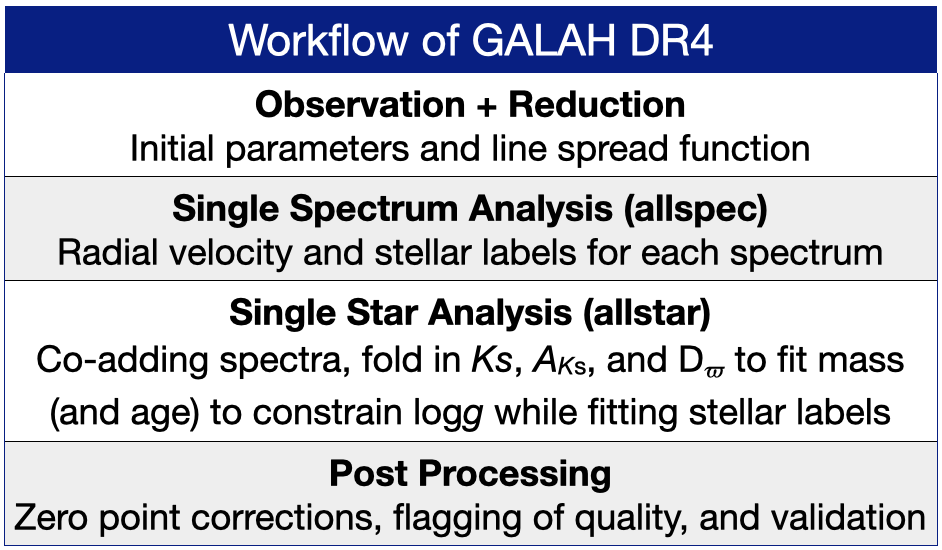
\includegraphics[width=\textwidth]{figures/workflow_galah_dr4.png}
 \caption{\textbf{Workflow of GALAH DR4}}
 \label{fig:workflow_galah_dr4}
\end{figure}

%%%%%%%%%%%%%%%%%%%%%%%%%%%%%%%%%%%%%%%%%%%%%%%%%%%%%%%%%%%%%%%%%%%%%%%%%
\section{DATA}
\label{sec:data}
%%%%%%%%%%%%%%%%%%%%%%%%%%%%%%%%%%%%%%%%%%%%%%%%%%%%%%%%%%%%%%%%%%%%%%%%%

The GALAH Survey uses the 3.9-metre Anglo-Australian Telescope at Siding Spring Observatory on Gamilaraay Country and its Two-Degree Field positioning system (2dF) top end \citep{Lewis2002}. 2dF magnetically places up to 400 fibre entrances on one of two metal field plates, which can be tumbled to allow observing of one set of fibres while configuring the other. Light is delivered through the fibres to the High Efficiency and Resolution Multi-Element Spectrograph (HERMES) spectrograph \citep{Barden2010, Brzeski2011, Heijmans2012, Farrell2014, Sheinis2015} and dispersed into four non-contiguous wavelength bands in the optical. The data used in this data release is primarily based on observations of stars with said setup, but also makes us of auxiliary photometric and astrometric information for the stars where available.

In this Section, we describe which stars we have targeted and observed (Sec.~\ref{sec:target_selection_observations}) with the 2dF-HERMES setup, including the first description of the second phase of GALAH observations (GALAH Phase 2) with a sharper focus on main-sequence turnoff stars to estimate more precise ages. In Sec.~\ref{sec:spectroscopic_data_from_galah_observations}, we briefly summarise the properties of the spectroscopic data and how they were reduced to one-dimensional spectra. We also point out major changes in the observations and reductions with respect to the previous (third) data release \citep{Buder2021}. We further elaborate on the auxiliary information that was used for the analysis in Sec.~\ref{sec:non-spec_data}.

%%%%%%%%%%%%%%%%%%%%%%%%%%%%%%%%%%%%%%%%%%%%%%%%%%%%%%%%%%%%%%%%%%%%%%%%%
\subsection{Target selection and observational setup} \label{sec:target_selection_observations}
%%%%%%%%%%%%%%%%%%%%%%%%%%%%%%%%%%%%%%%%%%%%%%%%%%%%%%%%%%%%%%%%%%%%%%%%%

GALAH DR4 is a combination of the main GALAH survey and additional projects to observe asteroseismic targets from the K2 \cite{Sharma2019} and TESS missions \cite{Sharma2018}, as well as hand-picked and random observations of globular and open cluster members. The column \texttt{survey\_name} in our catalogues denotes this origin.

\subsubsection{Target selection for GALAH Phase 1 and 2}

For GALAH Phase 1, we used the 2MASS photometric survey \citep{Skrutskie2006} with its $J$ and $Ks$ filters as a parent sample from which we selected stars within estimated visual magnitudes
\begin{equation}
V_\mathrm{JK} = K_S+2(J-K_S+0.14)+0.382e^{((J-K_S-0.2)/0.5)}.
\end{equation}

For GALAH Phase 1, a tiling pattern (with unique \texttt{field\_id} entries) with $2\,\mathrm{deg}$ fields of view below declination $\delta < +10\,\mathrm{deg}$ were created for regions with Galactic latitude $\vert b \vert > 10\,\mathrm{deg}$ to avoid crowding and strong extinction. For each tile, a selection of 400 stars within magnitudes $9 < V_\mathrm{JK} < 12$ for a bright magnitude cut and $12 < V_\mathrm{JK} < 14$ for the nominal magnitude cut is randomly selected from the complete parent sample of 2MASS. This typically selects 2/3 main sequence and turnoff stars and 1/3 evolved stars.

For GALAH Phase 2, a stronger focus on turn-off stars was implemented with the photometric and astrometric information of \Gaia data release 2 as parent sample. For each field, we therefore first allocate fibres to stars with absolute magnitude between $2 < M_G < 4$, where
\begin{equation}
M_G = \texttt{phot\_g\_mean\_mag} + 5 \cdot \log_{10} \left( \frac{\texttt{parallax}}{100\,\mathrm{mas}} \right)
\end{equation}
with $G$ magnitude and parallax measurements from \Gaia DR2 \citep{Brown2018, Evans2018, Lindegren2018}. Remaining fibres are again filled with targets as done in Phase 1.

\subsubsection{Observational setup}

\begin{table}
\centering
 \caption{\textbf{Overview of stars observed for the programs included in this data release.} Numbers of open and globular cluster observations were estimated after observations as described in Sec.~\ref{sec:oc_gc}. We have observed 18 globular clusters (13 with $\geq$ 5 stars) and 286 open clusters (94 with $\geq$ 5 stars).}
\label{tab:field_ids}
\begin{tabular}{crcr}
\hline \hline
Program & No. Stars & Program & No. Stars \\
\hline
galah\_bright & 65\,188 & 
k2\_hermes & 117\,708\\
galah\_main & 427\,699 & 
tess\_hermes & 37\,228\\
galah\_faint & 25\,802 & 
globular clusters & 1\,185\\
galah\_phase2 & 125\,058 & 
open clusters & 4\,487\\
commissioning & 2\,625 & 
other & 20\,308\\
  \hline
 \end{tabular}
\end{table}

\begin{figure*}[ht]
 \centering
 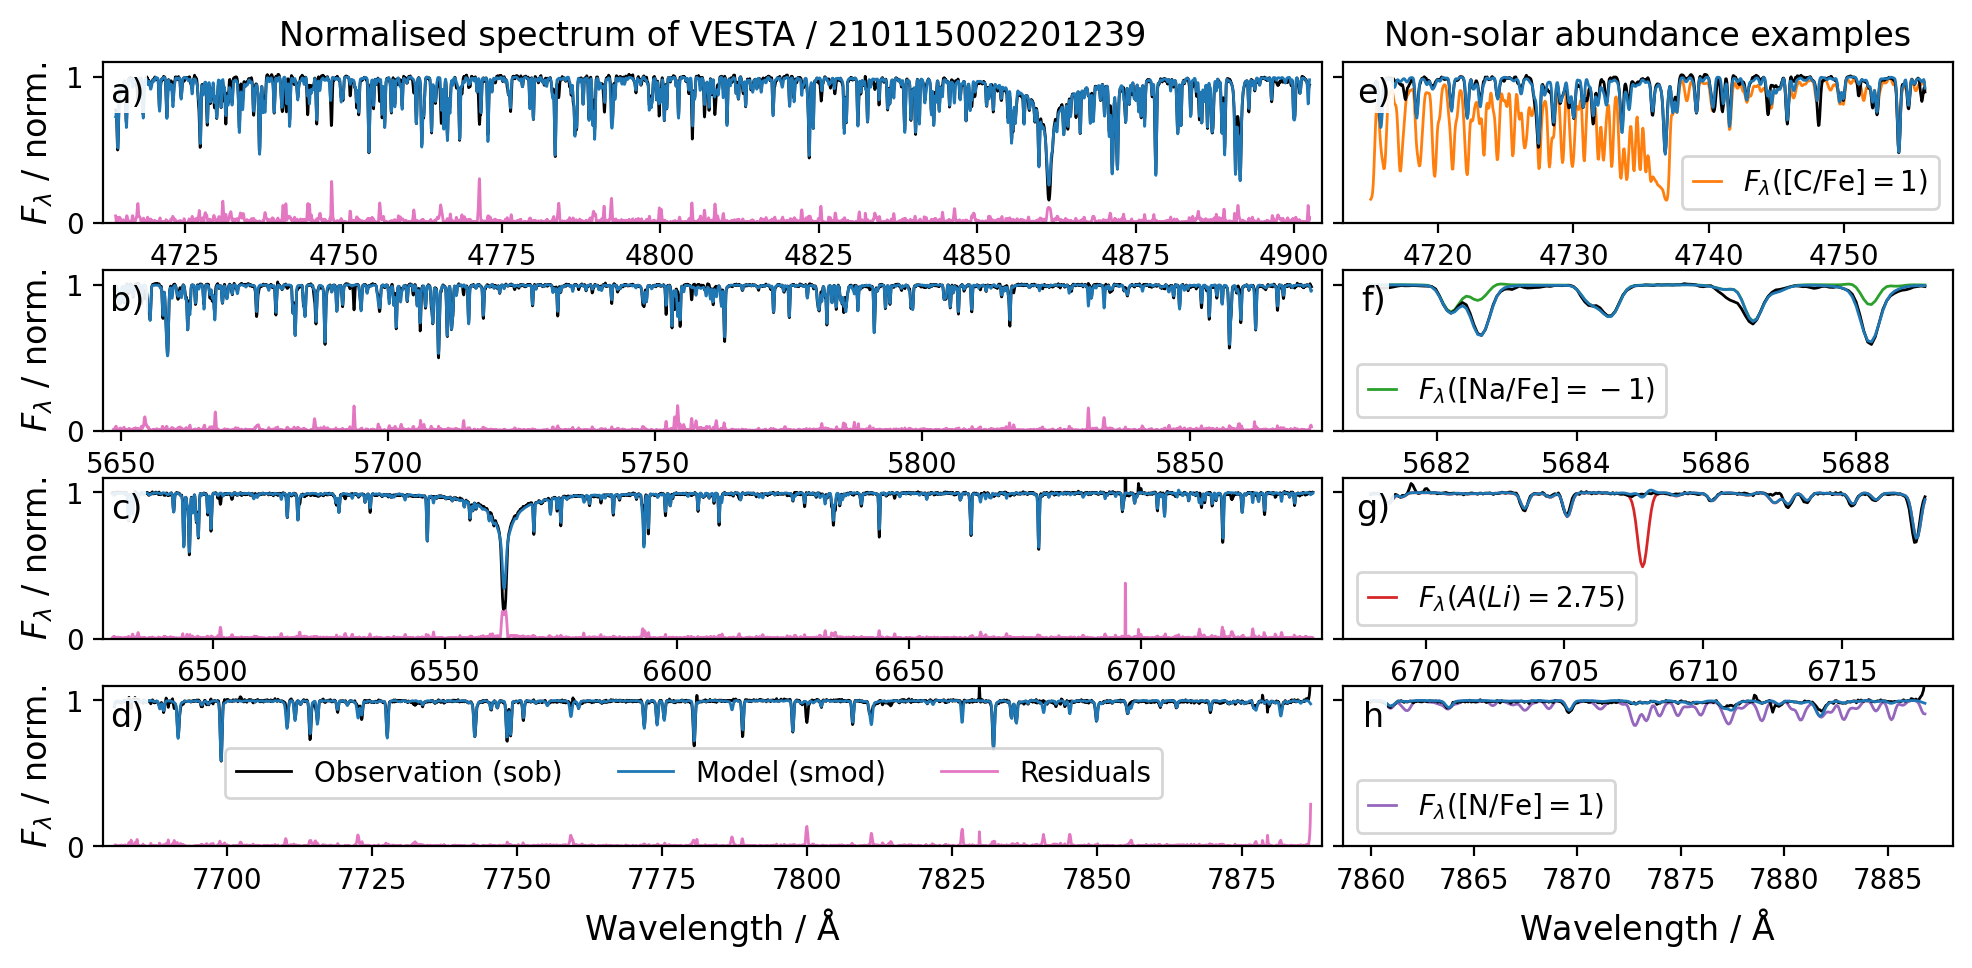
\includegraphics[width=\textwidth]{figures/210115002201239_abundance_examples.png}
 \caption{\textbf{Comparison of normalised observed (black) and synthetic spectra (blue) of the asteroid 4 Vesta with solar composition as well as examples of synthetic spectra with non-solar abundances.}
 \textbf{Panels a-d)} show the observed and best-fit synthetic spectrum as well as their absolute residual (pink) for the four wavelength channels of the HERMES spectrograph.
 \textbf{Panel e)} shows the beginning of the blue CCD 1 (left-most part of panel a) with an additional synthetic spectrum with ten times higher [C/Fe] in orange, for which the $\mathrm{C}_2$  Swan bands are prominent.
 \textbf{Panel f)} shows the beginning of the green CCD 2 (left-most part of panel b) and exemplifies with a synthetic spectrum in green that also a ten times lower [Na/Fe] abundance (for example, in accreted stars) can still be reliably detected. 
 \textbf{Panel g)} shows the end of the red CCD 3 with a synthetic spectrum of primordial Li abundance of $\mathrm{A(Li)} = 2.75$ in red. While this abundance could be detected, the the line for the Solar value $\mathrm{A(Li)} = 1.05$ is barely detectable.
 \textbf{Panel h)} shows the end of the infrared CCD 4, which would show strong molecular absorption features of the CN molecule for $\mathrm{[N/Fe]} = +1$ (purple).
 }
 \label{fig:210115002201239_abundance_examples}
\end{figure*}

We list the observations under various sub-programs in Table~\ref{tab:field_ids}. Except for 2\,935 spectroscopic observations with the high-resolution mode of HERMES ($R \sim 42\,000$) on 7, 8, 10, 11 and 12 February 2014, all observations were made in the low-resolution mode ($R \sim 28\,000$). Exposure times depend on the program. Under sufficient conditions (no clouds and seeing below $2\,\mathrm{arcsec}$), GALAH Phase 1 and TESS-HERMES observed 3x6 minutes for bright targets ($9 < V_\mathrm{JK} < 12$) and 3x20 minutes for the majority of targets ($12 < V_\mathrm{JK} < 14$). GALAH Phase 2 extended these times to 3x10 and 3x30 minutes, respectively, and included repeat observations of GALAH Phase 1 main targets with another 3x15 minutes. K2-HERMES observations targeted stars with $13 < V_\mathrm{JK} < 15$ or even $13 < V_\mathrm{JK} < 15.8$ to complement the K2 Galactic Archaeology Program \citep{Stello2015}. These fields were observed for 2 hours, similar to most globular and open cluster stars. Worse seeing conditions or thin clouds triggered between one ($2 < \mathrm{seeing} < 2.5\,\mathrm{arcsec}$) and 3 ($2.5 < \mathrm{seeing} < 3\,\mathrm{arcsec}$) additional exposures. In addition to the science frames, quartz fibre flat and ThXe arc lamp observations were taken directly before or after each set of science exposures, and bias frames were taken at the beginning or end of each observing night.

%%%%%%%%%%%%%%%%%%%%%%%%%%%%%%%%%%%%%%%%%%%%%%%%%%%%%%%%%%%%%%%%%%%%%%%%%
\subsection{Spectroscopic data from GALAH observations}
\label{sec:spectroscopic_data_from_galah_observations}
%%%%%%%%%%%%%%%%%%%%%%%%%%%%%%%%%%%%%%%%%%%%%%%%%%%%%%%%%%%%%%%%%%%%%%%%%

Since the commissioning of the HERMES spectrograph in late 2013 until 6 August 2023, the GALAH collaboration and its partners have observed and successfully reduced \allspecnumber spectra of \allstarnumber stars. The spectroscopic data are collected by four separate CCDs that cover $\sim 1000\,\text{\AA}$ in the range of $4713-4903$ (blue CCD or CCD1), $5648-5873$ (green / CCD2), $6478-6737$ (red / CCD3), and $7585-7887\,\text{\AA}$ (infrared IR / CCD4), as can be seen from the reduced example spectrum of the asteroid 4 Vesta in Fig.~\ref{fig:210115002201239_abundance_examples}. The reduction process to create FITS files of reduced spectra from two-dimensional images of the cameras employs an updated and publicly available \href{https://github.com/sheliak/galah_reduction/blob/master/extract6.0.py}{version 6} of the already well-tested reduction pipeline \citep{Kos2017}. The extensions of these files are listed in Tab.~\ref{tab:reduction_fits} and created as follows.

\begin{table}
    \centering
    \caption{Data product 1: FITS files of reduced spectra}
    \label{tab:reduction_fits}
    \begin{tabular}{cc}
    \hline \hline
    FITS Ext. & Description \\
    \hline
    Ext. 0 & Un-normalised signal~/~counts \\
    Ext. 1 & Normalised signal (by reduction pipeline) \\
    Ext. 2 & Relative uncertainty of signal \\
    Ext. 3 & Subtracted sky signal~/~counts \\
    Ext. 4 & Applied telluric correction \\
    Ext. 5 & Scattered light~/~counts \\
    Ext. 6 & Cross-talk \\
    Ext. 7 & Resolution profile~/~FWHM \\
    \hline
    \end{tabular}
\end{table}

Science frames are corrected by removing the bias, dividing out the different gain of the two readout amplifiers per CCD, flagging bad pixels, and dividing by master flatfield frames, as well as removing cosmic rays and scattered light. Subsequently, apertures for each fibre trace are identified and used to extract the individual spectra. 

Wavelength calibrations are performed via Chebyshev polynomial functions based on the ThXe arc frames and the spectra are interpolated onto a linearly increasing wavelength grid. The starting wavelength \texttt{CRVAL1} and dispersion \texttt{CDELT1} are saved in the headers of each FITS file.

Finally, sky lines are subtracted and telluric features removed, before a barycentric correction is applied to create the 'reduced' spectra that are saved in extension~1 of the reduction pipeline FITS files and used for the subsequent analysis. 

Fractional noise / uncertainties are saved in extension~2 and calculated from the square root of the sum of flux, sky features (extension~3), scattered light (extension~5), crosstalk (extension~6) and the squared readout noise.

The wavelength dependent line spread functions (LSFs) are measured from the arc calibration frames for each spectrum and CCD by fitting modified Gaussian distributions with a boxiness parameter $b$ and full width half maximum \texttt{fwhm} for each wavelength point in the spectrum, that is
\begin{align}
    \exp \left(-0.693147 \cdot \vert 2 \cdot \textbf{\textit{x}}/\texttt{fwhm} \vert^\texttt{b}\right) \label{eq:lsf}
\end{align}
The array $\textbf{\textit{x}}$ then includes the pixels around each wavelength step that are used to apply the convolution from higher resolution to GALAH resolution spectra. The fitted values of $fwhm$ are saved in extension~7 with $b$ saved in the headers.

\SB{Should we elaborate on any overall information, like SNR overview and pointing on the sky?}
\SB{Elaborate on how the reduction pipeline parameters \texttt{teff\_r} etc. are estimated.}

%%%%%%%%%%%%%%%%%%%%%%%%%%%%%%%%%%%%%%%%%%%%%%%%%%%%%%%%%%%%%%%%%%%%%%%%%
\subsection{Auxiliary data from \Gaia, 2MASS, and literature} \label{sec:non-spec_data}
%%%%%%%%%%%%%%%%%%%%%%%%%%%%%%%%%%%%%%%%%%%%%%%%%%%%%%%%%%%%%%%%%%%%%%%%%

%SELECT
%galah.sobject_id,
%tmass.designation as tmass_id,
%tmass.ph_qual as tmass_ph_qual,
%tmass.ra as raj2000,
%tmass.dec as dej2000,
%tmass.j_m, tmass.j_msigcom,
%tmass.h_m, tmass.h_msigcom,
%tmass.ks_m, tmass.ks_msigcom,
%calj.r_med_geo,calj.r_lo_geo,calj.r_hi_geo,
%calj.r_med_photogeo,calj.r_lo_photogeo,calj.r_hi_photogeo,
%calj.flag as calj_flag,
%gaia.*
%FROM gaiadr3.gaia_source as gaia
%LEFT OUTER JOIN
%	external.gaiaedr3_distance as calj
%	ON calj.source_id = gaia.source_id
%LEFT OUTER JOIN
%	gaiadr3.tmass_psc_xsc_best_neighbour AS tmassxmatch
%	ON tmassxmatch.source_id = gaia.source_id
%LEFT OUTER JOIN
%	gaiadr3.tmass_psc_xsc_join AS tmass_join
%	ON tmass_join.clean_tmass_psc_xsc_oid = tmassxmatch.clean_tmass_psc_xsc_oid
%LEFT OUTER JOIN
%	gaiadr1.tmass_original_valid as tmass
%	ON tmass.designation = tmass_join.original_psc_source_id
%INNER JOIN
%	user_sbuder.dr6_0_230101_unique_ids as galah
%	ON galah.tmass_id = tmass.designation

To support our spectroscopic analysis, we make use of astrometric and photometric information from the \Gaia satellite \citep{Gaia-Collaboration2016} and 2MASS survey \citep{Skrutskie2006}, which is available for essentially all our targets. We further use the value-added catalogues, like distance estimates for field stars by \citep{BailerJones2021} as well as open and globular cluster membership probabilities from \citet{CantatGaudin2020} as well as \citet{Vasiliev2021} and \citet{Baumgardt2021}.

\subsubsection{\Gaia DR3}

We crossmatch our observations to the \Gaia DR3 catalogue \citep{Brown2021,GaiaDR3} using the 2MASS ID, via the nearest neighbour crossmatches provided as part of \Gaia DR3 \citep{Torra2021}. 
911\,754 (99.0\,\%) also have astrometric information \citep{Lindegren2021a} and 849\,867 (93.0\,\%) have radial velocity estimates \citep{Katz2022}. We apply the corrections to both photometric \citep{Riello2021} and astrometric \citep{Lindegren2021b}information. Where possible we prefer the photogeometric distances over the geometric distances from \citep{BailerJones2021}. Where neither are available, we further try to find parallaxes from \cite{vanLeeuwen2007}. The average parallax uncertainty of the GALAH stars is $\sigma_{\varpi} / \varpi = 1.6_{-0.9}^{+2.6}\,\mathrm{\%}$. Only $2.3\,\%$ of GALAH stars have no parallax measurements or parallax measurements beyond $20\%$ uncertainty, for which the priors adopted by \citep{BailerJones2021} start to dominate distance estimates.

\subsubsection{2MASS, WISE, and extinction}

In addition to the excellent infrared photometry for 99.9\,\% of our sources from the 2MASS survey \citep{Skrutskie2006}, 98.7\,\% of them have far-infrared measurements from the WISE mission \citep{Cutri2013}. We therefore can estimate the extinction in the $K_S$ band via the RJCE method \citep{Majewski2011} $A_{K_S}  = 0.917 \cdot \left( H - W2 - 0.08 \right)$ for most stars. We confirm this estimate by estimating the extinction in $K_S$ via the extrapolation of the color extinction of $B-V$, that is, $A_{K_S} \sim 0.36 \cdot E(B-V)$ \citep{Cardelli1989}. We revert to this value if it is less than half the value of the RJCE estimate, or if either of the H and W2 bands does not have an excellent quality flag 'A'. For negative estimates by the RJCE method and very nearby stars ($<100\,\mathrm{pc}$) we null the value.

\subsubsection{Open and Globular Cluster members and distances} \label{sec:oc_gc}

We identify open cluster members using the membership catalogue from \citet{CantatGaudin2020} via crossmatch with the \Gaia \texttt{source\_id} and adjust their parallaxes and distance estimates to the average cluster values if the latter are more precise. We identify globular cluster members (with more than 70\% probability) via the membership catalogue from \citet{Vasiliev2021} by crossmatching with the \Gaia \texttt{source\_id}. We then adjust the parallaxes and distances for the member stars to the mean values listed by \citet{Baumgardt2021}.

%%%%%%%%%%%%%%%%%%%%%%%%%%%%%%%%%%%%%%%%%%%%%%%%%%%%%%%%%%%%%%%%%%%%%%%%%
\section{SYNTHETIC SPECTRA FOR 2DF-HERMES}
\label{sec:synthetic_spectra}
%%%%%%%%%%%%%%%%%%%%%%%%%%%%%%%%%%%%%%%%%%%%%%%%%%%%%%%%%%%%%%%%%%%%%%%%%

The aim of our spectroscopic analysis is to estimate the best set of stellar properties (labels) that influence a stellar spectrum by minimising the difference between observed stellar spectra and synthetic ones that were created with those best stellar labels. In our endeavour to push the limits even further, we are advancing our analysis to fit all 31 elemental abundances and stellar parameters across the full GALAH wavelength range simultaneously with the appropriate model spectrum.

To make this computationally feasible, we follow an idea reported by \citet{Rix2016} and create flexible models for smaller regions of the parameter space from only a limited number of \textit{ab initio} models \citep[see also][]{Ting2016b}. Our \textit{ab initio} models are calculated with Spectroscopy Made Easy \citep[\textsc{sme}][]{Valenti1996,Piskunov2017} for the whole wavelength range and all visible atomic and molecular lines for random selections of elemental abundances and stellar parameters within the range of \marcs atmospheres \citep{Gustafsson2008} at much higher resolution and sampling than our HERMES spectra. We then select subsets of these spectra within a restricted space of the three main spectroscopic parameters \Teff, \logg, and \feh. This idea is comparable to selecting Solar or stellar twin spectra when analysing the Sun \citep[see e.g.]{Nissen2015} or differential abundance analysis of globular cluster stars \citep[e.g.]{Yong2013, Monty2023}. As they cancel out several systematic issues of line data and atmospheric effect, these approaches have been highly successful \citep{Nissen2018}. For each subset, we train a neutral network that correlates stellar flux and labels (stellar parameters and abundances) similar to \textit{The Payne} \citep{Ting2019}. With these models, we can then create model spectra with all lines over the whole wavelength range for any combination of element abundances within this restricted parameter space within less than a second (as compared to minutes or hours for physics-driven syntheses). 

Another reason to create smaller training sets rather than a "one-fit-all" approach was the limited flexibility of both quadratic and non-linear interpolation routines within computationally reasonable model sizes and ability to test the model accuracy over the full parameter space. Surveys like GALAH, RAVE and APOGEE aim to fit basically all types of spectra at once. This means we demand one model to predict Sun-like stars, red clump stars, metal-poor stars with almost no absorption features, cool evolved stars with strong molecular features, and hot stars with shallow and broad lines - all at once and for up to 31 elemental abundances. As one can imagine, this is an impossible task and has led to numerous systematic trends in catalogues for the most extreme cases that use such model interpolations \citet{Casey2016,Buder2018,Ting2019}. In this data release, we therefore purposefully limit the spectral complexity by creating smaller models. The hot star model therefore does not need to also predict the strong molecular absorption features of a cool star. We discuss the possible caveats and disadvantages of this approach and our particular implementation in Sec.~\ref{sec:caveats}.

In this section, we lay out how we create smaller bins in the parameter space from which we sample a training set (Sec.~\ref{sec:higher_resolution_synthetic_spectra}) rather than using one training set for all stars. We lay out how we create the parent sample of high-resolution synthetic stellar spectra (Sec.~\ref{sec:higher_resolution_synthetic_spectra}) and train neural networks to quickly predict/interpolate new synthetic spectra (Sec.~\ref{sec:interpolating_synthetic_spectra_with_neural_networks}).

%%%%%%%%%%%%%%%%%%%%%%%%%%%%%%%%%%%%%%%%%%%%%%%%%%%%%%%%%%%%%%%%%%%%%%%%%
\subsection{Stellar twin training sets rather than one-fits-all}
\label{sec:spectrum_grid}
%%%%%%%%%%%%%%%%%%%%%%%%%%%%%%%%%%%%%%%%%%%%%%%%%%%%%%%%%%%%%%%%%%%%%%%%%

\begin{figure}[ht]
 \centering
 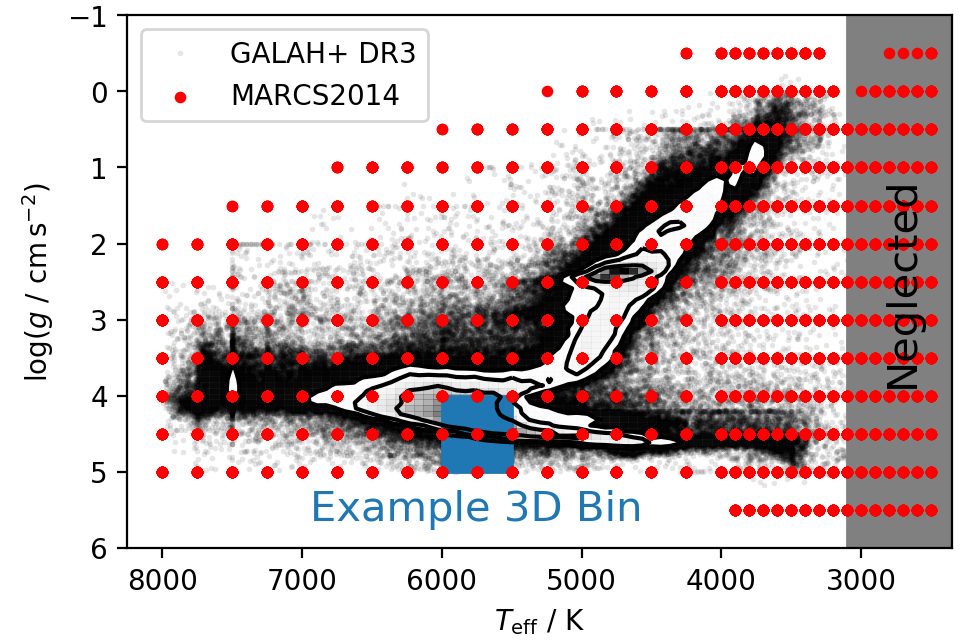
\includegraphics[width=\textwidth]{figures/teff_logg_grid_coverage.png}
 \caption{\textbf{Coverage in \Teff and \logg of the MARCS2014 grid (red) and GALAH DR3 (black, including density countours).} Shown is also an example of one of the 3D bins used to create models with \TheCannon. MARCS grid points \Teff$ < 3100\K$ or \feh$<-3\dex$ are neglected throughout GALAH DR4.}
 \label{fig:teff_logg_grid_coverage}
\end{figure}

The base grid for our training set computation is the \marcs grid \citep{Gustafsson2008}, which is shown with red points in Fig.~\ref{fig:teff_logg_grid_coverage}. Following the aforementioned idea of restricting ourselves to stellar siblings, we create multiple 3-dimensional bins in \Teff, \logg, and \feh within $\pm 1$ grid points in \Teff (with either $\pm 250$ or $\pm 100\K$), \logg ($\pm 0.5\dex$), and \feh ($\pm 0.5$ or $\pm 0.25\dex $). An example box is shown for Solar siblings as a blue box in Fig.~\ref{fig:teff_logg_grid_coverage}, which is centred on $T_\text{eff} = 5750\pm250\K$, $\log g = 4.5\pm0.5\dex$ and $\mathrm{[Fe/H]} = 0.0\pm0.25\dex$.

Within these bins we sample 280\footnote{This number is chosen to match the 28 CPUs of our computing nodes.} synthetic spectra with no rotational broadening, which are later broadened with different rotational velocities \vsini to create between 1680 and 2240 training set spectra for each bin. 
%We explain the sampling of parameters and abundances in an exemplary way for the 3D bin centred on $T_\text{eff} = 5750\pm250\K$, $\log g = 4.5\pm0.5\dex$ and $\mathrm{[Fe/H]} = 0.0\pm0.25\dex$ (see blue box in Fig.~\ref{fig:teff_logg_grid_coverage}).

\begin{figure*}[ht]
 \centering
 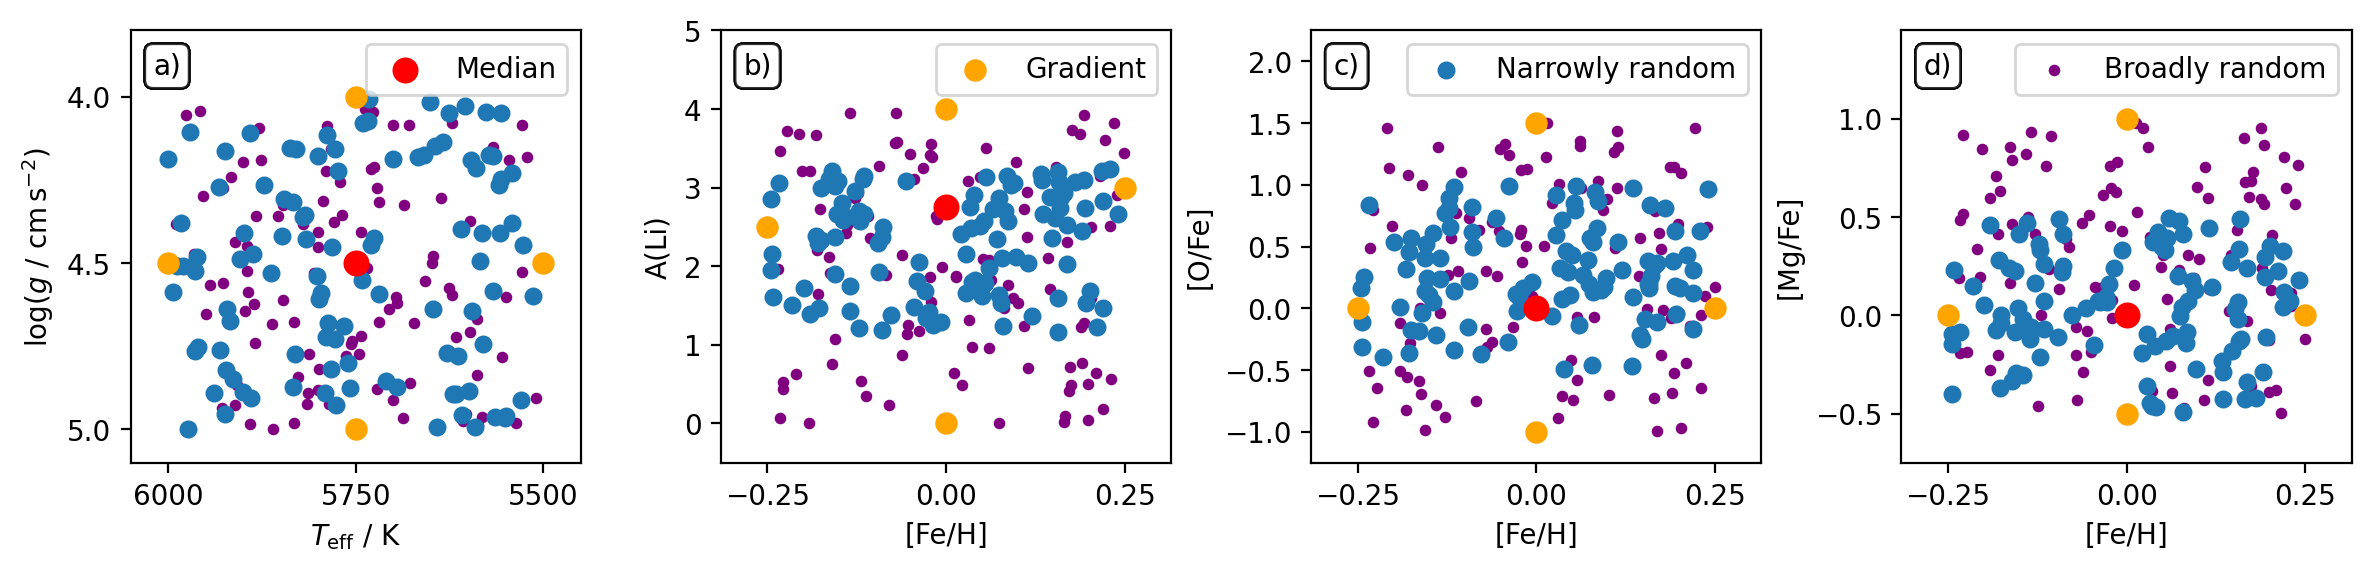
\includegraphics[width=\textwidth]{figures/example_3d_bin_sample.png}
 \caption{\textbf{Coverage of stellar parameters and abundances for one of the 3D bins.} Shown is the example of the Solar 3D bin ($T_\mathrm{eff}~/~\mathrm{K} = 5750$, $\log g~/~\mathrm{dex} = 4.5$, $\mathrm{[Fe/H]}~/~\mathrm{dex} = 0.0$). \textbf{Panel a):} \Teff and \logg, \textbf{Panel b):} [Fe/H] vs. A(Li), \textbf{Panel c):} [Fe/H] vs. [O/Fe], \textbf{Panel d):} [Fe/H] vs. [Mg/Fe]. While \Teff, \logg, and \feh are sampled randomly within the 3D bin, the abundances are sampled both narrowly (blue) and broadly (purple) within limits as described in the text. Red points indicate the median label values and orange points the adjusted label values to test the gradient change of spectra with individual labels.}
 \label{fig:example_3d_bin_sample}
\end{figure*}


\begin{table*}[ht]
\centering
 \caption{Example of boundaries for the uniform sampling of synthetic spectrum labels (stellar parameters and elemental abundances) for the 3-dimensional bin of Solar siblings \texttt{5750\_4.50\_0.00}.}
\label{tab:sampling_xfe}
\begin{tabular}{lclclc}
\hline \hline
Parameter & Sampling & Element & Sampling Narrow & Element & Sampling Broad \\
\hline
$T_\text{eff}~/~\K$ & 5500..5750..6000 & $\mathrm{A(Li)}$ & {1.05..2.75..3.26} & $\mathrm{A(Li)}$ & {0.00..4.00} \\
$\log g~/~\dex$ & 4.0..4.5..5.0 &  $\mathrm{C,~N,~O}$ & {-0.5..0.0..1.0} & $\mathrm{C,~N,~O}$ & {-1.0..1.5} \\
$\mathrm{[Fe/H]}~/~\dex$ & {-0.25..0.0..0.25} & $\mathrm{Y,~Ba,~La,~Ce,~Nd}$ & {-0.5..0.0..1.0} & $\mathrm{Y,~Ba,~La,~Ce,~Nd}$ & {-1.0..1.5} \\
$v_\text{mic}~/~\kms$ & {0.5,1.5,4.0}, but see Eq.~\ref{eq:vmic_initial} & $\mathrm{[X/Fe]~for~Mg,~Si,~Ti}$  &  {-0.5..0.0..0.5}& $\mathrm{[X/Fe]~for~Mg,~Si,~Ti}$ & {-0.5..1.0} \\
$v \sin i~/~\kms$ & 0.0\text{, but see Eq.~\ref{eq:vsini}} & $\mathrm{[X/Fe]~for~all~other~elements}$ & {-0.5..0.0..0.5} & $\mathrm{[X/Fe]~for~all~other~elements}$ & {-1.0..1.0}  \\
\hline \hline
\end{tabular}
\end{table*}

Stellar parameters (\Teff, \logg, \feh, \vmic) and elemental abundances [X/Fe] of all 30 elements are randomly sampled within reasonable limits (see examples in Tab.~\ref{tab:sampling_xfe}) and fed into \sme to create self-consistent synthetic spectra over the full HERMES wavelength range for \marcs atmospheres. 

\vmic values are sampled uniformly between the upper and lower limits of the empirical relation from GALAH DR3 \citep[Eqs.~4 and 5 from][]{Buder2021} and an adjusted version of the relation by \citet{DutraFerreira2016}. The latter has been adjusted for $T_\text{eff}^\prime = T_\text{eff} - 5500\,\mathrm{K}$ as well as $\log g^\prime = \log g - 4.0$ to return:
\begin{align} 
v_\text{mic} = \begin{array}{l}
1.198 + 3.16 \cdot 10^{-4} \cdot T_\text{eff}^\prime - 0.253 \cdot \log g^\prime \\ - 2.86\cdot 10^{-4} \cdot T_\text{eff}^\prime \cdot \log g^\prime + 0.165 \cdot (\log g^\prime)^2
\end{array} \label{eq:vmic_initial}
\end{align}

%%%%%%%%%%%%%%%%%%%%%%%%%%%%%%%%%%%%%%%%%%%%%%%%%%%%%%%%%%%%%%%%%%%%%%%%%
\subsection{Higher-resolution synthetic spectra with \sme}
\label{sec:higher_resolution_synthetic_spectra}
%%%%%%%%%%%%%%%%%%%%%%%%%%%%%%%%%%%%%%%%%%%%%%%%%%%%%%%%%%%%%%%%%%%%%%%%%

We create training sets from high-resolution stellar spectra for each smaller 3D bin region of the parameter space. We compute over-sampled synthetic intensity spectra at ten times higher resolution then the typical GALAH resolution with \sme for seven equal-area angles of a stellar surface (see Fig.~\ref{fig:sme_mu_output}).

\begin{figure}[hbt]
 \centering
 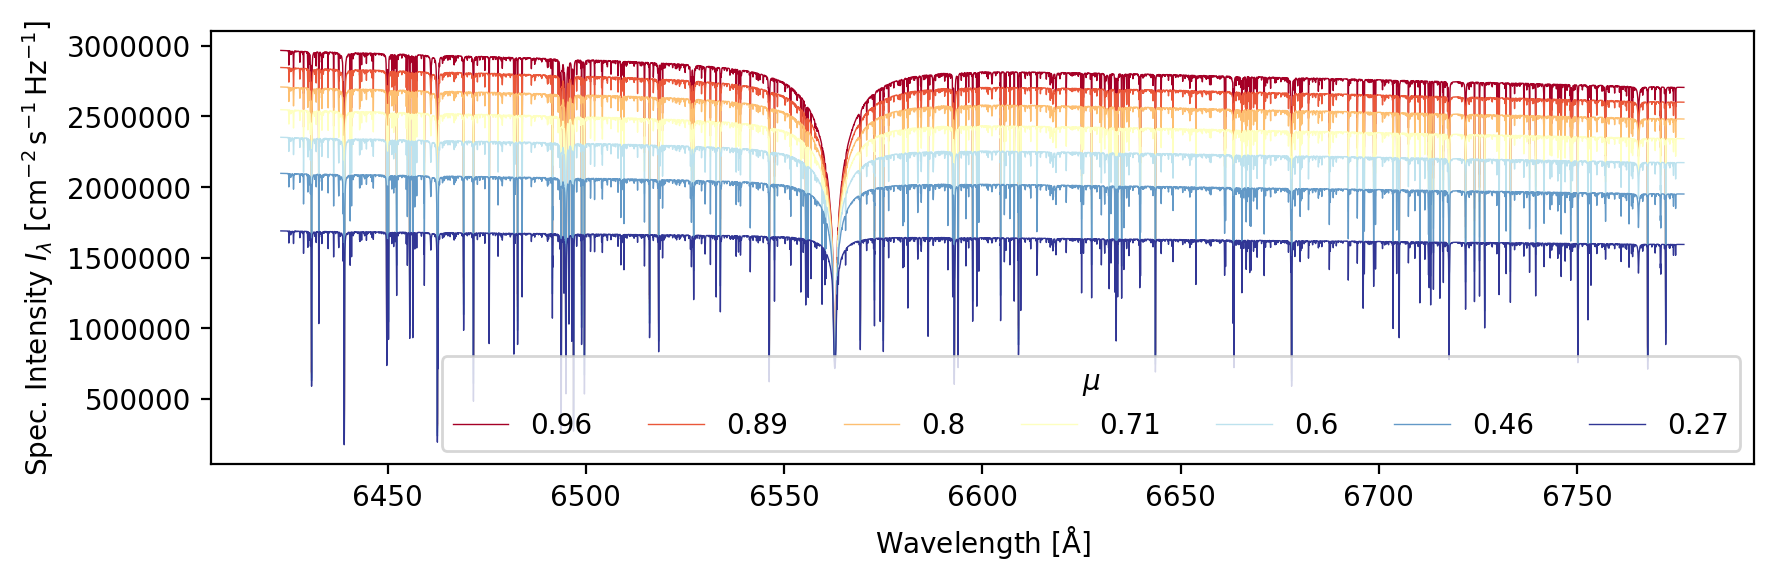
\includegraphics[width=\textwidth]{figures/solar_twin_specific_intensity.png}
 \caption{\textbf{Example output of \sme for a solar spectrum in HERMES CCD3 (around the Balmer $\mathrm{H}_\alpha$ line).} Shown are the the specific intensities (\texttt{sme.sint}) as a function of the equal-area midpoints of each equal-area annulus $\mu$.}
 \label{fig:sme_mu_output}
\end{figure}

For each spectrum, we first run a test on all available lines in the GALAH linelist, which is adapted from \citet{Heiter2021} and includes small changes to correct wrong $\log gf$ values for a few lines within the GALAH wavelength range. We keep all atomic lines for the final synthesis and restrict the molecular lines to those with \textsc{sme}.depth above 0.001.

Spectra are computed at a resolution of $R = 300,000$ on a fine wavelength grid with 60,819 pixels spread over the extended wavelengths $4675.1-4949.9$, $5624.1-5900.9$, $6424.1-6775.9$, and $7549.1-7925.9 \Angstroem$. We note that these extend significantly beyond the actual GALAH wavelength range.

We use 1D \marcs atmospheres from the \marcs grid \citep[][version 2014]{Gustafsson2008} and interpolate them for combinations of \Teff, \logg, and \feh. We use grids of non-LTE departure coefficients by \citet{Amarsi2020} for H, Li, C, N, O, Na, Mg, Al, Si, K, Ca, Mn, and Ba. For all except C, we use grids that include background scattering.

Our synthetic grid explicitly includes C and N abundances. C was previously included in the analysis of GALAH DR3, but limited to the atomic C line. The analysis thus neglected the molecular absorption features of $\mathrm{C_2}$ and CN at the beginning of CCD1 and end of CCD4, respectively. With the new self-consistent grid, we can include these features, as they hold valuable information for both C and N, as well as several other features through the molecular equilibrium in stars \citep[see e.g.][]{Ting2018}.

To be able to test that the flux-label correlations found by our polynomial interpolation are limited to reasonable wavelength ranges, we also calculate one spectrum that is exactly in the middle of the parameter range and additional spectra, where we increase the value of one label at a time (e.g. increase [O/Fe] by $1\dex$) to test the response in the synthetic spectrum.

To save computational costs, we compute synthetic spectra with no rotational or macroturbulence broadening ($v_\text{mac} = v\sin i = 0\kms$), but save the model continuum flux (\texttt{sme.cmod}) and the specific intensities (\texttt{sme.sint}) as a function of the equal-area midpoints of each equal-area annulus $\mu$ (see Fig.~\ref{fig:sme_mu_output}). We then apply the broadening of spectra due to rotation (\vsini) with the flux integration code of the python-implementation \textsc{PySME} \citep{Wehrhahn2021} of \textsc{SME} \citep{Piskunov2017}. Depending on the expected rotational velocities (increasing with temperature) we sample a range of
\begin{align} \label{eq:vsini}
    v \sin i~/~\kms \in \{ 1.5, 3, 6, 9, 12, 18, 24, 36\}.
\end{align}

Note that $v \sin i = 24 \kms$ is only included for bins with \Teff$\geq 5000\,\mathrm{K}$ and $v \sin i = 36 \kms$ for those with \Teff$\geq 6000\,\mathrm{K}$.

% The decision for these values was made based on the distribution of \vsini ($7.2_{-1.6}^{4.9}\kms$ with 90\% between 4.7 and $29.0\kms$) in GALAH+ DR3 \citep{Buder2021} and comparison with the grid values used by APOGEE DR16 \citep{Joensson2020}.

%%%%%%%%%%%%%%%%%%%%%%%%%%%%%%%%%%%%%%%%%%%%%%%%%%%%%%%%%%%%%%%%%%%%%%%%
\subsection{Interpolating synthetic spectra with neural networks} \label{sec:interpolating_synthetic_spectra_with_neural_networks}
%%%%%%%%%%%%%%%%%%%%%%%%%%%%%%%%%%%%%%%%%%%%%%%%%%%%%%%%%%%%%%%%%%%%%%%%

To allow a fast interpolation with new and different stellar labels, we use the method of training descriptive models to connect stellar fluxes at given pixels from a combination of stellar labels. This method is well established in stellar spectroscopy through the successful applications of quadratic models with \textit{The Cannon} \citep[see e.g.][]{Ness2015, Ness2016, Casey2016, Casey2017, Ho2017, Buder2018} as well as neural networks with \textit{The Payne} \citep[see e.g.][]{Ting2019, Xiang2019, Xiang2021}. Because of the needed flexibility\footnote{For a more detailed discussion on the advantages of neural networks for predicting spectra see \citet{Ting2019}.} to predict synthetic spectra with 36 stellar labels for a large parameter space, we are also choosing neural networks to interpolate between our synthetic spectra in this data release.

In particular, we use the neural network architecture and training algorithms similar to \textit{The Payne} \citep{Ting2019} for our data. We describe the connection of stellar labels $\boldsymbol{\ell}$ and the flux $f$ at each wavelength pixel $\lambda$ via
\begin{equation}
f_\lambda = w \cdot \mathrm{lReLU} \bigg( \tilde{w}_\lambda^i \cdot \mathrm{lReLU}  \Big( w^k_{\lambda i} \ell_k + b_{\lambda i} \Big) + \tilde{b} \bigg) + \bar{f}_\lambda,
\label{eq:neural_network_function}
\end{equation}
which encapsulates the so-called layers of a neural network with $i = 300$ neurons and where we use the default leaky Rectified Linear Unit ($\mathrm{lReLU}$)
\begin{equation}
    \mathrm{lReLU} (x) =  \begin{cases}
        x \qquad &x \geq 0 \\
        0.01 x \qquad &x < 0.
    \end{cases}
\end{equation}

After optimising the loss function for $10^4$ steps, we consider the network trained with an optimised combination of three sets of weights and biases within the minimum and maximum ranges of each label. We discuss this caveats of this particular setup of the training and neural networks in Section~\ref{sec:caveats}. The trained networks can then be used with new input labels to quickly create synthetic spectra for the label optimisation.

%%%%%%%%%%%%%%%%%%%%%%%%%%%%%%%%%%%%%%%%%%%%%%%%%%%%%%%%%%%%%%%%%%%%%%%%%
\section{SINGLE SPECTRUM ANALYSIS (ALLSPEC)}
\label{sec:allspec_analysis}
%%%%%%%%%%%%%%%%%%%%%%%%%%%%%%%%%%%%%%%%%%%%%%%%%%%%%%%%%%%%%%%%%%%%%%%%%

As outlined in Sec.~\ref{sec:introduction}, the workflow of GALAH DR4 includes a first analysis step of all observed spectra without taking non-spectroscopic information for the optimisation. This allows us to identify shifts in radial velocity between separate spectroscopic observations of the same star\footnote{While repeat observations were only done for quality assurance in GALAH Phase 1, we have started to revisit a number of the fields for another 2x15 minutes to reach the updated needed exposure time for main GALAH fields of 1.5 hours.} and a more accurate co-adding of spectra for the \textit{allstar} analysis (see Sec.~\ref{sec:allstar_analysis}). Another motivation for this step is to get a first estimate of stellar labels without potentially biased photometric and astrometric information, for example for binary stars.

The optimisation of stellar labels is thus aiming to minimise the absolute difference between synthetic and observed spectra for all unmasked pixels, weighted by their uncertainty. Starting from a set of initial labels (Sec.~\ref{sec:initial_stellar_labels}), we create high-resolution synthetic spectra and convolve them to the resolution and wavelength grid of each observed spectrum. In an important improvement of our analysis, we perform an on-the-fly re-normalisation of the observed spectrum, which allows a more accurate comparison of synthetic and observed spectra (Sec.~\ref{sec:comparison_synthetic_spectra_to_observations}) and thus a more accurate stellar label optimisation (see Sec.~\ref{sec:stellar_label_optimisation}).

%%%%%%%%%%%%%%%%%%%%%%%%%%%%%%%%%%%%%%%%%%%%%%%%%%%%%%%%%%%%%%%%%%%%%%%%%
\subsection{Initial stellar labels}
\label{sec:initial_stellar_labels}
%%%%%%%%%%%%%%%%%%%%%%%%%%%%%%%%%%%%%%%%%%%%%%%%%%%%%%%%%%%%%%%%%%%%%%%%%

% https://github.com/svenbuder/GALAH_DR4/blob/main/spectrum_analysis/galah_dr4_initial_parameters.ipynb

Initial values of all stellar labels are needed for creating a first synthetic spectrum. For \vrad, \Teff, \logg, and \vsini we use a combination of sources. Where possible, we use the previous estimates from GALAH DR3 \citep{Buder2021}, and otherwise use estimates from the GALAH DR4 reduction pipeline (Sec.~\ref{sec:spectroscopic_data_from_galah_observations}). Because of the limited accuracy of the latter for cool stars with $T_\text{eff} < 4000\,\mathrm{K}$ as well as the hottest stars with $T_\text{eff} > 6500\,\mathrm{K}$, we perform a consistency check with photometric information from \Gaia DR3 \citep{Brown2021} and 2MASS \citep{Skrutskie2006}. For most of the aforementioned cool and hot stars, we therefore prefer the parameters from the \Gaia DR3 photometric pipeline GSP-Phot \citep{Andrae2022,Fouesneau2022} as initial values.

In selected cases, we further adjust the starting parameters toward reasonable limits, for example for hot stars which are likely to be young and close to Solar metallicity. Furthermore, we recalculate the initial \vmic based on Eq.~\ref{eq:vmic_initial} and limit rotational broadening values to $3 \leq v \sin i \leq 10\,\mathrm{km\,s^{-1}}$ for stars below $T_\text{eff} = 5500\,\mathrm{K}$ and $3 \leq v \sin i \leq 20\,\mathrm{km\,s^{-1}}$ for hotter stars. The explicit choices of starting values for \Teff, \logg, \feh, \vmic, and \vsini are described in our \href{https://github.com/svenbuder/GALAH_DR4/blob/main/spectrum_analysis/galah_dr4_initial_parameters.ipynb}{online repository} and are depicted in Fig.~\ref{fig:initial_parameters}.

Based on the value of \feh we apply an offset to the $\mathrm{\alpha}$-elements O, Mg, Si, Ca, and Ti. The initial value is 0.4 for $\mathrm{[Fe/H]} < -1$, 0.0 for $\mathrm{[Fe/H]} > 0$, and $-0.4\cdot \mathrm{[Fe/H]}$ for $-1 \leq \mathrm{[Fe/H]} \leq 0$. All other abundances are initialised at $\mathrm{[Fe/H]} = 0$.

%%%%%%%%%%%%%%%%%%%%%%%%%%%%%%%%%%%%%%%%%%%%%%%%%%%%%%%%%%%%%%%%%%%%%%%%%
\subsection{Comparison of synthetic spectra to observations}
\label{sec:comparison_synthetic_spectra_to_observations}
%%%%%%%%%%%%%%%%%%%%%%%%%%%%%%%%%%%%%%%%%%%%%%%%%%%%%%%%%%%%%%%%%%%%%%%%%

The major aim of our spectroscopic analysis is to predict the best set of stellar labels by minimising the uncertainty-weighted difference between observed and synthetic spectra. In this section, we describe several important steps to enable the pixel-level comparison of the higher resolution, oversampled synthetic spectra created with the neural networks from Sec.~\ref{sec:interpolating_synthetic_spectra_with_neural_networks} and the observational data at actually measured resolution and sampling (presented in Sec.~\ref{sec:spectroscopic_data_from_galah_observations}).

\subsubsection{Downgrading of synthetic spectra to observed resolution}

Because dedicated line-spread-function measurements are available for every spectrum (see Sec.~\ref{sec:spectroscopic_data_from_galah_observations}), we use this information to downgrade our synthetic spectrum to the measured resolution of each observations. We then interpolate the over-sampled synthetic spectrum onto the observed wavelength grid.

\subsubsection{On-the-fly re-normalisation of observed spectra}

Measurements of the GALAH flux and flux uncertainty are reported in counts by the reduction pipeline. To compare with our synthetic spectra, which are normalised to the continuum, we fit an outlier-robust polynomial function to the ratio of observed and synthetic spectrum and re-normalise our observed spectra and their uncertainties via this normalisation function.

This specific approach is similar to the internal routine of \textsc{SME} \citep{Piskunov2017} and has the important advantage that no continuum points have to be defined. This is advantageous because we try to cover the full parameter range of FGKM stars for which positions of continuum points -- corresponding to 1 on a (pseudo-)continuum-normalised spectrum -- differ significantly or for which continuum points may not even be present (as is the case for M stars).

We make two additional adjustments to the reduced spectra, which come in the form of counts and uncertainty per wavelength, $f_\lambda$ and $\sigma_{f,\lambda}$.

\begin{figure}[ht]
\centering
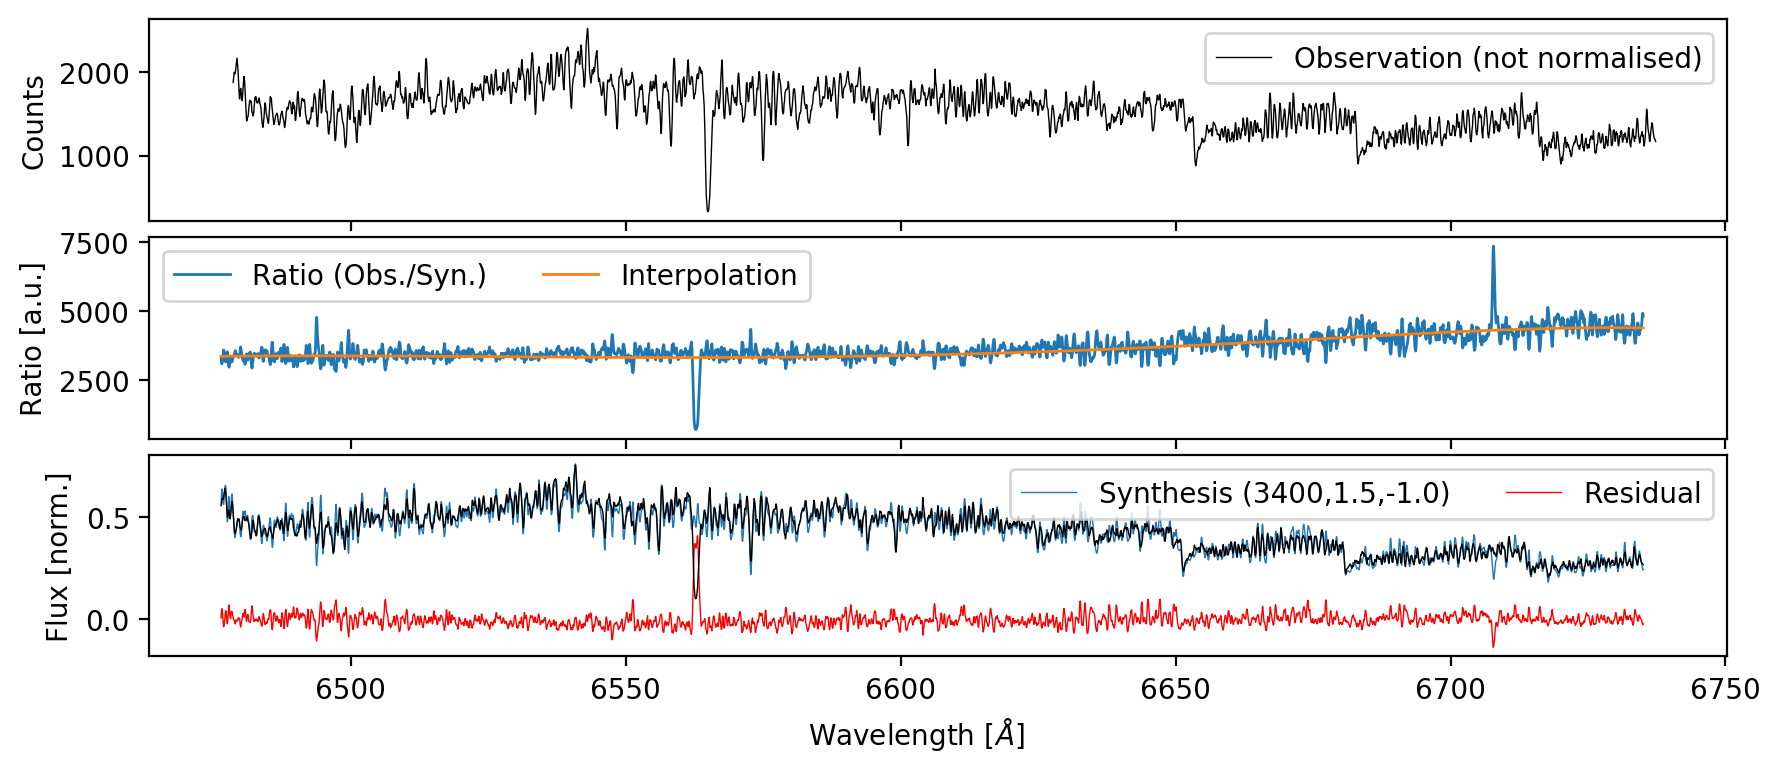
\includegraphics[width=\textwidth]{figures/Nuisance_example.png}
\caption{
\textbf{Example of normalisation for GALAH DR4 for a model spectrum that is selected during the label optimisation.}
\textbf{Panel (a):} Observed spectrum (counts).
\textbf{Panel (b):} Ratio (blue) of observed spectrum and model spectrum as well as Chebyshev polynomial fit (orange).
\textbf{Panel (c):} Normalised observed spectrum (black) compared to the model spectrum (blue). Residuals (red) can then be used as input for the likelihood function.
}
\label{fig:ratio_normalisation}
\end{figure}

As we compare the observation to model spectra, we do not have to restrict ourselves to an \textit{a priori} normalisation, but can take into account the residual information on the continuum in parts of the spectrum. For each model spectrum that we compare to, we therefore perform a normalisation by fitting a Chebyshev polynomial with outlier clipping to the ratio of model and observation (see Fig.~\ref{fig:ratio_normalisation}). This allows us to both overcome previous shortcomings of the synthetic analysis in GALAH+ DR3 \citep{Buder2021}, which had to be restricted to small wavelength segments and assumed a linear relation for those. Our new approach allows us to properly assess the structure of deep and steep molecular features that can dominate spectra of cool stars and carry significant information on \Teff as well as \vrad.

% \SB{Describe here the tests we do to make sure this actually provides a smooth transition between the different labels. Tests of the Cannon models show, that they can reproduce the spectra and their labels within for example $1\K$ \Teff, $0.01\dex$ \logg, and $0.01\dex$ \feh for the grid edges. But more thorough testing is needed.}
% \SB{Also keep in mind the issues found for \TheCannon with only 2 models applied to RAVE \citep{Casey2017}.}

%%%%%%%%%%%%%%%%%%%%%%%%%%%%%%%%%%%%%%%%%%%%%%%%%%%%%%%%%%%%%%%%%%%%%%%%%
\subsection{Stellar label optimisation}
\label{sec:stellar_label_optimisation}
%%%%%%%%%%%%%%%%%%%%%%%%%%%%%%%%%%%%%%%%%%%%%%%%%%%%%%%%%%%%%%%%%%%%%%%%%

In up to four major loops, we optimise the radial velocities and all other stellar labels and report a) their values, b) their co-variances, c) the best fit synthetic and re-normalised spectra along with d) their uncertainties and e) masks that indicate which pixels were used in the final optimisation.

Starting from the initial values, a first synthetic spectrum is computed and compared with the observation in order to assess the initial radial velocity. This is done by applying the \textsc{scipy.signal.find\_peaks} algorithm on the normalised inverse residuals of non-shifted observed and synthetic spectra, when the latter is shifted by $v_\text{rad} = -1000..(2)..1000\kms$ (see Fig.~\ref{fig:181221003101356_single_fit_rv}a). If no peak is found, the initial \vrad value is used hereafter. If more than one peak is found (see Fig.~\ref{fig:181221003101356_single_fit_rv} with \Gaia DR3 agreeing with the systemic radial velocity), the two strongest peaks are reported. For the purpose of the single star analysis, a narrower search is conducted around the highest peak with a \vrad shift of $-20.00..(0.04)..20.00\kms$ around said peak by fitting a Gaussian function to the inverse of the residuals that were normalised with the smallest residual values (see Fig.~\ref{fig:181221003101356_single_fit_rv}c). The mean of this fit and its uncertainty are reported by the pipeline.

\begin{figure}[hbt]
\centering
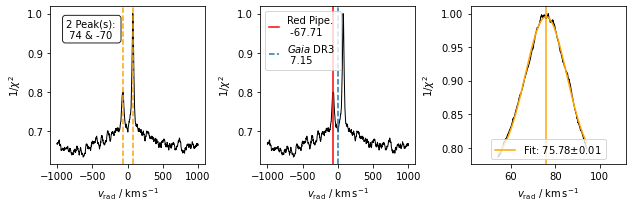
\includegraphics[width=\textwidth]{figures/181221003101356_single_fit_rv.png}
\caption{\textbf{Output of the radial velocity fitting module.} \textbf{Panel a)} shows the initial broad search on a \vrad array of $-1000..(2)..1000\kms$. In the case of 2MASS J06084657-7815235, two peaks (yellow, dashed) are visible for this double-lined spectroscopic binary. \textbf{Panel b)} shows the same plot, but overlaid with the GALAH DR4 reduction pipeline (red) and \Gaia DR3 (blue, dashed) estimates or \vrad. \textbf{Panel c)} shows the narrow window of $-20.00..(0.04)..20.00\kms$ around the highest peak and the Gaussian fit (yellow) to it.}
\label{fig:181221003101356_single_fit_rv}
\end{figure}

The centerpiece of our optimisation is the \textsc{scipy.optimise} module's \textsc{curve\_fit} function \citep{scipy}, which we call with counts and uncertainties (our absolute sigmas) as input for a placeholder function that self-consistently re-normalises the observed spectrum. We estimate the labels via the least squares optimisation within less than $10^4$ iterations and a desired relative error (\texttt{xtol}) below $10^{-4}$.

For the each optimisation loop, a new, best-fit 3D bin and neural network is identified via a grid search in the \TLF dimensions with \textsc{sklearn.cKDtree}. If the stellar labels that are being fitted have changed (for example if an element is deemed not detectable for the new 3D bin during the neural network training), the label and its value are either deleted or initialised with $\mathrm{[X/Fe]} = 0$.

While the optimisation has not converged (the final parameters \TLF are not within the current 3D bin), the optimisation is repeated, starting with the previous best-fit parameters as starting guesses.

\begin{figure*}[ht]
\centering  
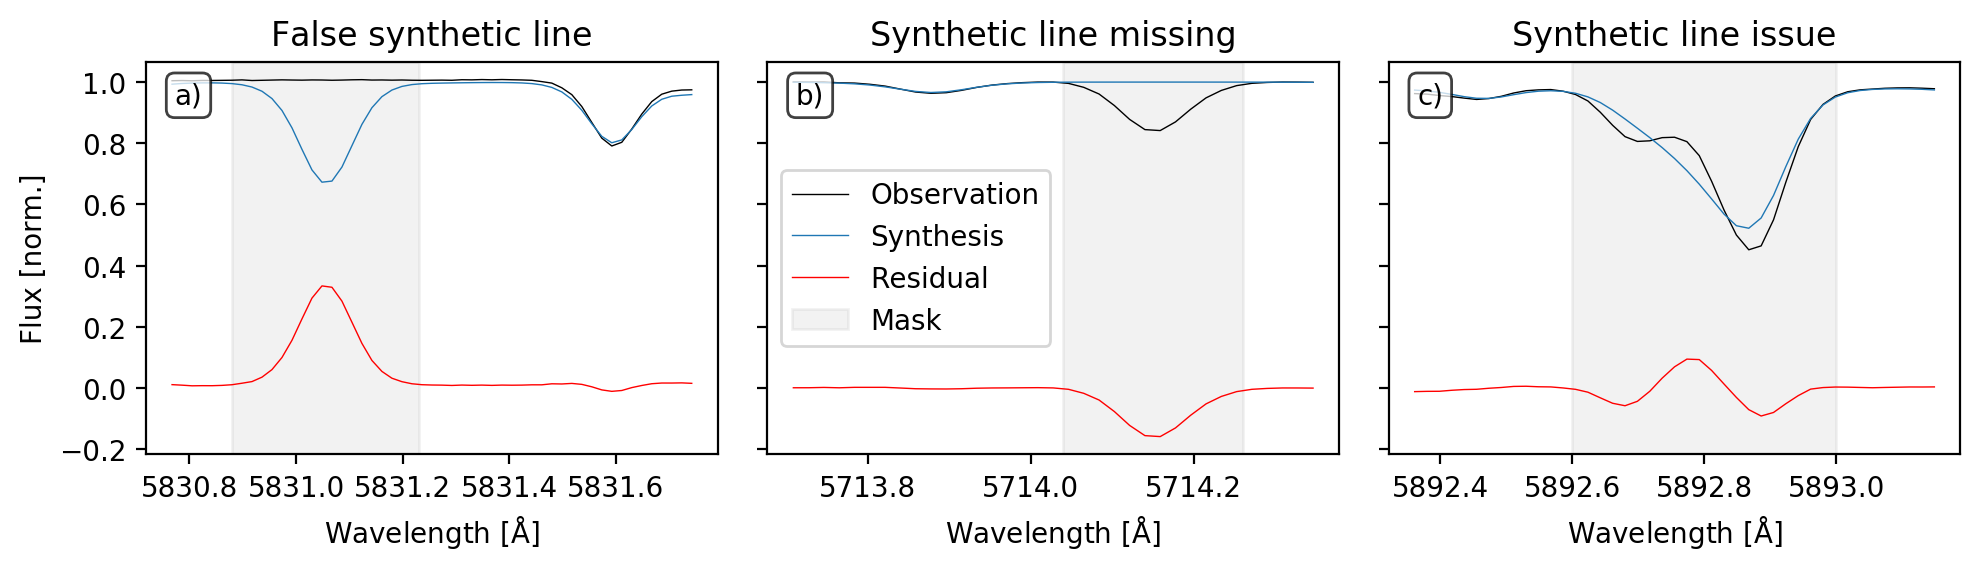
\includegraphics[width=\textwidth]{figures/example_masking_sun.png}
\caption{\textbf{Examples of masks applied to unreliable pixels for the spectrum fitting, which is done by the minimisation of residuals (red) between observation (black) and synthesis (blue).} \textbf{Panel a)} shows a strong synthetic line, where no line is observed in the data. \textbf{Panel b)} shows an observed line without any line being synthesised. \textbf{Panel c)} shows significant disagreement between the two observed lines and the synthesis.} \label{fig:example_masking_sun}
\end{figure*}

\subsubsection{Which labels are optimised?} \label{sec:which_labels_are_optimised}

%% This paragraph is based on the combination of 
%% spectrum_interpolation/galah_dr4_grid_interpolation_recommend_labels.ipynb
%% and
%% spectrum_analysis/galah_dr4_spectrum_analysis_single.ipynb

As part of the synthetic grid computations, we have perturbed each label individually to our chosen maximum and minimum ranges (see Sec.~\ref{sec:spectrum_grid}). This allows us to also judge which stellar labels to fit for each given star. We choose to fit a stellar label if either of these two cases applies to said label for the GALAH wavelength range when neglecting the cores of the Balmer lines: Does the spectrum between minimum and maximum label value at any pixel change more than a certain threshold (0.07 of the normalised spectrum)? Does the spectrum between minimum and maximum label value change by more than 0.005 of the normalised spectrum for at least 25\% of the spectrum? While the first case is constructed for atomic lines, such as \ion{Li}{i} 6708, the second case is addressing in particular molecular lines like the $\mathrm{C_2}$ and $\mathrm{CN}$ lines. For stars that are missing data from the infrared arm of HERMES (CCD4) we exclude the 
%otherwise possibly fit 
labels for N, O, L, and Rb.

Initial tests of the pipeline have revealed that in cases where the initial parameter estimates deviate significantly from the final values, several elemental abundance estimates were shifted towards their boundaries, leading to a masking of their elemental abundance lines by the masking module (Sec.~\ref{sec:masking_of_unreliable_wavelength_regions}) at the beginning of each optimisation loop. To minimise this effect, we therefore shift the interim abundance values towards the narrow label boundaries. In practise, we limit the initial and interim abundances to 1.05..3.26 for A(Li), $\mathrm{[X/Fe]} = -0.5..1.0$ for C, N, O, Y, Ba, La, Ce, and Nd, and $\mathrm{[X/Fe]} = -0.5..0.5$ for all other elements before optimising them again. For warm and hot stars ($T_\text{eff} > 6000\K$), this effect was seen to affect multiple abundances, such that we needed to implement a zeroing of all abundances except Li for stars above $6000\K$, which would on average be expected to be young and have a Solar-like composition.

\subsubsection{Masking of unreliable wavelength regions} \label{sec:masking_of_unreliable_wavelength_regions}

Not all pixels of the observed or synthetic spectra might prove useful for estimating reliable stellar labels. Observations can include bad pixels/patterns and incorrect corrections (for example of telluric or sky lines). Flux predictions of synthetic spectra are only as good as the input physics (limited for example for specific lines via uncertain oscillator strengths).

% Based on https://github.com/svenbuder/GALAH_DR4/blob/main/spectrum_analysis/galah_dr4_solar_analysis.ipynb
To minimise the influence of inaccurate synthetic pixel predictions, we have compared a 2dF-HERMES observation of the asteroid 4~Vesta and a high-quality Solar spectrum by \citet{Hinkle2000} with the flux that would be predicted through our pipeline for a star with Solar labels ($T_\text{eff} = 5772\K$, $\log g = 4.438\dex$, $\mathrm{[Fe/H]} = 0.00\dex$, $v_\text{mic} = 1.06\kms$, $v \sin i = 1.6\kms$, $v_\text{mac} = 4.2\kms$ \citep{Prsa2016, Jofre2017}, and $\mathrm{[X/Fe]} = 0.00\dex$ for the default Solar abundance pattern for \marcs by \citet{Grevesse2007}).

We have identified all lines that showed differences of the normalised flux of more than $0.1$, lines where either a synthetic line or an observed one was completely missing, or lines that were significantly misaligned. Examples of masks\footnote{See this \href{https://github.com/svenbuder/GALAH_DR4/blob/main/spectrum_analysis/spectrum_masks/solar_spectrum_mask.fits}{list}.} are shown in Fig.~\ref{fig:example_masking_sun}. To avoid the influence of bad spectrum regions with an observational origin, we mask pixels where the synthetic and re-normalised observed spectrum differ by more than $5\sigma$ or a flux of 0.3 (0.4 before the initial optimisation). To avoid the masking of lines that are vital for our spectroscopic analysis, we have created a list\footnote{The list is available under this\href{https://github.com/svenbuder/GALAH_DR4/blob/main/spectrum_analysis/spectrum_masks/vital_lines.fits}{link}.}  with segments of such lines that is mainly based on the previous element masks from GALAH DR3 \citep{Buder2021}. The final mask of pixels to use for the optimisation then includes all vital line regions, as well as those wavelengths that do not show a too strong disagreement between observation and synthesis and are not deemed unreliable in their synthesis.

In addition to this default masking, we exclude pixels for each major iteration, for which the flux of observation and synthesis differ by more than $5 \sigma$ and 30\% of the normalised flux and by more than 100\% of the normalised flux for the vital line regions.

We further indirectly take into account the currently less constrained molecular data for cool stars in optical spectra, in particular towards the blue \citep[e.g.][]{Rains2021}. For presumably cool stars (with initial $T_\text{eff} < 4100\,\mathrm{K}$), we therefore double the observational uncertainty of the blue arm.

%%%%%%%%%%%%%%%%%%%%%%%%%%%%%%%%%%%%%%%%%%%%%%%%%%%%%%%%%%%%%%%%%%%%%%%%%
\section{SINGLE STAR ANALYSIS (ALLSTAR)}
\label{sec:allstar_analysis}
%%%%%%%%%%%%%%%%%%%%%%%%%%%%%%%%%%%%%%%%%%%%%%%%%%%%%%%%%%%%%%%%%%%%%%%%%

After the \textit{allspec} module (Sec.~\ref{sec:allspec_analysis}) has been used to estimate spectroscopic labels for all spectra, we use the \textit{allstar} module to co-add spectra and analyse one spectrum per star while taking into account photometric and astrometric information to constrain the surface gravities. This approach was successfully applied for GALAH DR3 \citep{Buder2021}, using \Gaia DR2 distances \citep{BailerJones2018} to overcome spectroscopic degeneracies. For the co-adding, we test whether the radial velocity estimates of individual exposures agree within $2\sigma$. Below this threshold, we apply no radial velocity correction and fit a global radial velocity. Above this threshold (which is useful for single-lined spectroscopic binaries 
%of type 1 without line splitting 
as shown in Fig.~\ref{fig:examples_flag_sp_2}), we apply a radial velocity correction before co-adding.

\begin{figure}[ht]
 \centering
 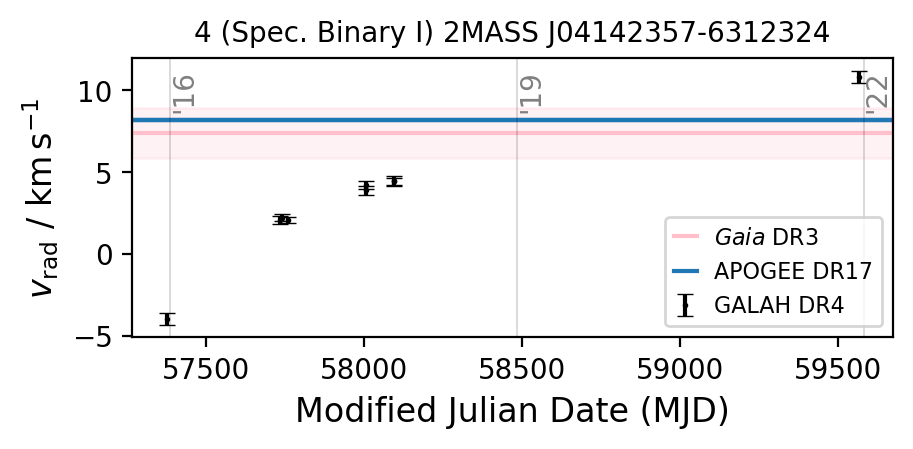
\includegraphics[width=\textwidth]{figures/examples_flag_sp_2.png}
 \caption{\textbf{Example of radial velocity evolution over time for a single-lined spectroscopic binary (SBI)}.}
 \label{fig:examples_flag_sp_2}
\end{figure}

To speed up computation, we use the mean results of the \textit{allspec} analyses as initial stellar labels for the \textit{allstar} analysis. All other methodology of the comparison of synthetic spectra to observations (Sec.~\ref{sec:comparison_synthetic_spectra_to_observations} and label optimisation (Sec.~\ref{sec:stellar_label_optimisation}) apply also to this module, with the exception of the optimisation of \logg. Contrary to the \textit{allspec} approach, we do not fit \logg in this module, but estimate the logarithmic surface gravity $\log g$ using a combination of its definition ($g \propto \frac{\mathcal{M}}{\mathcal{R}^2}$) and the Stefan-Boltzmann law relative to the Solar values:
\begin{equation}
\log g = \log g_\odot + \log \frac{\mathcal{M}}{\mathcal{M_\odot}} + 4 \log \frac{T_\mathrm{eff}}{T_\mathrm{eff,\odot}} - \log \frac{L_\mathrm{bol}}{L_\mathrm{bol,\odot}} \label{eq:logg}
\end{equation}

While we can use our spectroscopically determined $T_\mathrm{eff}$ in Eq. \ref{eq:logg}, the other values have to be estimated through models or non-spectroscopic information. The logarithmic bolometric luminosity, $L_\mathrm{bol}$, can be estimated from the bolometric magnitude, such that $\log \frac{L_\mathrm{bol}}{L_\mathrm{bol,\odot}} = -0.4 \cdot \left(M_\mathrm{bol} - M_\mathrm{bol,\odot} \right)$. The bolometric magnitude can be estimated from any given apparent magnitude, if we correct the latter by the distance modulus, bolometric correction, and extinction. Because essentially all stars in GALAH DR4 have outstanding infrared magnitudes available that suffer less from (uncertain) extinction corrections, we use $K_S$ as the magnitude to estimate our bolometric magnitudes and luminosities via
\begin{equation}
M_\mathrm{bol} = K_S - 5\cdot \log \frac{D_\varpi}{10} + BC(K_S) - A(K_S). \label{eq:mbol}
\end{equation}

While the values for $K_S$, $D_\varpi$, and $A(K_S)$ are readily available (see Sec.~\ref{sec:non-spec_data}), we need to estimate the bolometric correction from tabulated values using the routines provided by \citet{Casagrande2018}:
\begin{equation}
BC(K_S) = f(T_\mathrm{eff}, \log g, \mathrm{[Fe/H]})
\label{eq:bc_ks}
\end{equation}
We choose to assume an extinction value of $E(B-V) = 0\,\mathrm{mag}$ for this particular interpolation and post-correct the value by $A(K_S)$ based on the actual extinctions. The reason for this is that the latter values can exceed the maximum tabulated values of $E(B-V) = 0.72\,\mathrm{mag}$ by \citet{Casagrande2018}.

Because of the appearance of $\log g$ in Eq.~\ref{eq:bc_ks}, we iterate the calculation of $BC(K_S)$ and subsequently $\log g$ up to four times or until the latter value changes less than $0.02\,\mathrm{dex}$ between iterations. Similarly, we need to estimate the stellar masses (and ages as a byproduct) from tabulated values, that is,
\begin{equation}
\mathcal{M}, \tau = f(T_\mathrm{eff}, \log g, \mathrm{[Fe/H]}, L_\mathrm{bol,\odot})
\label{eq:mass_age}
\end{equation}
For this on-the-fly estimate of masses and ages we use an earlier version of the \texttt{ELLI} code by \cite{Lin2018} for a likelihood-weighted estimate with default uncertainties of $100\,\mathrm{K}$, $0.25\,\mathrm{dex}$, $0.2\,\mathrm{dex}$, and an average uncertainty of $L_\mathrm{bol,\odot}$ from propagated uncertainties of Eq.~\ref{eq:mbol}.

We interpolate over the default tables of {\sc parsec+colibri} isochrones \citep{Bressan2012, Marigo2017}, which cover the logarithmic ages of $\log (\tau~/~\mathrm{Gyr}) = 8.00..(0.01)..10.18$ by default and metallicities $\mathrm{[M/H]} = -2.75..(0.25)..-0.75$ as well as $\mathrm{[M/H]} = -0.6..(0.1)..0.7$. We exclude hot stars above $10\,000\,\mathrm{K}$ as well as extremely evolved white dwarf and extremely luminous giant stars ($\log g > 6\,\mathrm{dex}$ or $J - K_S > 2\,\mathrm{mag}$) as they fall far outside our spectroscopic pipeline range. We convert between the theoretical [M/H] and our measured [Fe/H] as well as an assumed $\mathrm{[\upalpha/Fe]}$ enhancement\footnote{We assume $\mathrm{[\upalpha/Fe]} = 0.4$ for $\mathrm{[Fe/H]} < -1$, $\mathrm{[\upalpha/Fe]} = 0.0$ for $\mathrm{[Fe/H]} > 0$ and linearly interpolate between these points for $-1 \leq \mathrm{[Fe/H]} \leq 0$.} via the correlation by \citet{Salaris2006}, $\mathrm{[M/H]} = \mathrm{[Fe/H]} + \log\left(10^{\mathrm{[\upalpha/Fe]}} \cdot 0.694 + 0.306 \right)$. For open clusters with age estimates below $1\,\mathrm{Gyr}$ as well as unevolved stars that are more luminous than expected from the oldest cool main sequence isochrone with matching $\mathrm{[M/H]}$, we sample $\log (\tau~/~\mathrm{Gyr}) = 6.19..(0.01)..10.18$. For globular cluster stars identified in the crossmatch with \citet{Baumgardt2021}, we limit the isochrones to a minimum age of $4.5\,\mathrm{Gyr}$.

\begin{figure*}[ht]
\centering
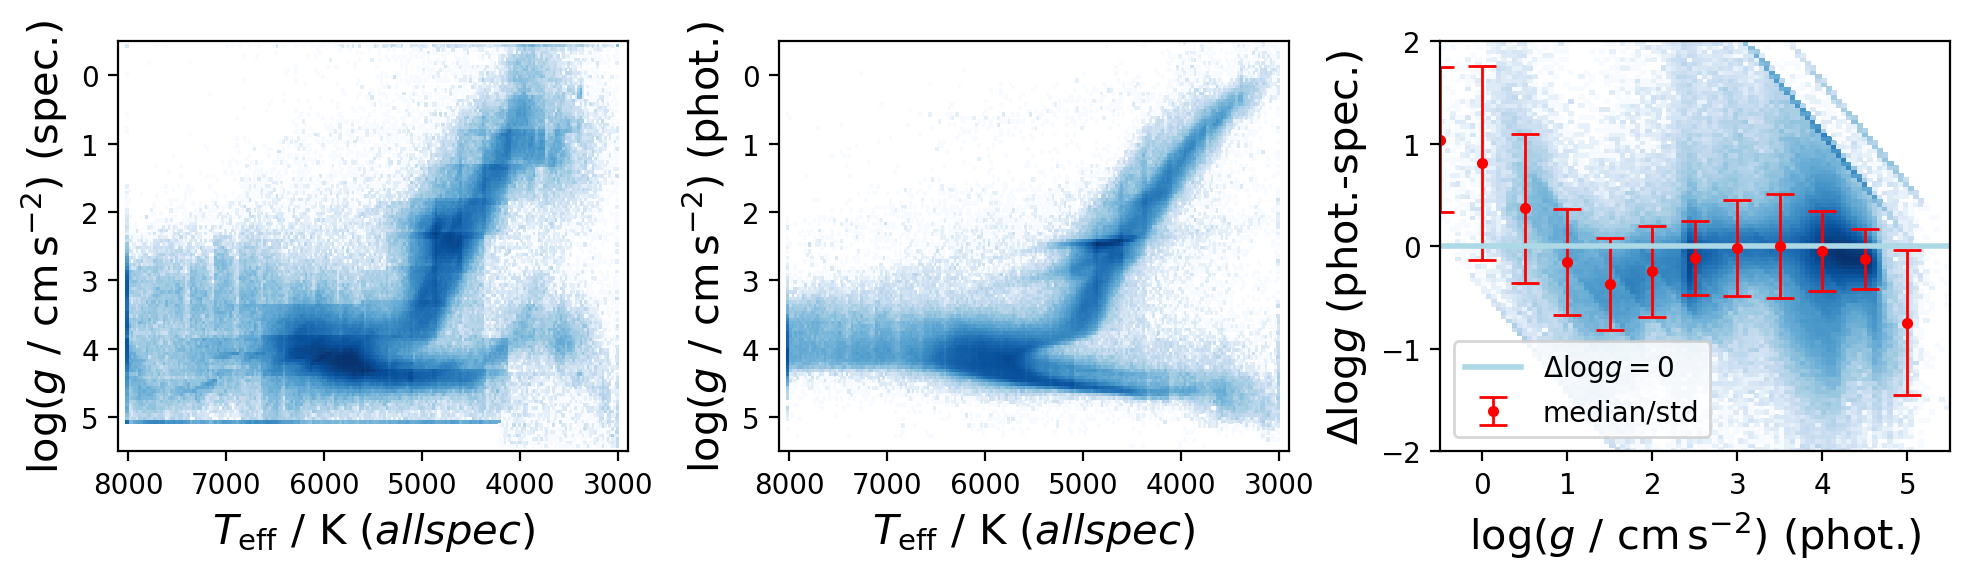
\includegraphics[width=\textwidth]{figures/dlogg_spec_plx.png}
\caption{\textbf{Comparison of spectroscopic and photometric \logg estimates in the \textit{allspec} analysis}
\textbf{Panel a)} shows the distribution of spectroscopic \logg and \Teff from the \textit{allspec} module.
\textbf{Panel b)} shows the distribution of the same \Teff and photometric \logg.
\textbf{Panel c)} shows the difference of photometric \logg and spectroscopic \logg as a function of photometric \logg. Red error bars indicate the $1\sigma$ percentiles of this difference in $0.5\,\mathrm{dex}$ bins.} \label{fig:dlogg_spec_plx}
\end{figure*}


%%%%%%%%%%%%%%%%%%%%%%%%%%%%%%%%%%%%%%%%%%%%%%%%%%%%%%%%%%%%%%%%%%%%%%%%%
\section{POST-PROCESSING}
\label{sec:post_processing}
%%%%%%%%%%%%%%%%%%%%%%%%%%%%%%%%%%%%%%%%%%%%%%%%%%%%%%%%%%%%%%%%%%%%%%%%%

After the \textit{allspec} (Sec.~\ref{sec:allspec_analysis}) and  \textit{allstar} (Sec.~\ref{sec:allstar_analysis}) modules have been run for a night's data, a post-processing routine is used to estimate additional parameters from the residuals of the spectra (Sec.~\ref{sec:residual_analysis}), estimate and validate accuracy and precision uncertainties (Sec.~\ref{sec:uncertainty}), and perform quality assurance tests on a global scale (\texttt{flag\_sp}, see Sec.~\ref{sec:flag_sp}) as well as for the individual abundances of elements X (\texttt{flag\_X\_fe}, see Sec.~\ref{sec:flag_x_fe}).

\subsection{Analysis of spectral residuals} \label{sec:residual_analysis}

\subsubsection{Binary signatures} \label{sec:trigger_binary_module}

The residual spectrum of our best fitting single star analysis can help us to identify a second flux contributor to the observed spectrum. In our case, there are two points in the analysis where we can identify such an influence. Firstly, the residuals are visible in the $\chi^2$ distribution as a function of radial velocity shifts (see Fig.~\ref{fig:181221003101356_single_fit_rv}). While a single star would only show one peak (saved as \texttt{rv\_comp\_1}), a binary system like 2MASS J06084657-7815235 shows a second peak ($-70\,\mathrm{km\,s^{-1}}$ in addition to $74\,\mathrm{km\,s^{-1}}$) that is saved as \texttt{rv\_comp\_2}. Secondly, we perform an automatic search for reoccuring residuals as a function of radial velocity for a few selected lines. We chose the combination of strong lines in the spectra (Balmer lines, Fe lines at 4890 and $4891\,\text{\AA}$, Ni at $6644\,\text{\AA}$) as well as those with the largest expected wavelength shift in the infrared detector (O triplet att $7772-7775\,\text{\AA}$ as well as Mg at $7692\,\text{\AA}$). If we find several peaks with a reasonably similar radial velocity, the likely $X \in {16,50,84}^\text{th}$ percentiles of this radial velocity are saved in \texttt{sb2\_rv\_X}.

Because radial velocities from the \Gaia radial velocity spectrometer \citep{Katz2022} are reported in \Gaia DR3 for 94\% (774\,914) of the stars observed for GALAH DR4, we can also compare against those radial velocity estimates. For 6\% (50\,577) of our stars, we find a difference with respect to \Gaia DR3 larger than $10\,\mathrm{km\,s^{-1}}$. For these stars, as well as stars for which we estimate unrealistic \vmic and \vsini below $0\,\mathrm{km\,s^{-1}}$ in \textit{allspec}. We note that the \textit{allspec} analysis was run without boundary conditions for global parameters and thus also resulted in negative velocities, which are later flagged. \textit{allstar}, however, was run with \vmic and \vsini forced to be above $0\,\mathrm{km\,s^{-1}}$.


\begin{figure*}[ht]
 \centering
 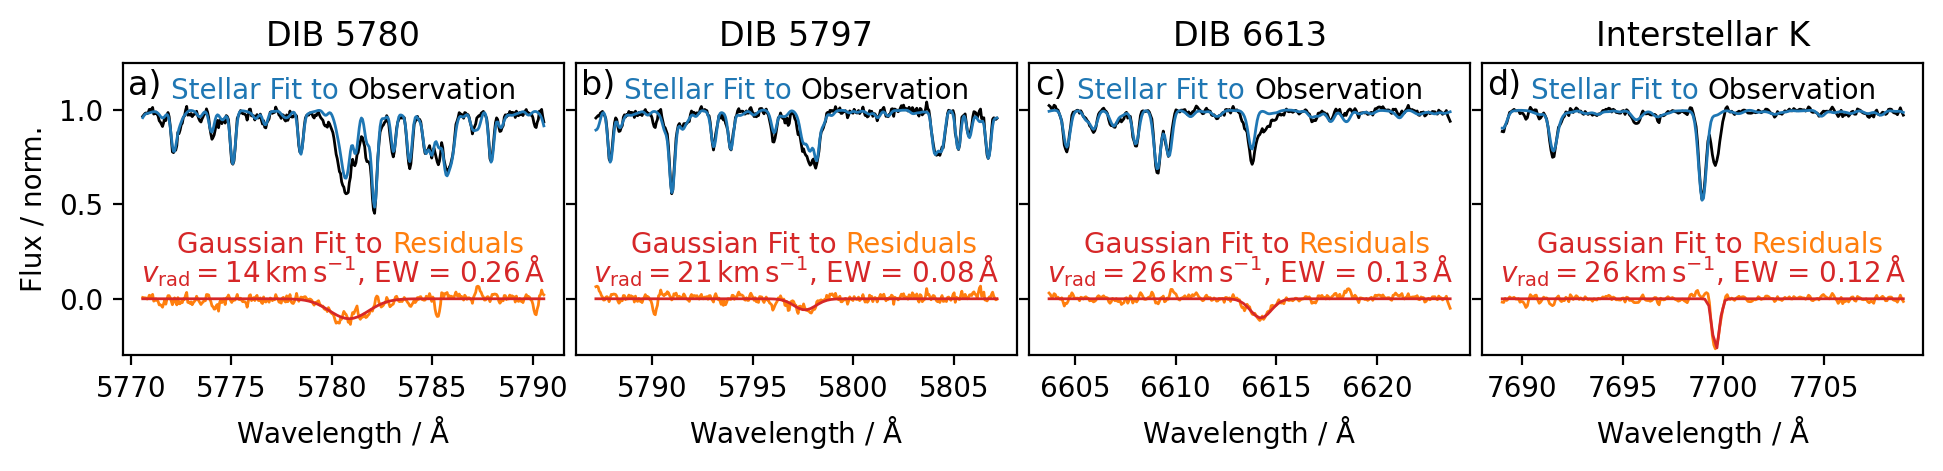
\includegraphics[width=\textwidth]{figures/example_dibs_06453479-0102137.png}
 \caption{\textbf{Example of three diffuse interstellar bands (DIBs) and interstellar K absorption for 2MASS J06453479-0102137 with an $E(B-V) = 0.84\,\mathrm{mag}$ value from \citet{Schlegel1998}.} Shown are the observation (black) and stellar fit (blue) as well as a Gaussian fit (red) to the residual (orange), resulting in an estimate of the equivalent width (EW) as well as radial velocity.} % 140314005201392
 \label{fig:example_dibs_06453479-0102137}
\end{figure*}

\subsubsection{Post-correction of {log\textit{g}} for \textit{allspec} results}

While we estimate logarithmic surface gravities \logg solely from spectra in the \textit{allspec} results, we also perform a post-processing estimate where we employ the methodology of Sec.~\ref{sec:allstar_analysis} while fixing all other stellar parameters. The approach of only using spectroscopic information confirmed the previous conclusions of GALAH DR1-DR3 that the spectroscopic information in HERMES spectra to estimate \logg is not sufficient for the majority of the parameter space for the given signal-to-noise. We show the spectroscopic \logg in Fig.~\ref{fig:dlogg_spec_plx}a and the photometric \logg and their difference in Figs.~\ref{fig:dlogg_spec_plx}b and c, respectively.

We see an overall good agreement of both \logg estimates for stars between $4250 < T_\text{eff} < 6500\,\mathrm{K}$. Hotter stars show a strong dispersion of spectroscopic \logg due to limited information from fewer and shallower lines. Cooler stars show a significant trend towards much lower \logg for main sequence stars and much higher \logg for cool evolved stars up to an order of $\Delta \log g$ of $1\,\mathrm{dex}$. This trend was previously seen in GALAH DR2 \citep{Buder2018} and is believed to be caused by the onset of molecular absorption features which suppress the continuum for almost the entire HERMES wavelength range (see for example Fig.~\ref{fig:ratio_normalisation}), thus introducing several degeneracies\footnote{\SB{Get back to this and include the private communication with Charlie Conroy on the \logg trends for cool stars.}}. In addition, we can notice a significantly lower precision of the spectroscopic \logg in comparison to the excellent precision of photometric \logg, for example in the red clump stars.

On closer inspection, we notice several trends in Fig.~\ref{fig:dlogg_spec_plx}a. Most notably, we see noding patterns along the \Teff and \logg grids where the \textit{allspec} module switches between different neural network models. Our investigation of these noding effects is addressed in Sec.~\ref{sec:caveats}. In comparison to Fig.~\ref{fig:dlogg_spec_plx}b, where a clear equal-mass binary sequence is visible just above the cool main sequence, we do not see such a sequence in Fig.~\ref{fig:dlogg_spec_plx}a. The difference between spectroscopic and photometric \logg will therefore be useful to identify photometric binaries at least for the high quality spectra (where \logg precisions are below the single to binary system offset of $\Delta \log g = 0.3\,\mathrm{dex}$), as discussed in Sec.~\ref{sec:flag_sp}.

\subsubsection{Interstellar absorption}

Because we can create synthetic stellar spectra for the full wavelength range, we can now also trace interstellar absorption in the residuals of observed spectra. By default, we try to calculate the equivalent width via Gaussian fits to the three diffuse interstellar bands (5780.59, 5797.19, 6613.66\Angstroem) with central wavelengths identified by \citet{Vogrincic2023} as well as for interstellar K ($7698.9643\,\text{\AA}$), see Fig.~\ref{fig:example_dibs_06453479-0102137}. We report the equivalent widths \texttt{eq\_x}, standard deviations \texttt{sigma\_x} and radial velocities \texttt{rv\_x} for \texttt{x} in \texttt{k\_is} for interstellar K and \texttt{x} in \texttt{DIB\_5780}, \texttt{DIB\_5797}, and \texttt{DIB\_6613} for the DIBs.

\subsubsection{Emission estimates for the Balmer lines}

The difference between synthetic and observed Balmer line absorption holds valuable information on active stars, as well as the known inaccuracy of the synthetic Balmer lines, as well as masses for evolved stars \citep{Bergemann2016} and possibly even information on unresolved binary systems \citep{Sayeed2024}. We therefore perform a trapezoidal integration around the Balmer lines at $4861.3230$ and $6562.7970\,\text{\AA}$ whose values we report in \texttt{ew\_h\_beta} and \texttt{ew\_h\_alpha}. By default we integrate in a window of $\pm 0.75$ and $1.25\,\text{\AA}$for $\text{H}_\beta$ and $\text{H}_\alpha$, respectively, and increase this window to $5\,\text{\AA}$ if the average observed, normalised flux within $\pm 0.5\,\text{\AA}$ of the Balmer line core exceeds 1. An example of such a star is shown in Fig.~\ref{fig:examples_flag_sp_1}, for which we measure a residual EW of $1.09\,\text{/AA}$.

\begin{figure}[ht]
 \centering
 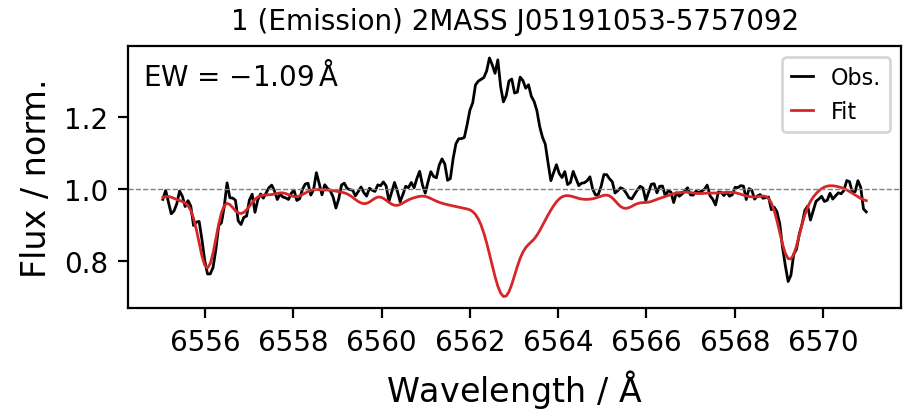
\includegraphics[width=\textwidth]{figures/examples_flag_sp_1.png}
 \caption{\textbf{Example of a star with clear emission in the Balmer lines (here $\mathrm{H_{\alpha}}$). The bit indicating emission has been raised in the major quality flag \texttt{flag\_sp} for this star.}} \label{fig:examples_flag_sp_1}
\end{figure}

\begin{figure}[ht]
 \centering
 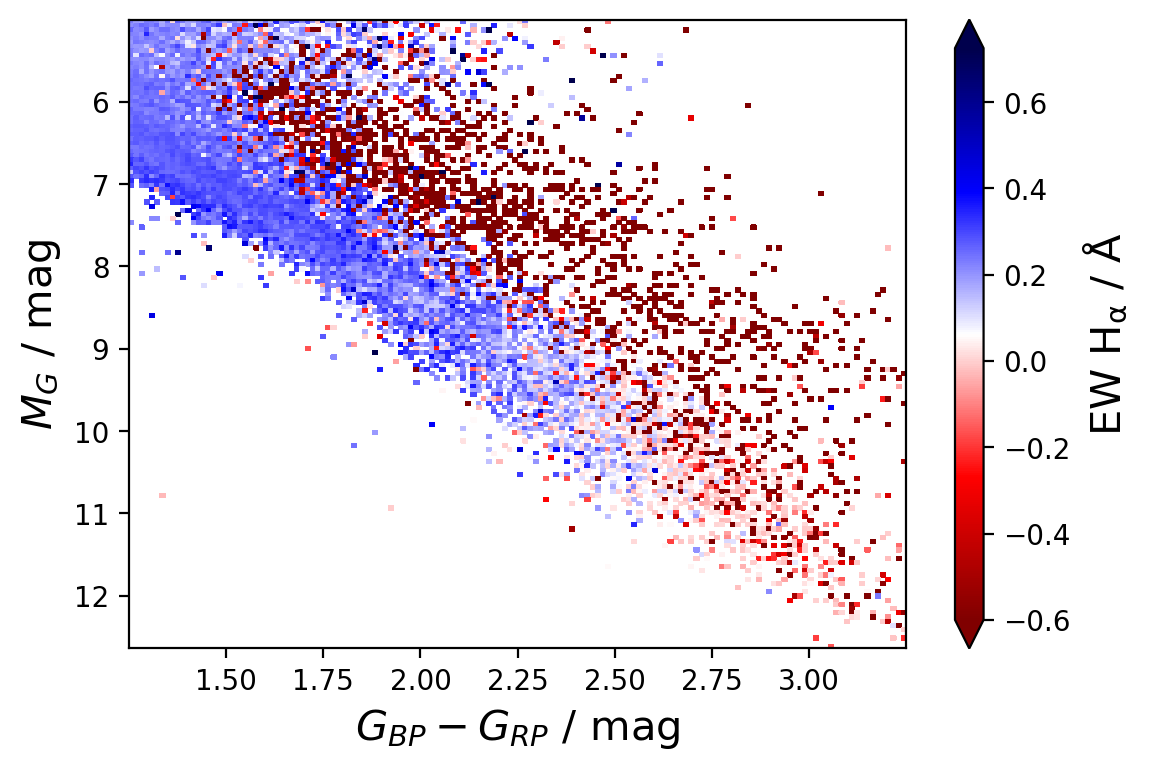
\includegraphics[width=\textwidth]{figures/emission_young_stars.png}
 \caption{\textbf{Distribution of residual equivalent width between observation and synthesis in the \Gaia DR3 color-absolute magnitude diagram ($G_{BP}-G_{RP}$ vs. $M_G$) for cool dwarfs.} Balmer lines in emission result in negative equivalent width values, as is the case for most young stars that are more luminous than the cool main sequence. \SB{Should we point out the interesting sequence of binary MS around $M_G \sim 7\,\mathrm{mag}$?}} \label{fig:emission_young_stars.png}
\end{figure}


%%%%%%%%%%%%%%%%%%%%%%%%%%%%%%%%%%%%%%%%%%%%%%%%%%%%%%%%%%%%%%%%%%%%%%%%%
\subsection{Uncertainty estimation and validation}
\label{sec:uncertainty}
%%%%%%%%%%%%%%%%%%%%%%%%%%%%%%%%%%%%%%%%%%%%%%%%%%%%%%%%%%%%%%%%%%%%%%%%%

The uncertainties that we report for our spectroscopic data analysis are based on the covariance matrix of the fitting process. While we report the covariance matrix for each spectrum (see Fig.~\ref{fig:covariance_vesta_arcturus} for the covariance matrices of Vesta and Arcturus), we restrict ourselves to the standard deviations of each feature (square root values of the diagonal variance entries).

\begin{table}
\centering
\caption{List of accuracy and representative precision uncertainties for stellar parameters in GALAH DR4. Accuracy values are estimated from comparisons with literature references (see Fig.~\ref{fig:galah_dr4_validation_parameter_accuracy_allstar}). Precision values are extracted from the median covariance uncertainties for stars with $SNR = 50 \pm 10$ in CCD2 (see Fig.~\ref{fig:galah_dr4_precision_parameters}).}
\label{tab:accuracy_precision}
\begin{tabular}{ccc}
\hline \hline
Parameter / Unit & Accuracy & Precision ($SNR = 50$)\\
\hline
$T_\text{eff}~/~\mathrm{K}$          & 66     & $23 \pm 5$ \\
$\log (g~/~\mathrm{cm\,s^{-2}})$     &  0.042 & -- \\
$\mathrm{[Fe/H]}~/~\mathrm{dex}$     &  0.051 & $0.025 \pm 0.004$ \\
$v_\text{mic}~/~\mathrm{km\,s^{-1}}$ &  0.28  & $0.05 \pm 0.03$ \\
$v \sin i~/~\mathrm{km\,s^{-1}}$     &  1.4   & $0.5 \pm 0.2$ \\
$v_\text{rad}~/~\mathrm{km\,s^{-1}}$ &  0.15  & $0.17 \pm 0.02$ \\
\hline
\end{tabular}
\end{table}

\subsubsection{Accuracy estimation and validation} \label{sec:uncertainty_accuracy}

Estimating the accuracy of spectroscopic measurements has always been a complicated endeavour, because there are no universal benchmark sets for all parameters. Subsequently, we there describe the numerous comparisons that we have performed for both stellar parameters (\Teff, \logg, \feh, \vmic, \vsini, and \vrad) as well as the elemental abundance measurements. Due to the limited coverage of benchmark literature, we continue to apply a universal accuracy estimate for the stellar parameters and no accuracy estimate for the elemental abundances \citep[as for GALAH DR3][]{Buder2021}.

% \SB{Describe shifts applied to the parameters and abundances. Most important is the increase of $\mathrm{[Fe/H]}$: Here we had to apply a piece-wise shift, described in Eq.~\ref{eq:piecewise_feh_shift}}
% \begin{align}
% \Delta \mathrm{[Fe/H]}=
% \begin{cases}
% 0.049 \qquad &\mathrm{for~[Fe/H]} \geq 0,\\
% 0.149 \qquad &\mathrm{for~[Fe/H]} \leq -1,\\
% 0.049 - 0.1 \cdot \mathrm{[Fe/H]} \qquad &\text{else}\\
% \end{cases} \label{eq:piecewise_feh_shift}
% \end{align}

\begin{figure*}[ht]
 \centering
 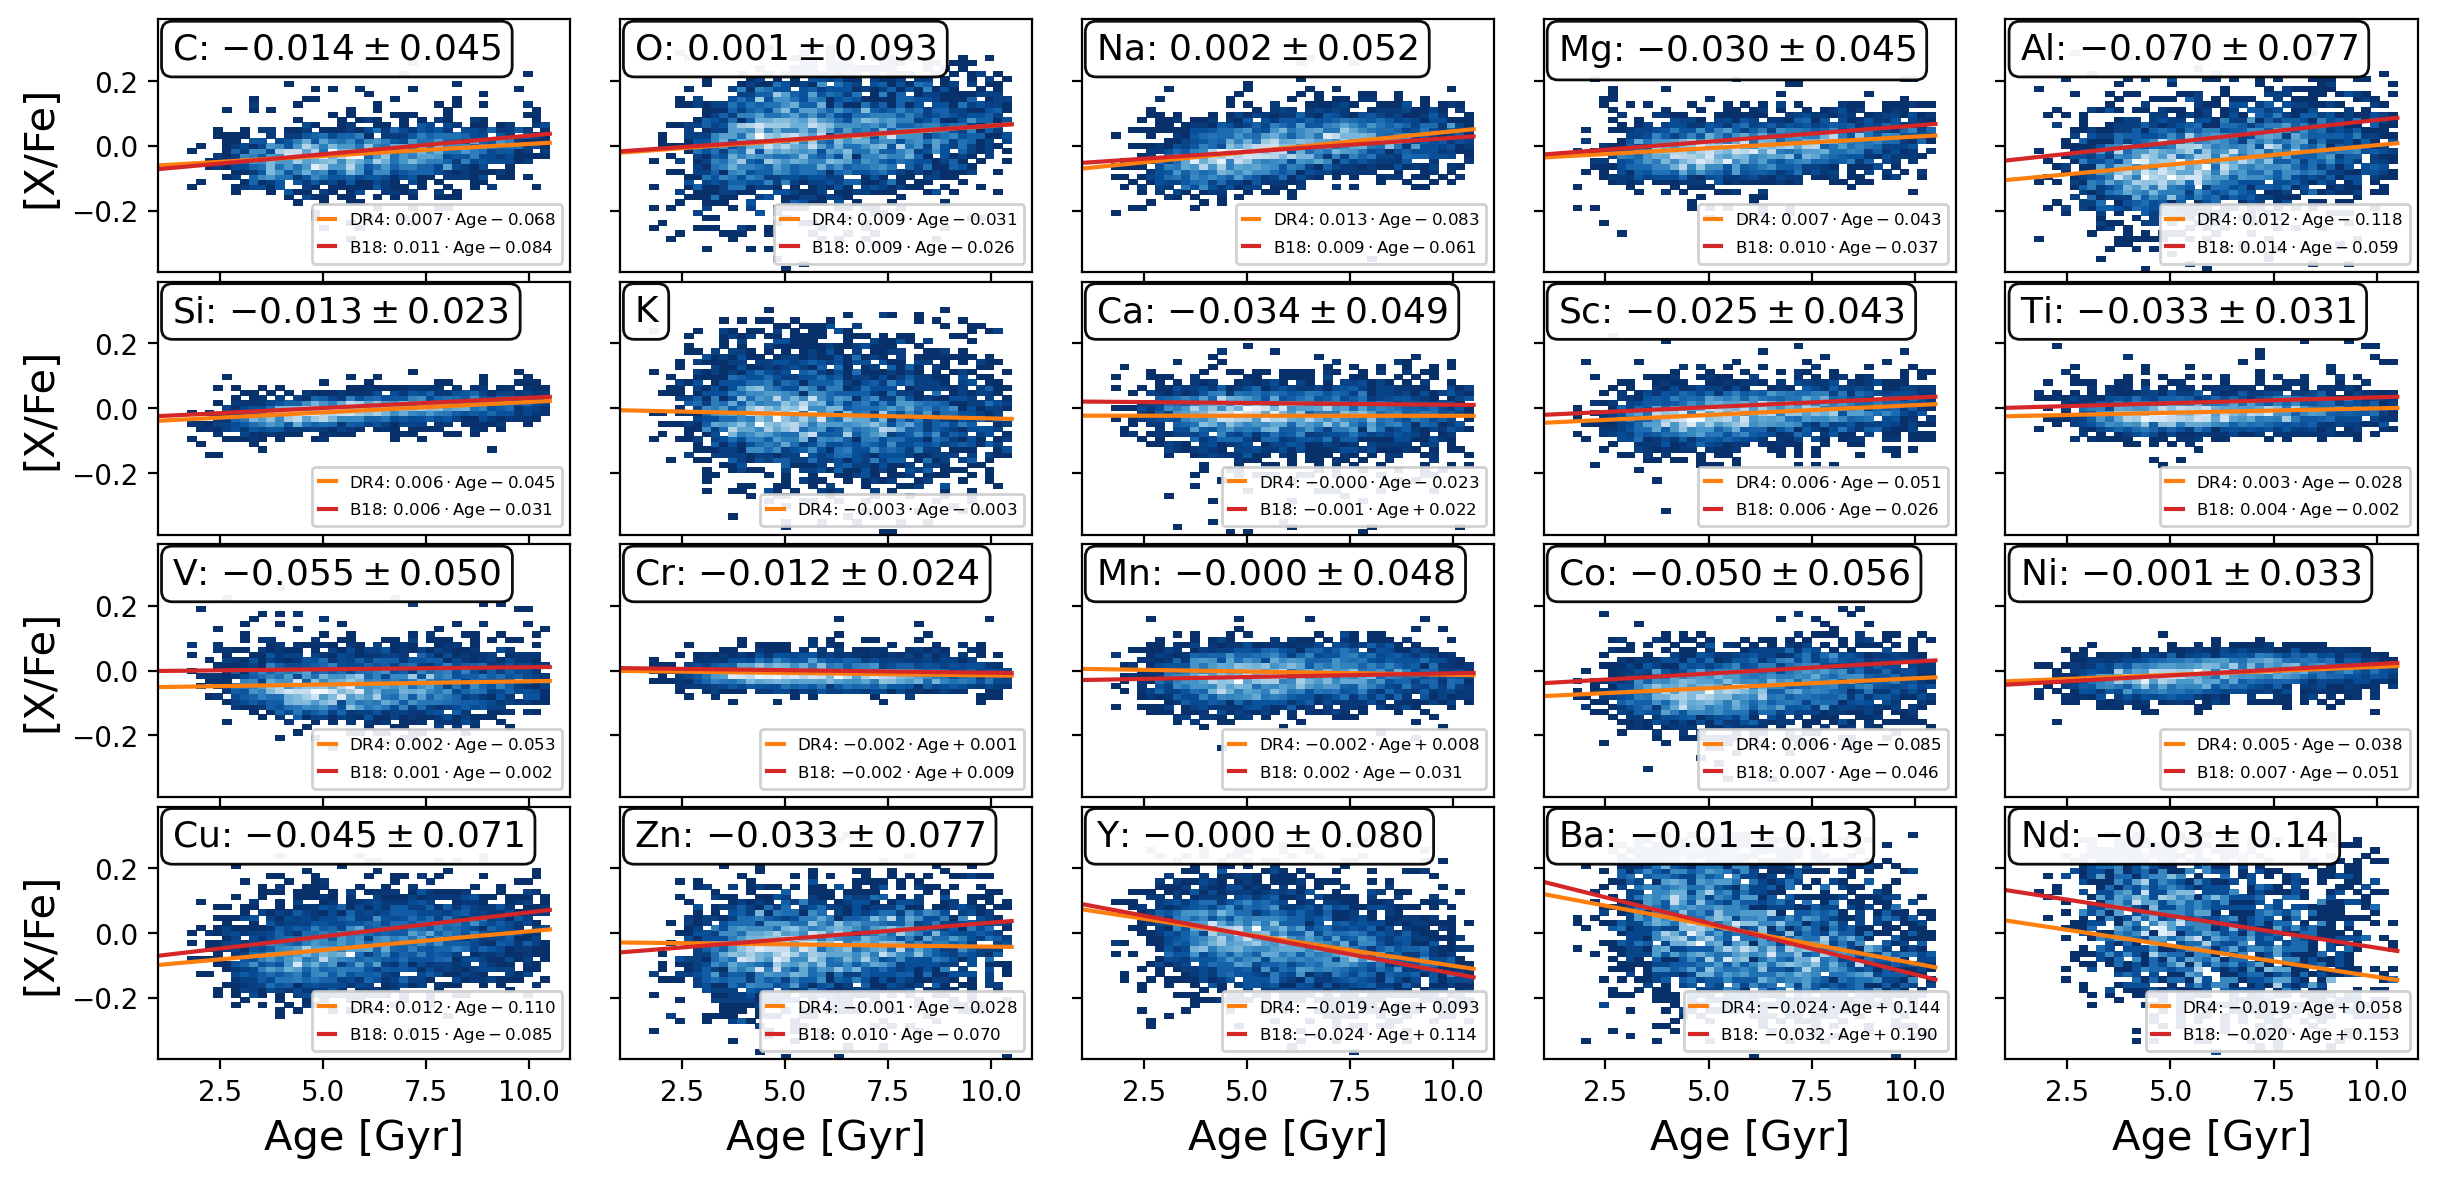
\includegraphics[width=\textwidth]{figures/galah_dr4_age_xfe_trends_solar_twins_allstar.png}
 \caption{\textbf{Chemical abundances [X/Fe] of Solar twin stars as a function of ages that were estimated as part of the mass and age estimation of the allstar spectrum analysis.} We overplot linear fits to our age-abundance relations for Solar twins in orange as well as the literature values from \citet{Bedell2018} in red.}
 \label{fig:galah_dr4_age_xfe_trends_solar_twins_allstar}
\end{figure*}


% \SB{Still to Do: Wide Binaries for Fig.~\ref{fig:galah_dr4_zeropoint_checks_allstar}}

Fig.~\ref{fig:galah_dr4_validation_parameter_accuracy_allstar} for stellar parameters and Fig.~\ref{fig:galah_dr4_zeropoint_checks_allstar} for abundances.

\begin{figure*}[ht]
 \centering
 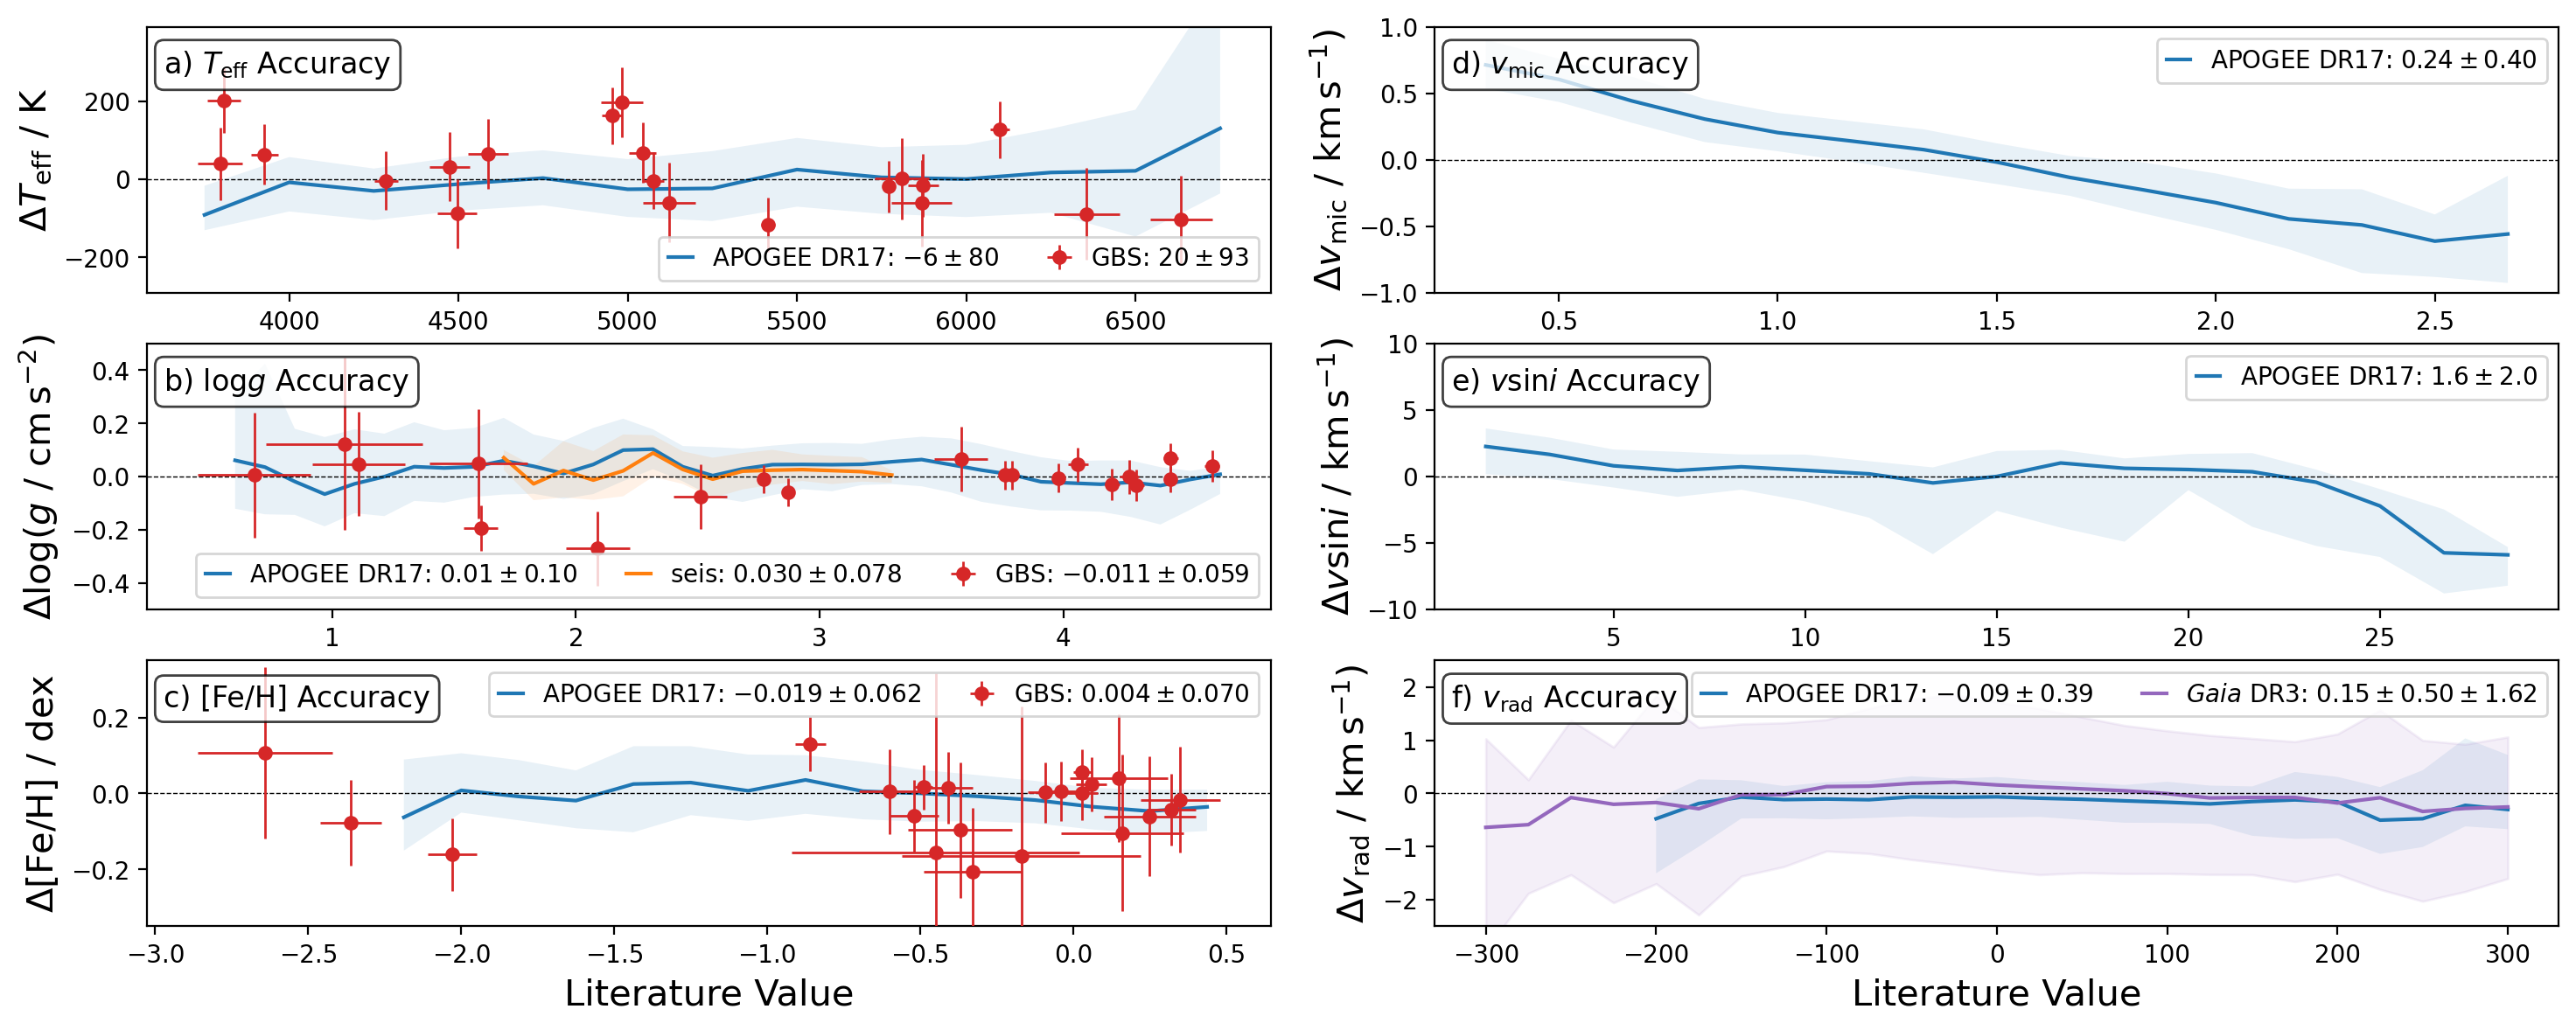
\includegraphics[width=\textwidth]{figures/galah_dr4_validation_parameter_accuracy_allstar.png}
 \caption{\textbf{Accuracy of the main stellar parameters \Teff, \logg, \feh, \vmic, \vsini, and \vrad for GALAH DR4.}. Each panel shows the comparison to literature (DR4 - literature). Comparisons are performed for the \Gaia FGK Benchmark stars (red), APOGEE DR17 (blue), \logg inferred from asteroseismic measurements (orange) and \Gaia DR3 radial velocities (purple).}
 \label{fig:galah_dr4_validation_parameter_accuracy_allstar}
\end{figure*}

\begin{figure*}[ht]
 \centering
 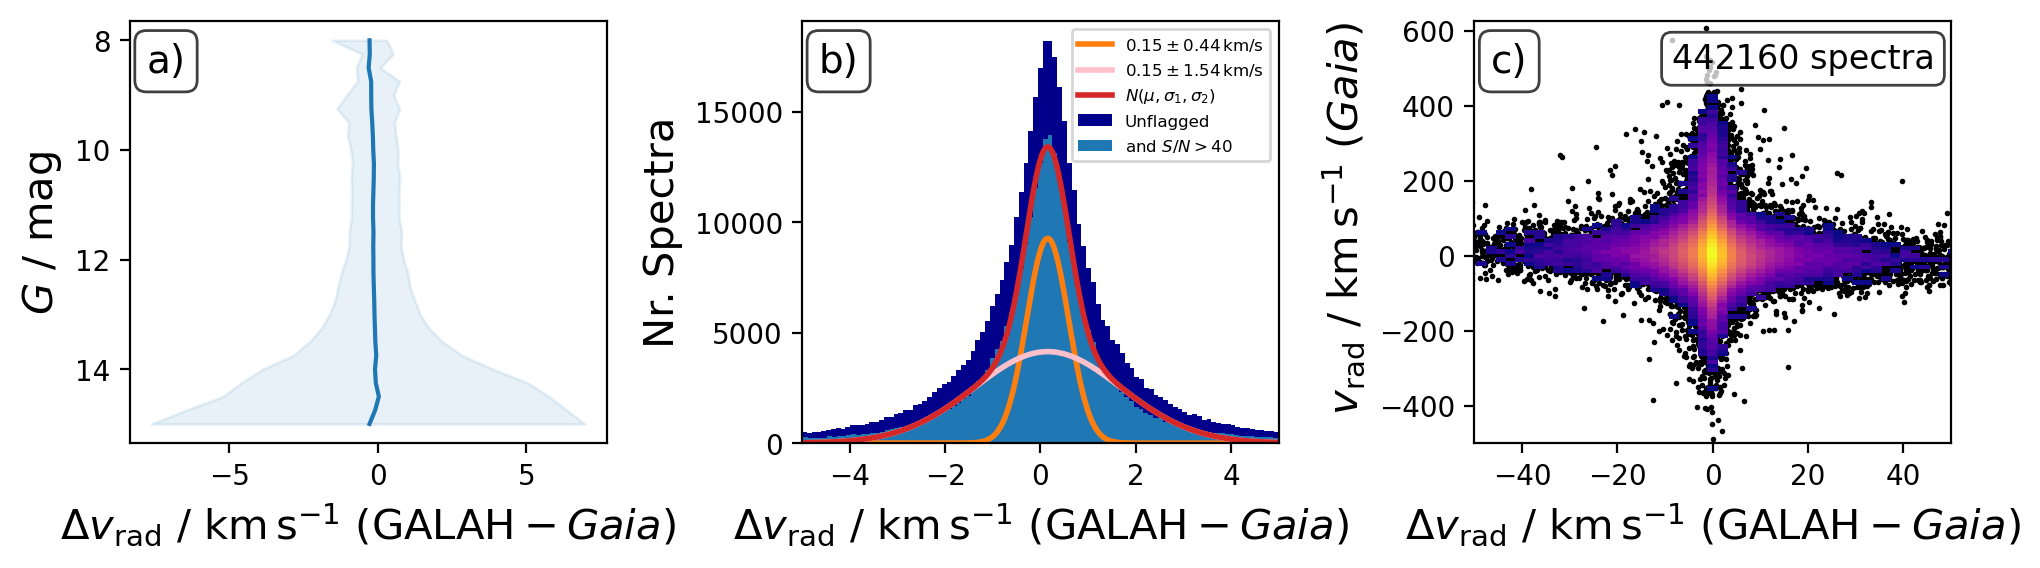
\includegraphics[width=\textwidth]{figures/galah_dr4_vrad_gaia_dr3.png}
 \caption{\textbf{Comparison of radial velocities between GALAH DR4 and \Gaia DR3.}
 \textbf{Panel a)} shows the difference of radial velocities as function of \Gaia $G$ magnitude.
 \textbf{Panel b)} shows a histogram of the difference with two Gaussian distributions (with same mean) fitted to them to estimate a more robust, that is binary independent, radial velocity difference.
 \textbf{Panel c)} shows the difference of radial velocities as function of radial velocity, showing the systematic scatter introduced by binaries.
}
 \label{fig:galah_dr4_vrad_gaia_dr3}
\end{figure*}


\begin{figure}
 \centering
 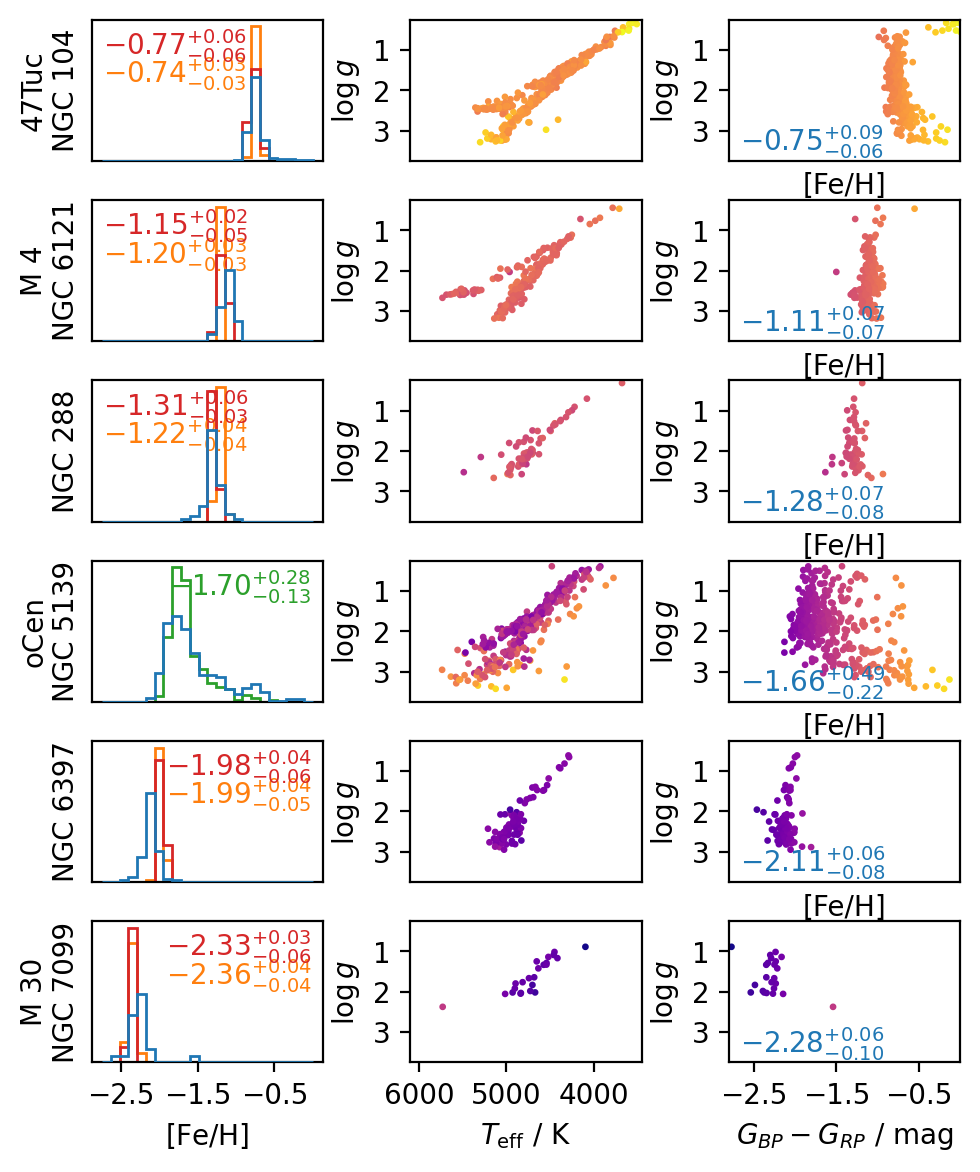
\includegraphics[width=\textwidth]{figures/galah_dr4_allstar_globular_cluster_feh_comparison.png}
 \caption{\textbf{Comparison of iron abundances (16th, 50th and 84th percentiles) and overview of spectroscopic and photometric properties of globular cluster stars in GALAH DR4.}
 \textbf{Left panels} show histograms of iron abundances from GALAH DR4 (blue) as well as literature estimates for the globular clusters from Giraffe (orange) and UVES (red) observations by \citep{Carretta2009, Carretta2009c} as well as observations from \cite{Johnson2010}.
 \textbf{Middle panels} show the spectroscopic \Teff-\logg diagrams colored by iron abundance \feh.
 \textbf{Right panels} show the \Gaia DR3 color absolute magnitude diagrams.
}
 \label{fig:galah_dr4_allstar_globular_cluster_feh_comparison}
\end{figure}


\begin{figure*}[ht]
 \centering
 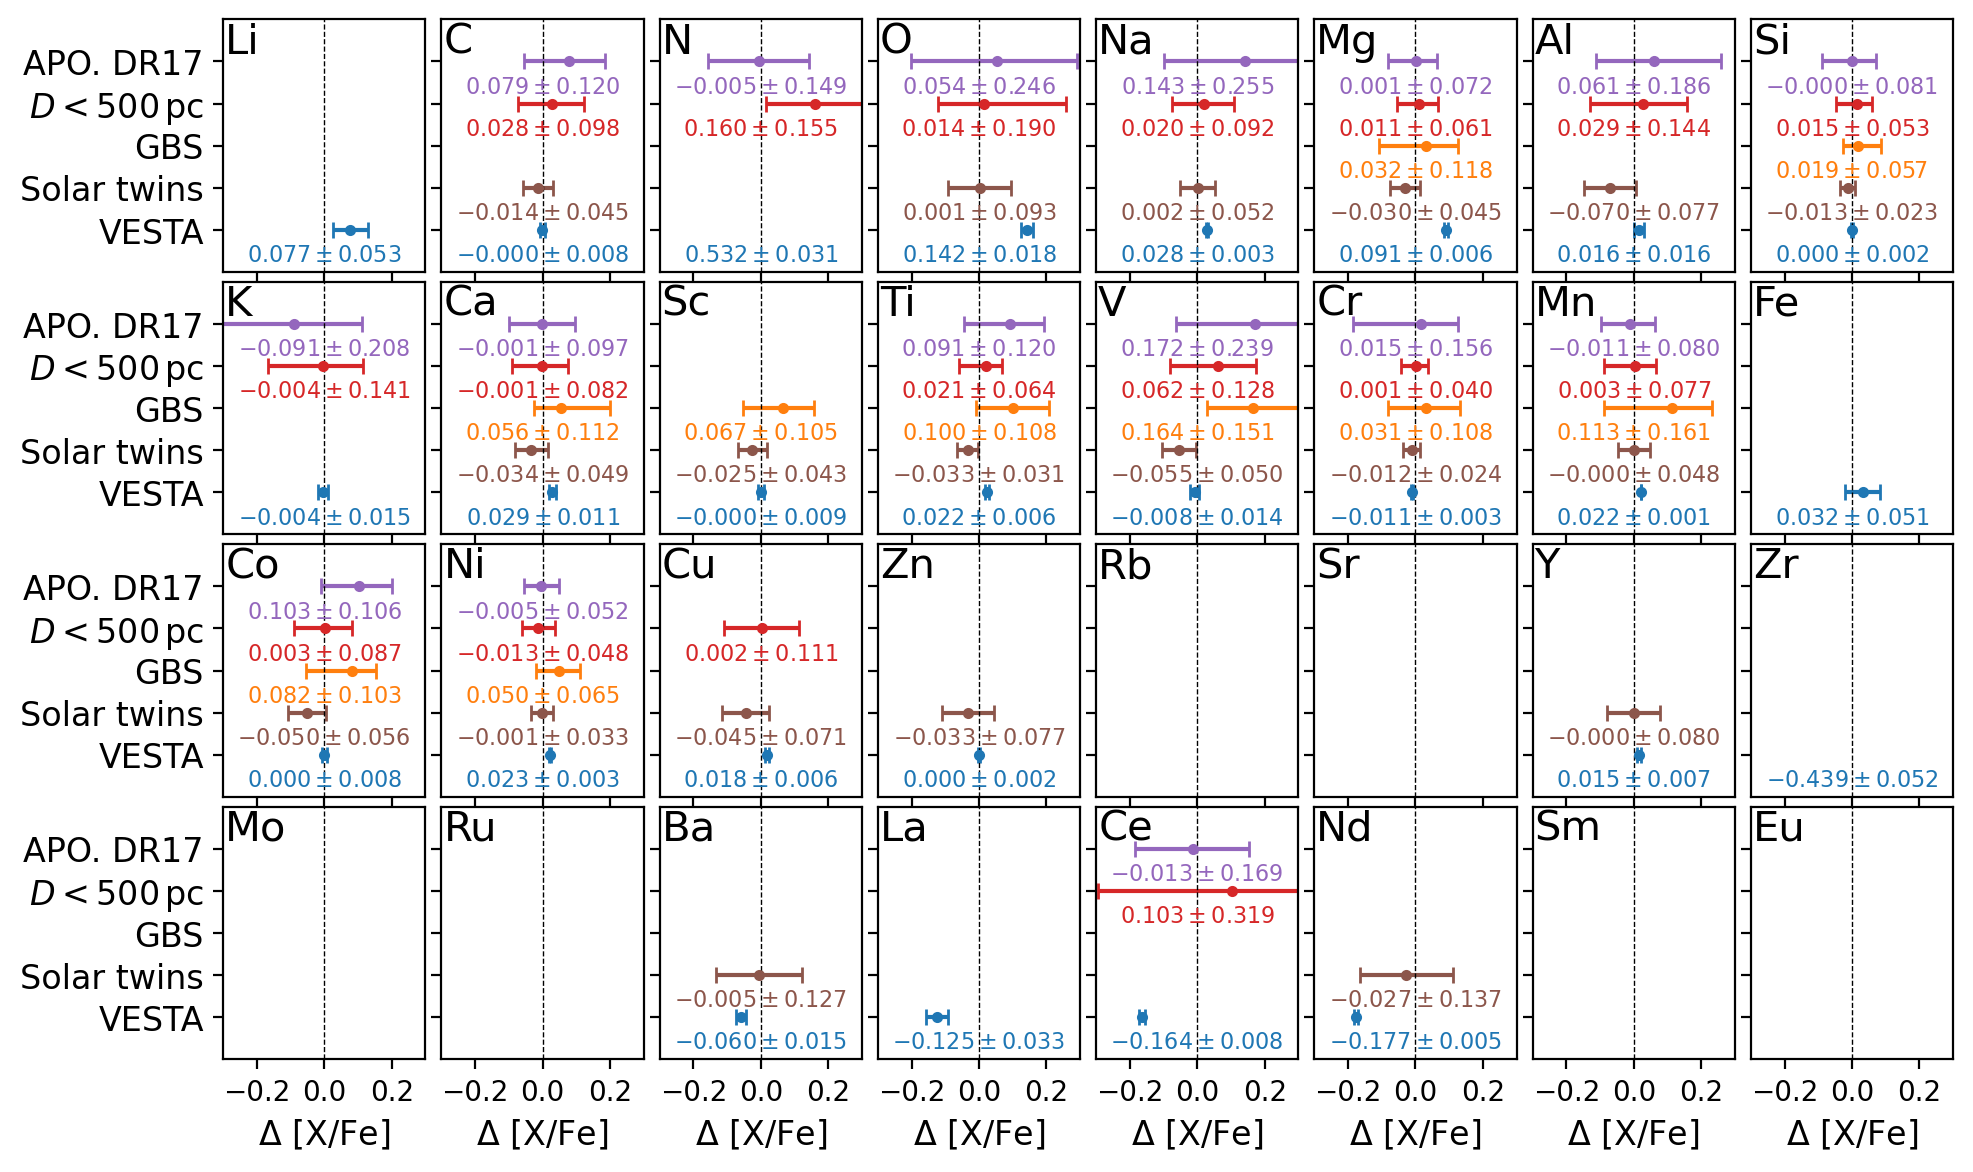
\includegraphics[width=\textwidth]{figures/galah_dr4_zeropoint_checks_allstar.png}
 \caption{\textbf{Zeropoint estimates of elemental abundances for GALAH DR4.}. Each panel shows the comparison to literature (DR4 - literature) for Vesta (blue), \Gaia FKG Benchmark Stars (orange), Stars with $\vert \mathrm{[Fe/H]} \vert \leq 0.1$ closer than $D_\varpi < 0.5\,\mathrm{kpc}$ (red), as well as stars that were also observed by APOGEE DR17 (purple).}
 \label{fig:galah_dr4_zeropoint_checks_allstar}
\end{figure*}

\begin{itemize}
    \item \Gaia FGK Benchmark stars \citep{Jofre2018} Fig.~\ref{fig:galah_dr4_validation_parameter_accuracy_allstar}a-c
    \item IRFM \citep{Casagrande2020}
    \item K2/TESS \citet{Zinn2020} Fig.~\ref{fig:galah_dr4_validation_parameter_accuracy_allstar}b
    \item APOGEE DR17 Fig.~\ref{fig:galah_dr4_validation_parameter_accuracy_allstar}a-f
    \item \Gaia DR3 for \vrad Fig.~\ref{fig:galah_dr4_validation_parameter_accuracy_allstar}f
    \item Globular Clusters for low \feh accuracy Fig.~\ref{fig:galah_dr4_gcs_teff_logg}
    \begin{itemize}
        \item 47 Tuc \citet{Carretta2009, Carretta2009b}
        \item NGC 6362
        \item M4
        \item NGC 362 \citet{Monty2023}?
        \item NGC 288 \citet{Monty2023}?
        \item NGC 1851
        \item M2 NGC 7089, with 3 populations in \feh according to \citet{Yong2014}. 21331790-0048198 was even observed by \citet{Yong2014} as NR 79 / HI-104 with $\mathrm{[Fe/H]} = -1.69$. We get $-1.37 \pm 0.26$, but at SNR around 10.
        \item Omega Cen \cite{Johnson2010}
        \item NGC 6397 \citet{Carretta2009, Carretta2009b}
        \item M30 \citet{Carretta2009, Carretta2009b}
    \end{itemize}
    \item Abundance Zeropoints
    \begin{itemize}
        \item Vesta
        \item APOGEE DR17
        \item Solar twins
        \item  M~67, Ruprecht~147 and a few others cover stars across several evolutionary stages. Check them roughly (could also be problematic because of atomic diffusion etc.)
    \end{itemize}
\end{itemize}

\begin{landscape}
\begin{figure}
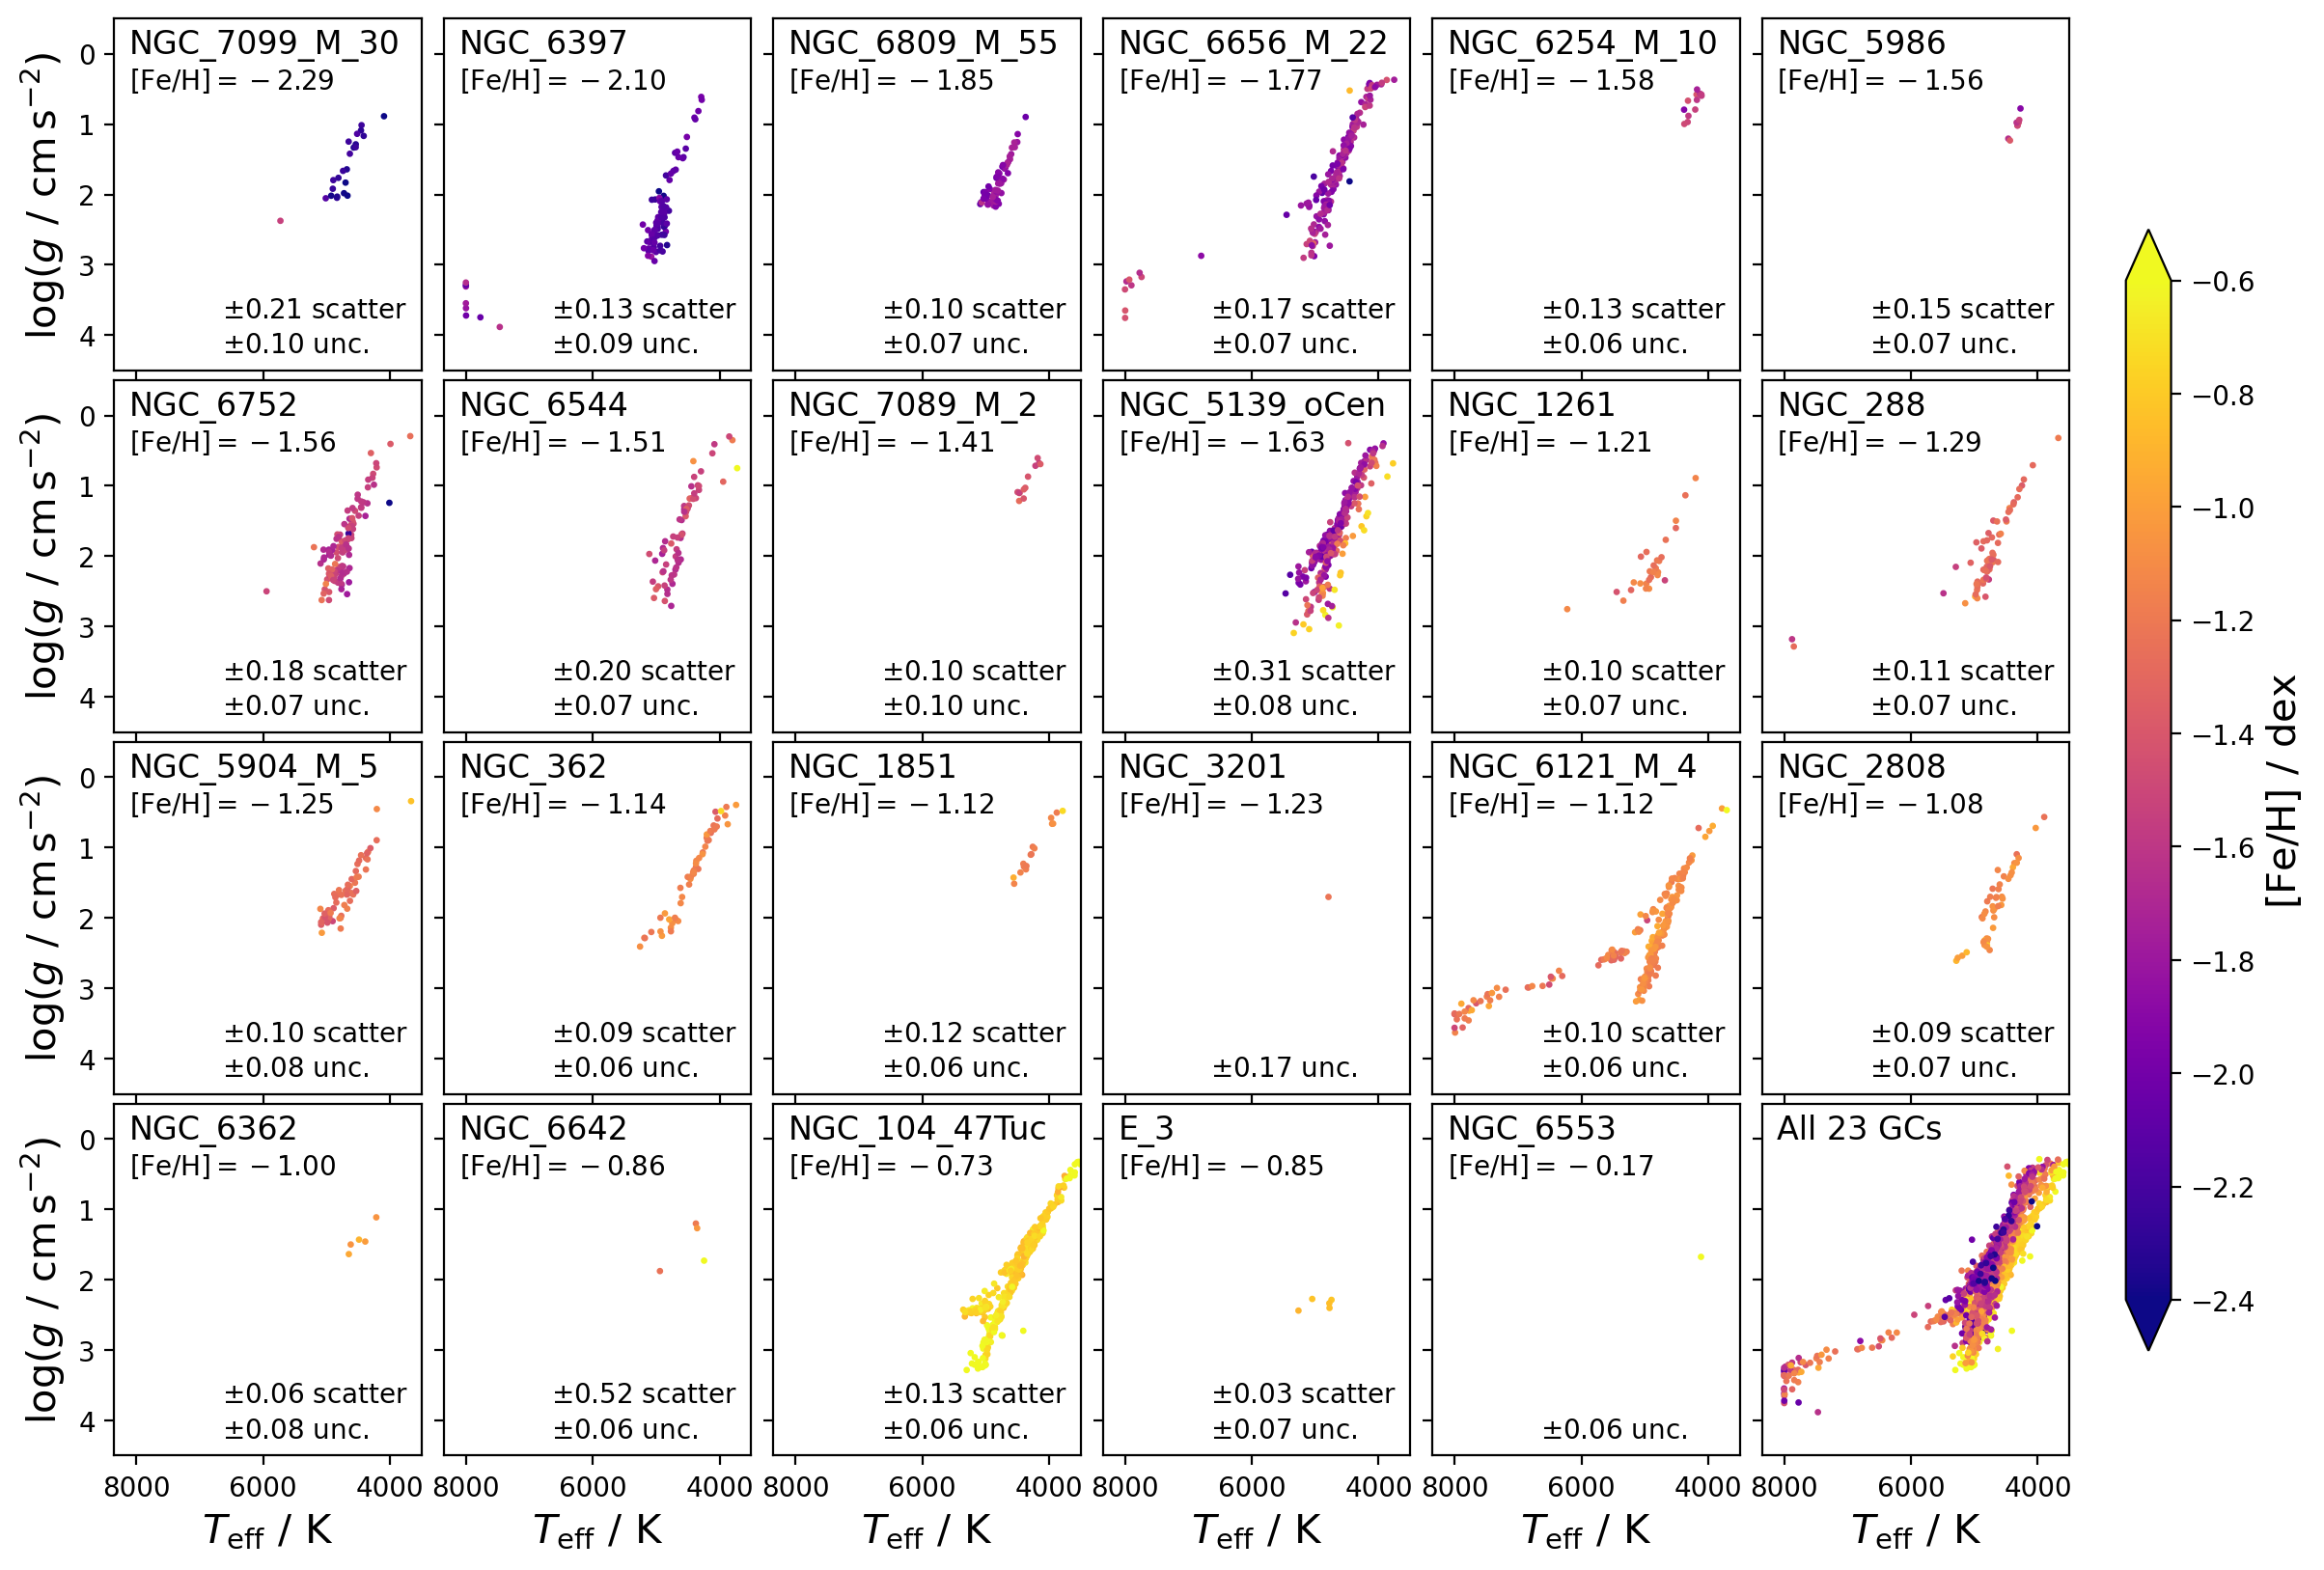
\includegraphics[width=0.975\columnwidth]{figures/galah_dr4_gcs_teff_logg.png}
\caption{
\textbf{Collage of globular clusters in the \Teff-\logg space, coloured by stellar metallicity \feh.} There are no strong systematic trends between \feh and \Teff, even for the horizontal branch stars in NGC 288, NGC 6656 (M22), and NGC 6121 (M4). NGC 5139 ($\mathrm{\omega}$Cen) shows a significant range in \feh. RMS scatter and median metallicity uncertainties for each cluster are given in the lower right of each panel. Most other clusters are consistent with no metallicity spread beyond the measurement uncertainties. 
}
\label{fig:galah_dr4_gcs_teff_logg}
\end{figure}
\end{landscape}


\subsubsection{Precision estimation and validation} \label{sec:uncertainty_precision}

\begin{itemize}
    \item Fig.~\ref{fig:galah_dr4_precision_parameters} and \ref{fig:galah_dr4_precision_abundances}
    \item \SB{Create Table with overall scatter values for individual elements based on:}
    \item Covariance uncertainties
    \item Repeat observations
    \item Scatter in open clusters
    \item Wide binary scatter
\end{itemize}

\begin{figure}[ht]
 \centering
 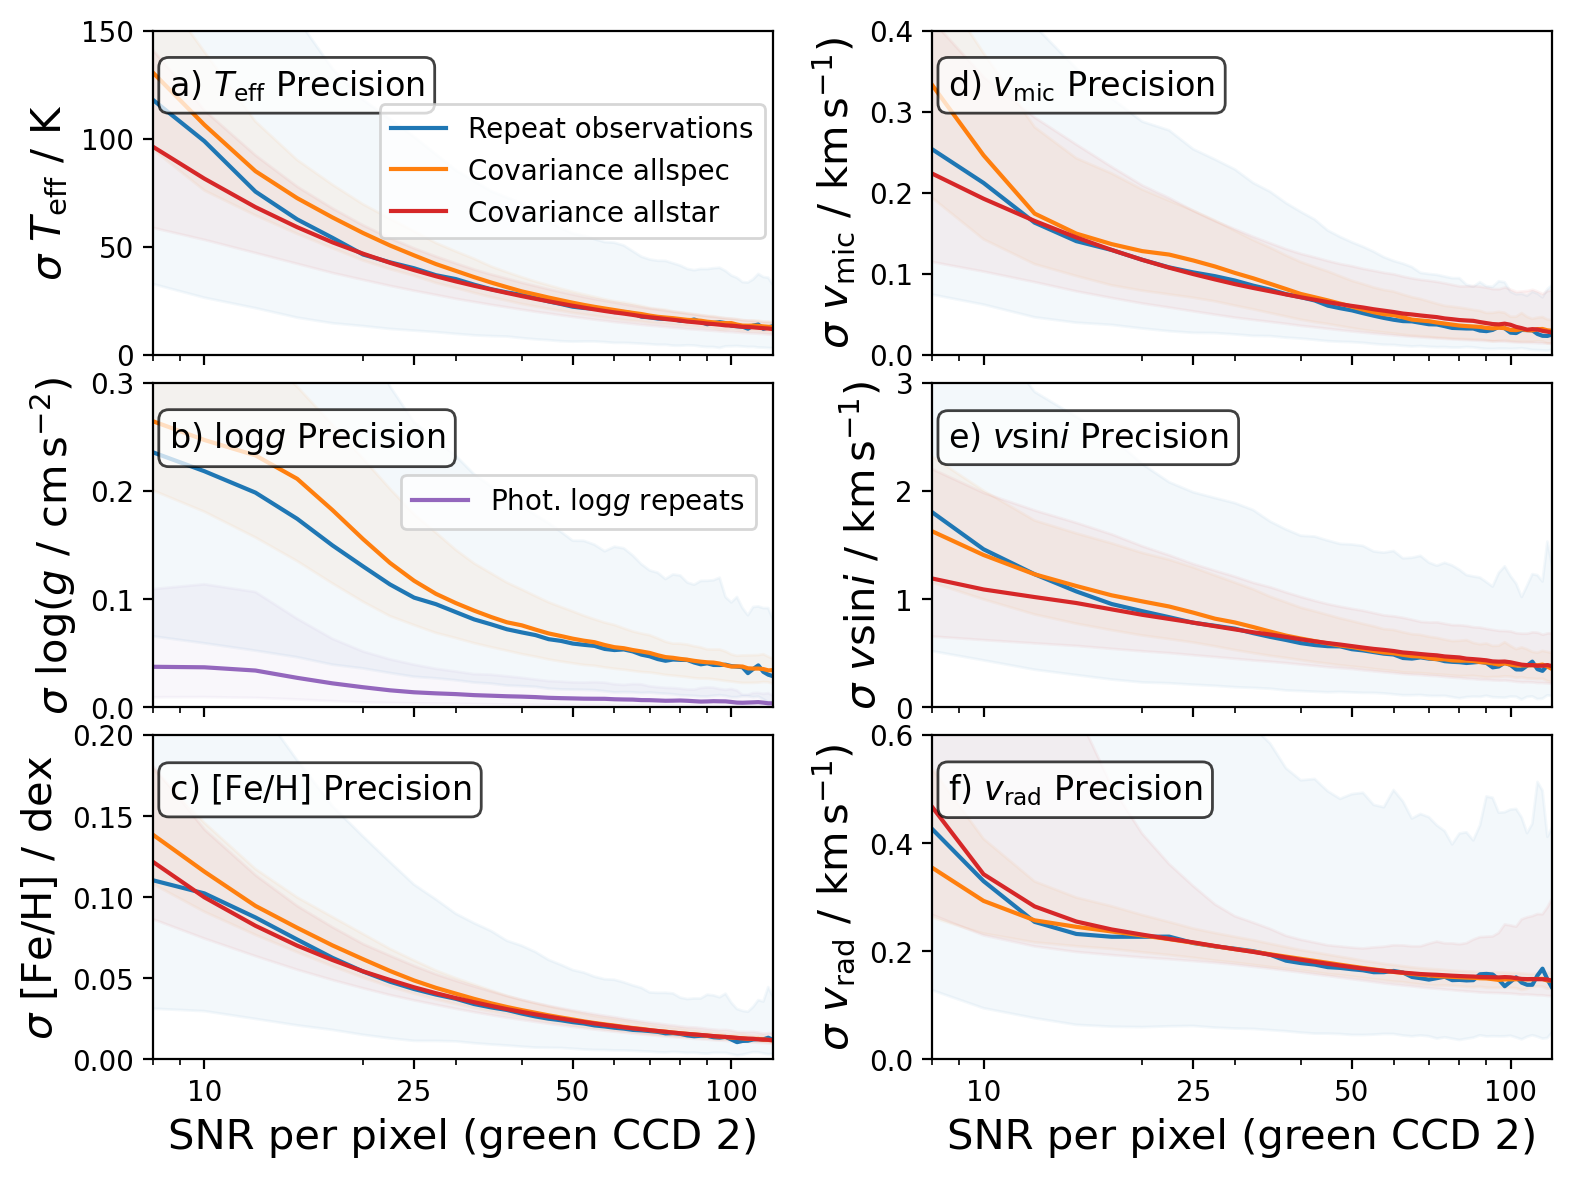
\includegraphics[width=\textwidth]{figures/galah_dr4_precision_parameters.png}
 \caption{\textbf{Precision monitoring of stellar parameters as a function of SNR for the green CCD2 across GALAH DR4.}. Each panel shows the behaviour for bins of width 10 for the scatter of repeat observations of the allspec runs (blue), covariance uncertainties of allspec (orange) and allstar (red) setups as well as scatter of photometric \logg from repeat observations (purple).}
 \label{fig:galah_dr4_precision_parameters}
\end{figure}

\begin{figure*}[ht]
 \centering
 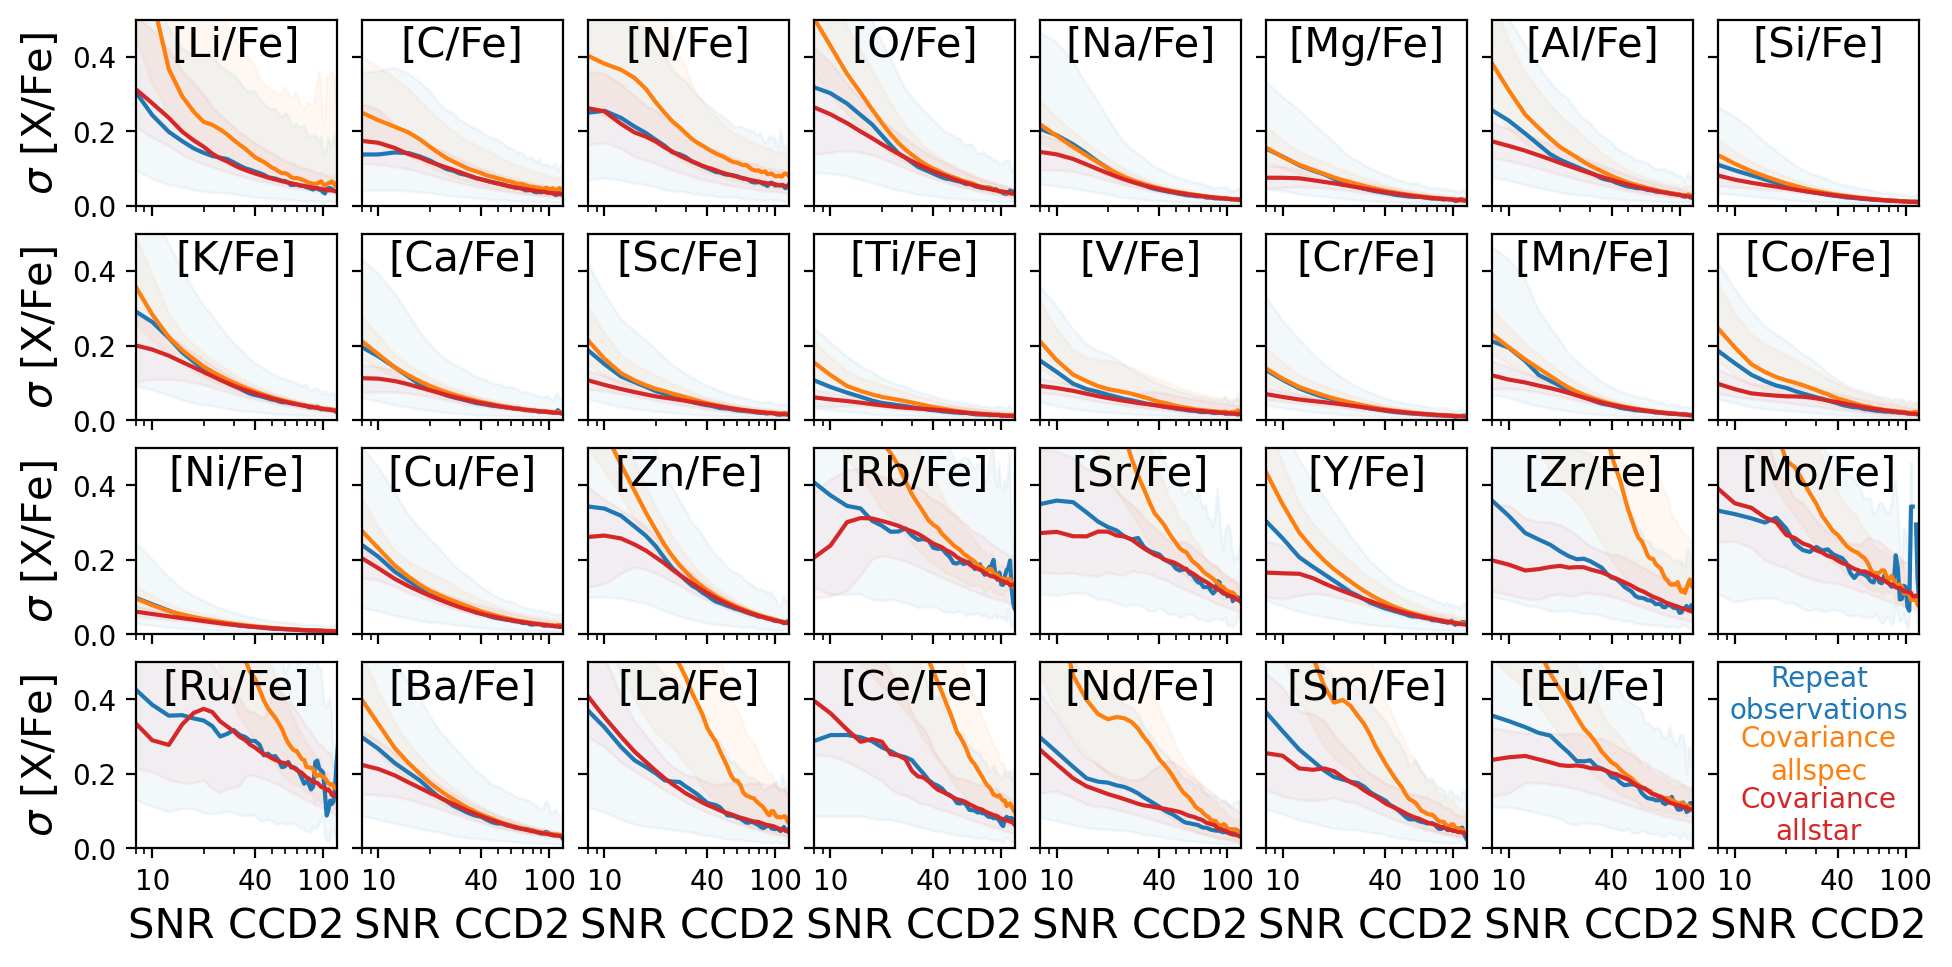
\includegraphics[width=\textwidth]{figures/galah_dr4_precision_abundances.png}
 \caption{\textbf{Precision monitoring of elemental abundances as a function of SNR for the green CCD2 across for GALAH DR4.}. Each panel shows the behavior for bins of width 10 for the scatter of repeat observations of the allspec runs (blue) as well as covariance uncertainties of allspec (orange) and allstar (red) setups. \SB{Missing legend}}
 \label{fig:galah_dr4_precision_abundances}
\end{figure*}

%        \item intrinsic scatter in clusters: M~67, 
%    \end{itemize}
%    \item 
%    \item Globular Clusters:
%    \begin{itemize}
%        \item 
%        \item NGC~104 / 47Tuc
%        \item NGC~288
%        \item NGC~362
%        \item Omega Cen: 
%        \item NGC~1851: \citet{Yong2015}, including CNO
%        \item NGC~6121 / M~4?
%        \item NGC~6362
%        \item NGC~6397
%        \item NGC~7099 / M~30
%        \item We have observed also NGC~4590 / M~68, NGC~5986, NGC~6144, NGC~6541, NGC~6584, NGC~6723, BH~140 and E~3.
%\end{itemize}
%    
%\end{itemize}

\SB{Giribaldi Titans [Fe/H] stars }

\subsubsection{Covariances} \label{sec:uncertainty_covariance}

We also calculate and report the covariances of all fitted labels, see Fig.~\ref{fig:covariance_vesta_arcturus} for Vesta and Arcturus.

\begin{figure*}[ht]
 \centering
 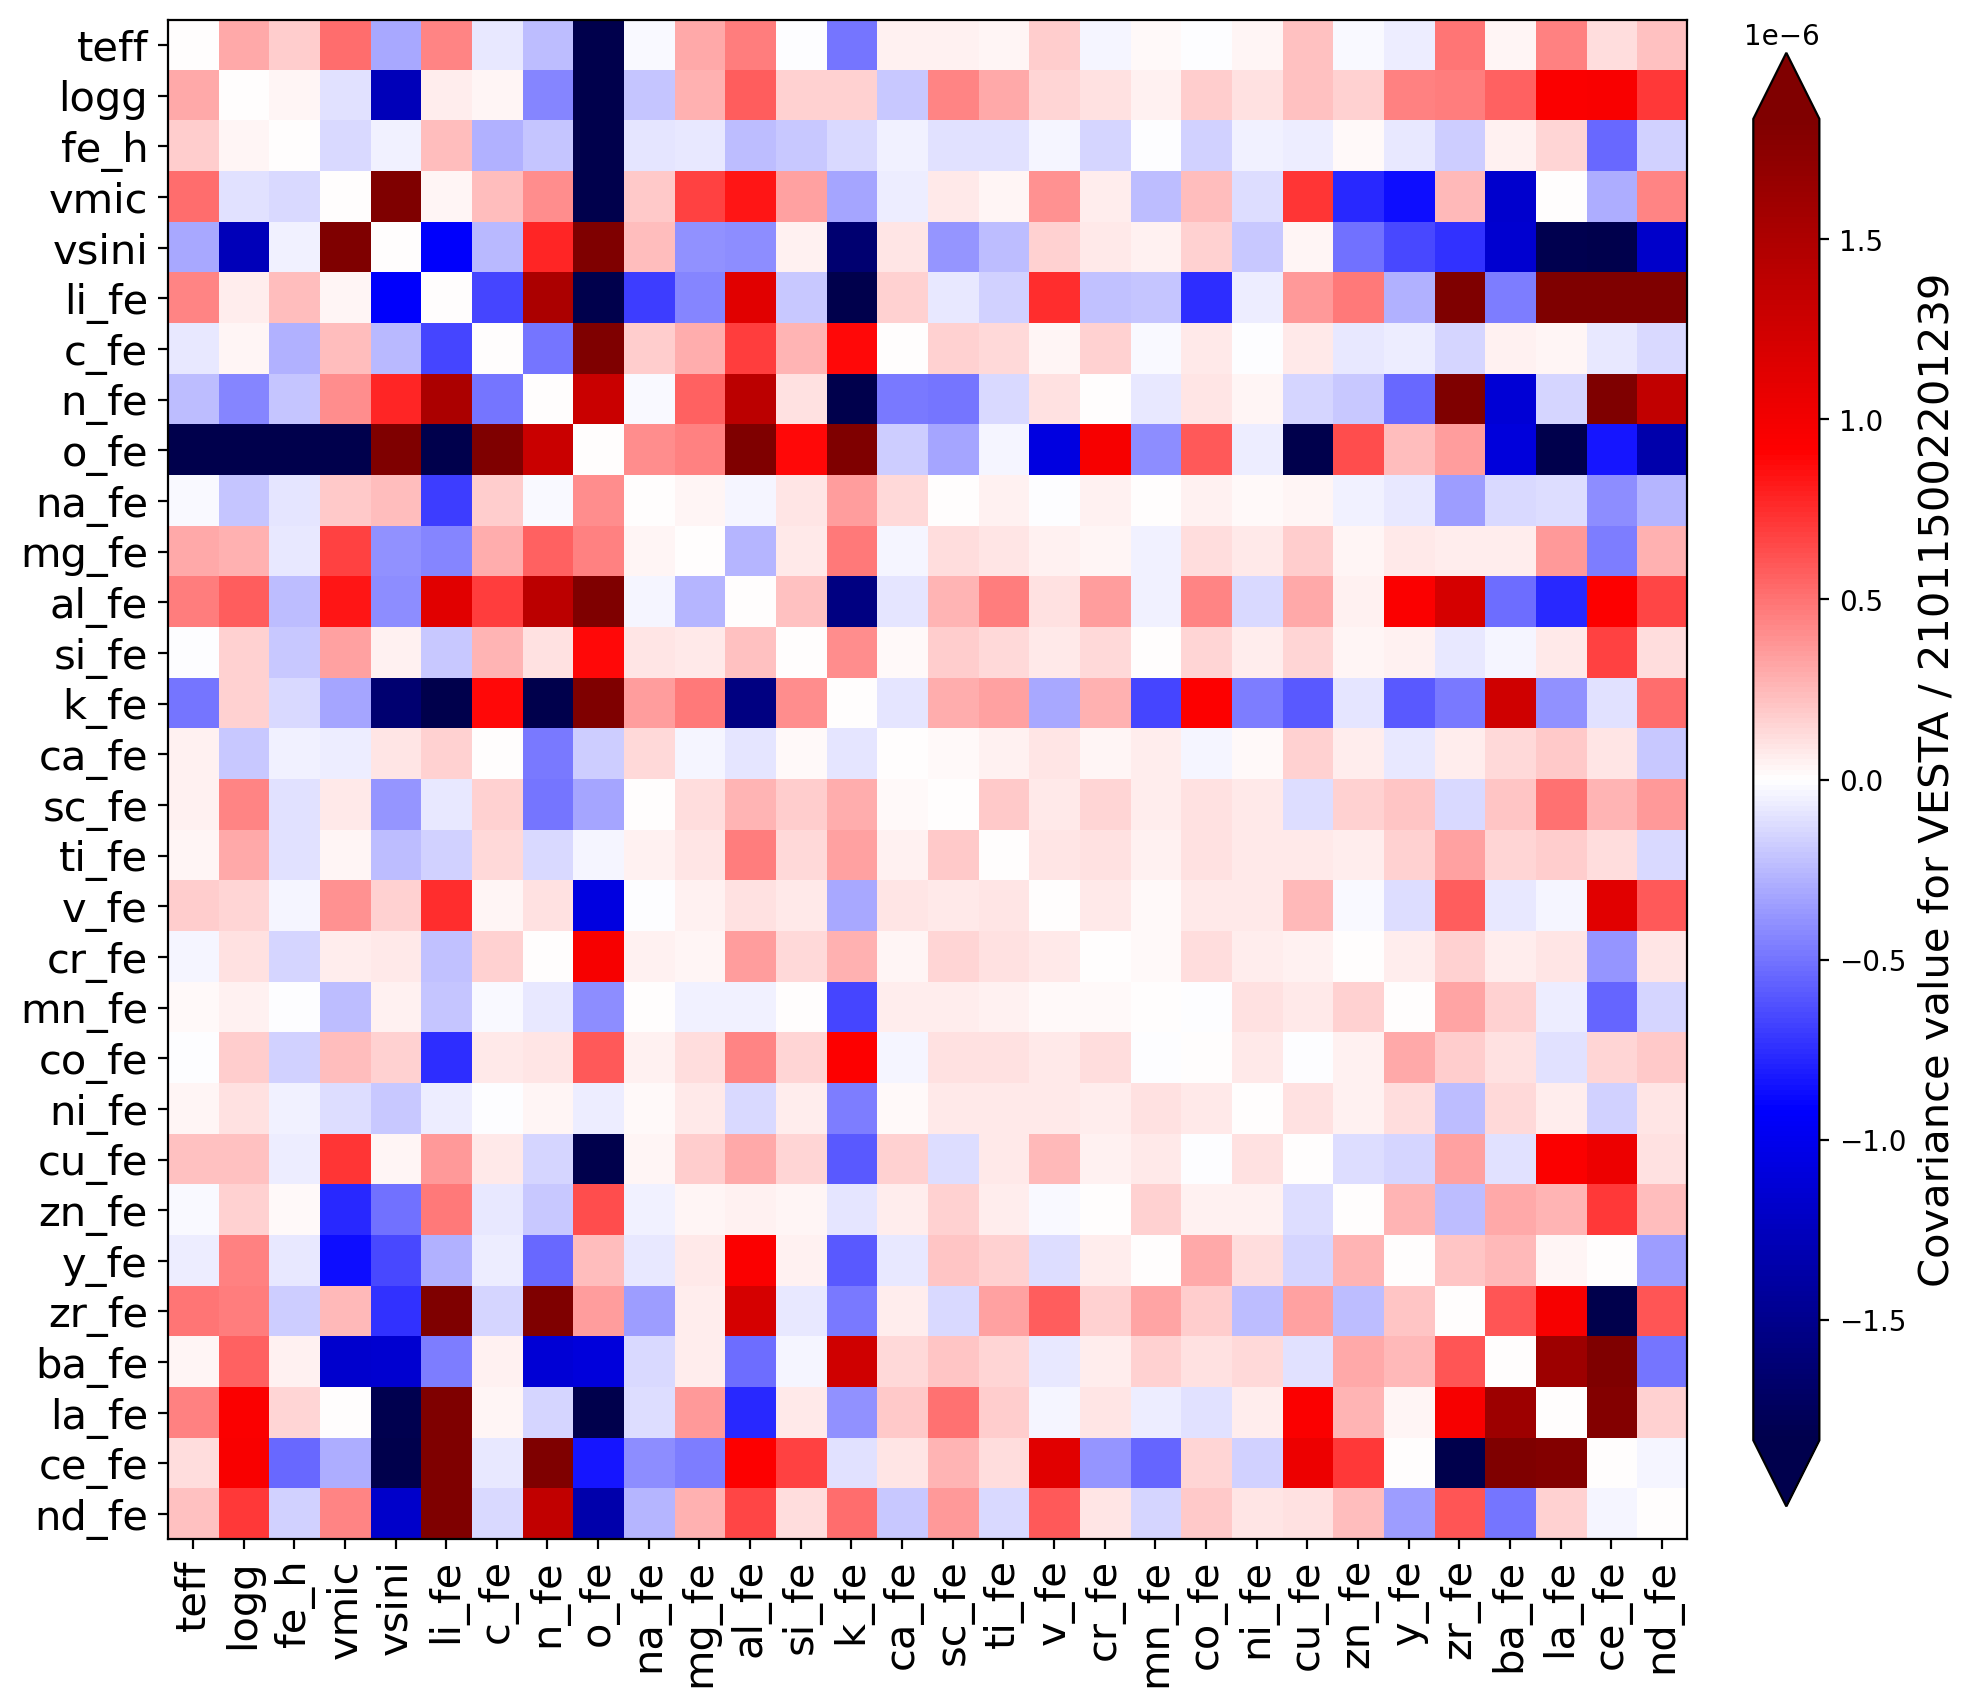
\includegraphics[width=0.49\textwidth]{figures/covariance_vesta.png}
 \hfill
 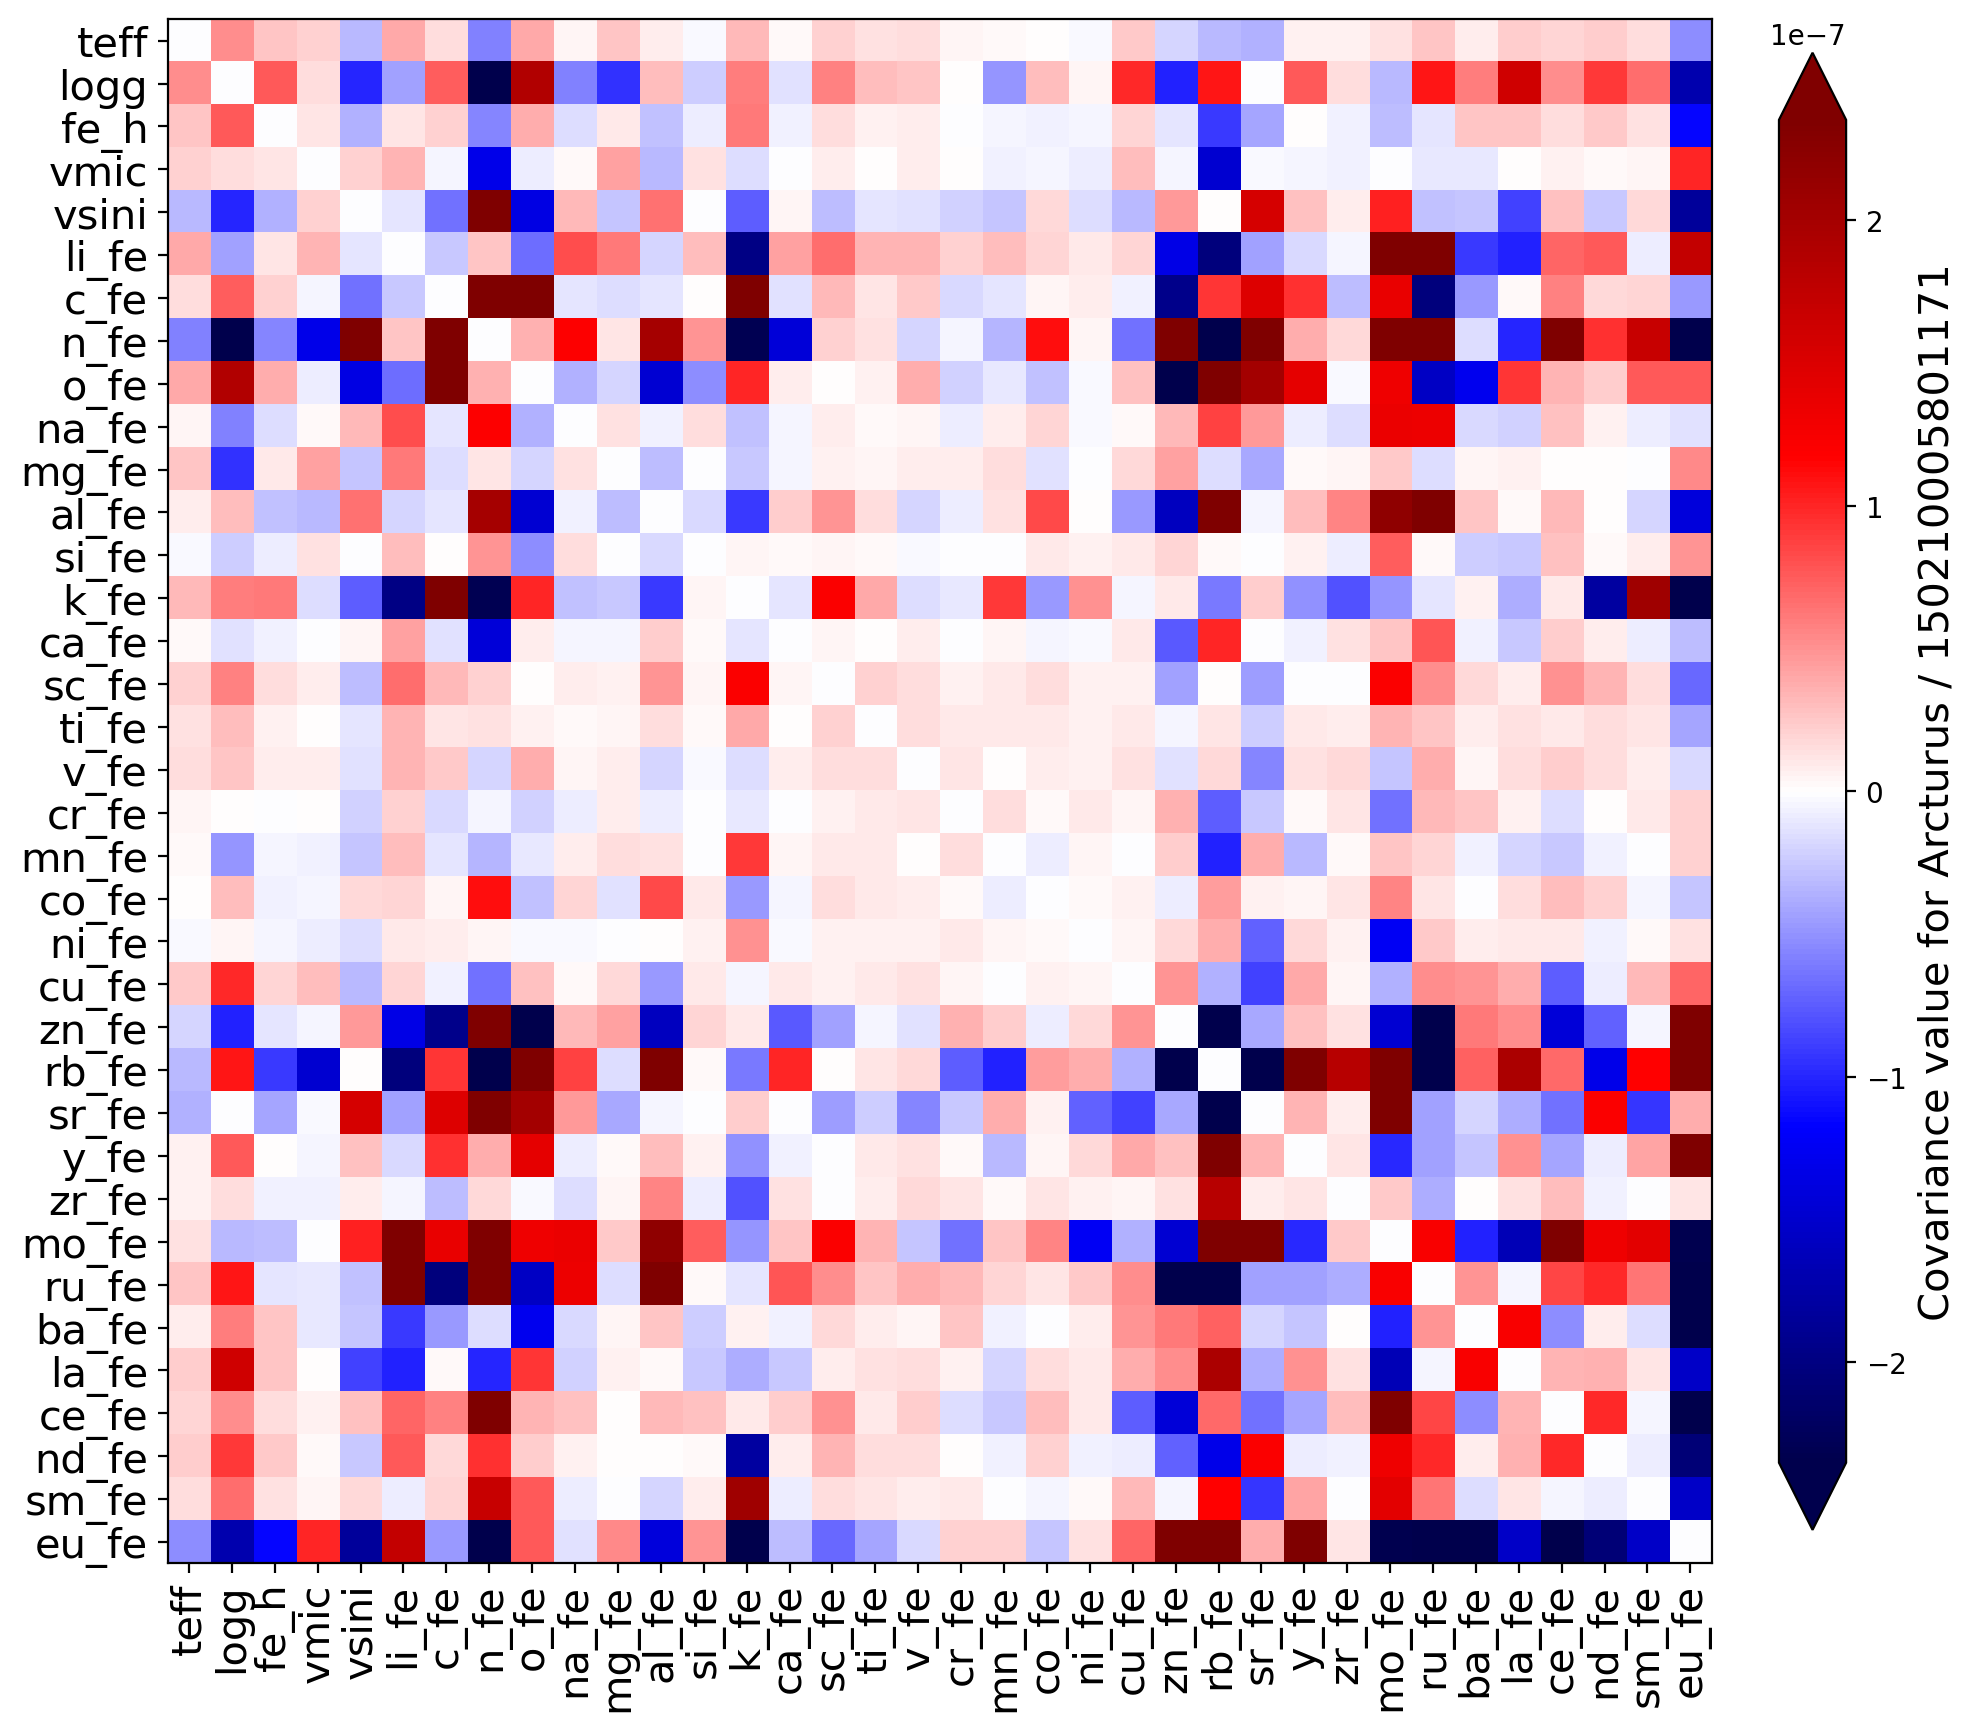
\includegraphics[width=0.49\textwidth]{figures/covariance_arcturus.png}
 \caption{\textbf{Covariance matrices for labels for Vesta (panel a) and Arcturus (panel b).}}
 \label{fig:covariance_vesta_arcturus}
\end{figure*}


%%%%%%%%%%%%%%%%%%%%%%%%%%%%%%%%%%%%%%%%%%%%%%%%%%%%%%%%%%%%%%%%%%%%%%%%%
\subsection{Stellar parameter flags \textsc{flag\_sp}}
\label{sec:flag_sp}
%%%%%%%%%%%%%%%%%%%%%%%%%%%%%%%%%%%%%%%%%%%%%%%%%%%%%%%%%%%%%%%%%%%%%%%%%

We have implemented a number of post-processing routines for quality assurance. Here, we describe the major quality flags of global parameters and overall fitting performance. If a spectrum does not pass one of these tests, a unique bit flag will be raised and added to \texttt{flag\_sp}.

The description of the implemented bits/flags for \texttt{flag\_sp} and how often they were raised is listed in Tab.~\ref{tab:flag_sp} and distributions in the Kiel diagram (\Teff and \logg) are shown for each raised bit in Fig.~\ref{fig:flag_sp_overview_allstar} for the \textit{allstar} catalogue.

\SB{Describe how the vsini and vmic flags are quite informative about binarity. Look at the binary main sequence for that!}

\SB{SB2 warning currently often activated for luminous RGB stars. Is that maybe caused by detectable extinction? Inspect more examples and figure out what is going on!}

\SB{Why are the chi2 stars mainly on the RGB? We use a strict cutoff value rather than an SNR dependent one. Maybe implement an SNR dependent on (GBS stars are also all flagged because of this issue)?}

Fig.~\ref{fig:examples_flag_sp_1} and Fig.~\ref{fig:examples_flag_sp_2}

In python, the check for a bitmask flag (e.g. 3rd flag with value $2^3 = 8$) is best performed via 
\begin{verbatim}
    flag_8_raised = (galah_dr4['flag_sp'] & 8) != 0
\end{verbatim}

\begin{table}[ht]
\centering
\caption{List of major quality flag \texttt{flag\_sp} listing the bit, description and how often the flag was raised for the \textit{allstar} and \textit{allspec} routines. Notes: Multiple bits can be raised for each of the 1\,085\,520 spectra spectra of the  of 917\,588 stars.}
\label{tab:flag_sp}
\begin{tabular}{ccccc}
\hline \hline
Raised Bit & Flag & Description & \textit{allstar} & \textit{allspec} \\
\hline
  & 0 & No flag & 700125 & 663075 \\ 
0 & 1 & Emission & 9568 & 7646 & \\
1 & 2 & CCD missing & 70078 & 44344 & \\
2 & 4 & Spectr. Binary 1 & 0 & 25538 & \\
3 & 8 & Spectr. Binary 2 & 34833 & 32566 & \\
4 & 16 & $\chi^2 > 3\sigma$ & 66859 & 20544 & \\
5 & 32 & \vsini warning & 138317 & 95990 & \\
6 & 64 & \vmic warning & 99692 & 78686 & \\
7 & 128 & Triple Binary warning & 0 & 0 & \\
8 & 256 & \Teff warning & 0 & 0 & \\
9 & 512 & \logg warning & 19863 & 10900 & \\
10 & 1024 & \feh warning & 0 & 0 & \\
11 & 2048 & S/N low & 123736 & 71154 & \\
12 & 4096 & Not converged & 32986 & 0 & \\
13 & 8192 & Model extrapolated & 69613 & 5953 & \\
14 & 16384 & No Results & 7400 & 10899 & \\
\hline
\end{tabular}
\end{table}


\begin{figure*}[ht]
 \centering
 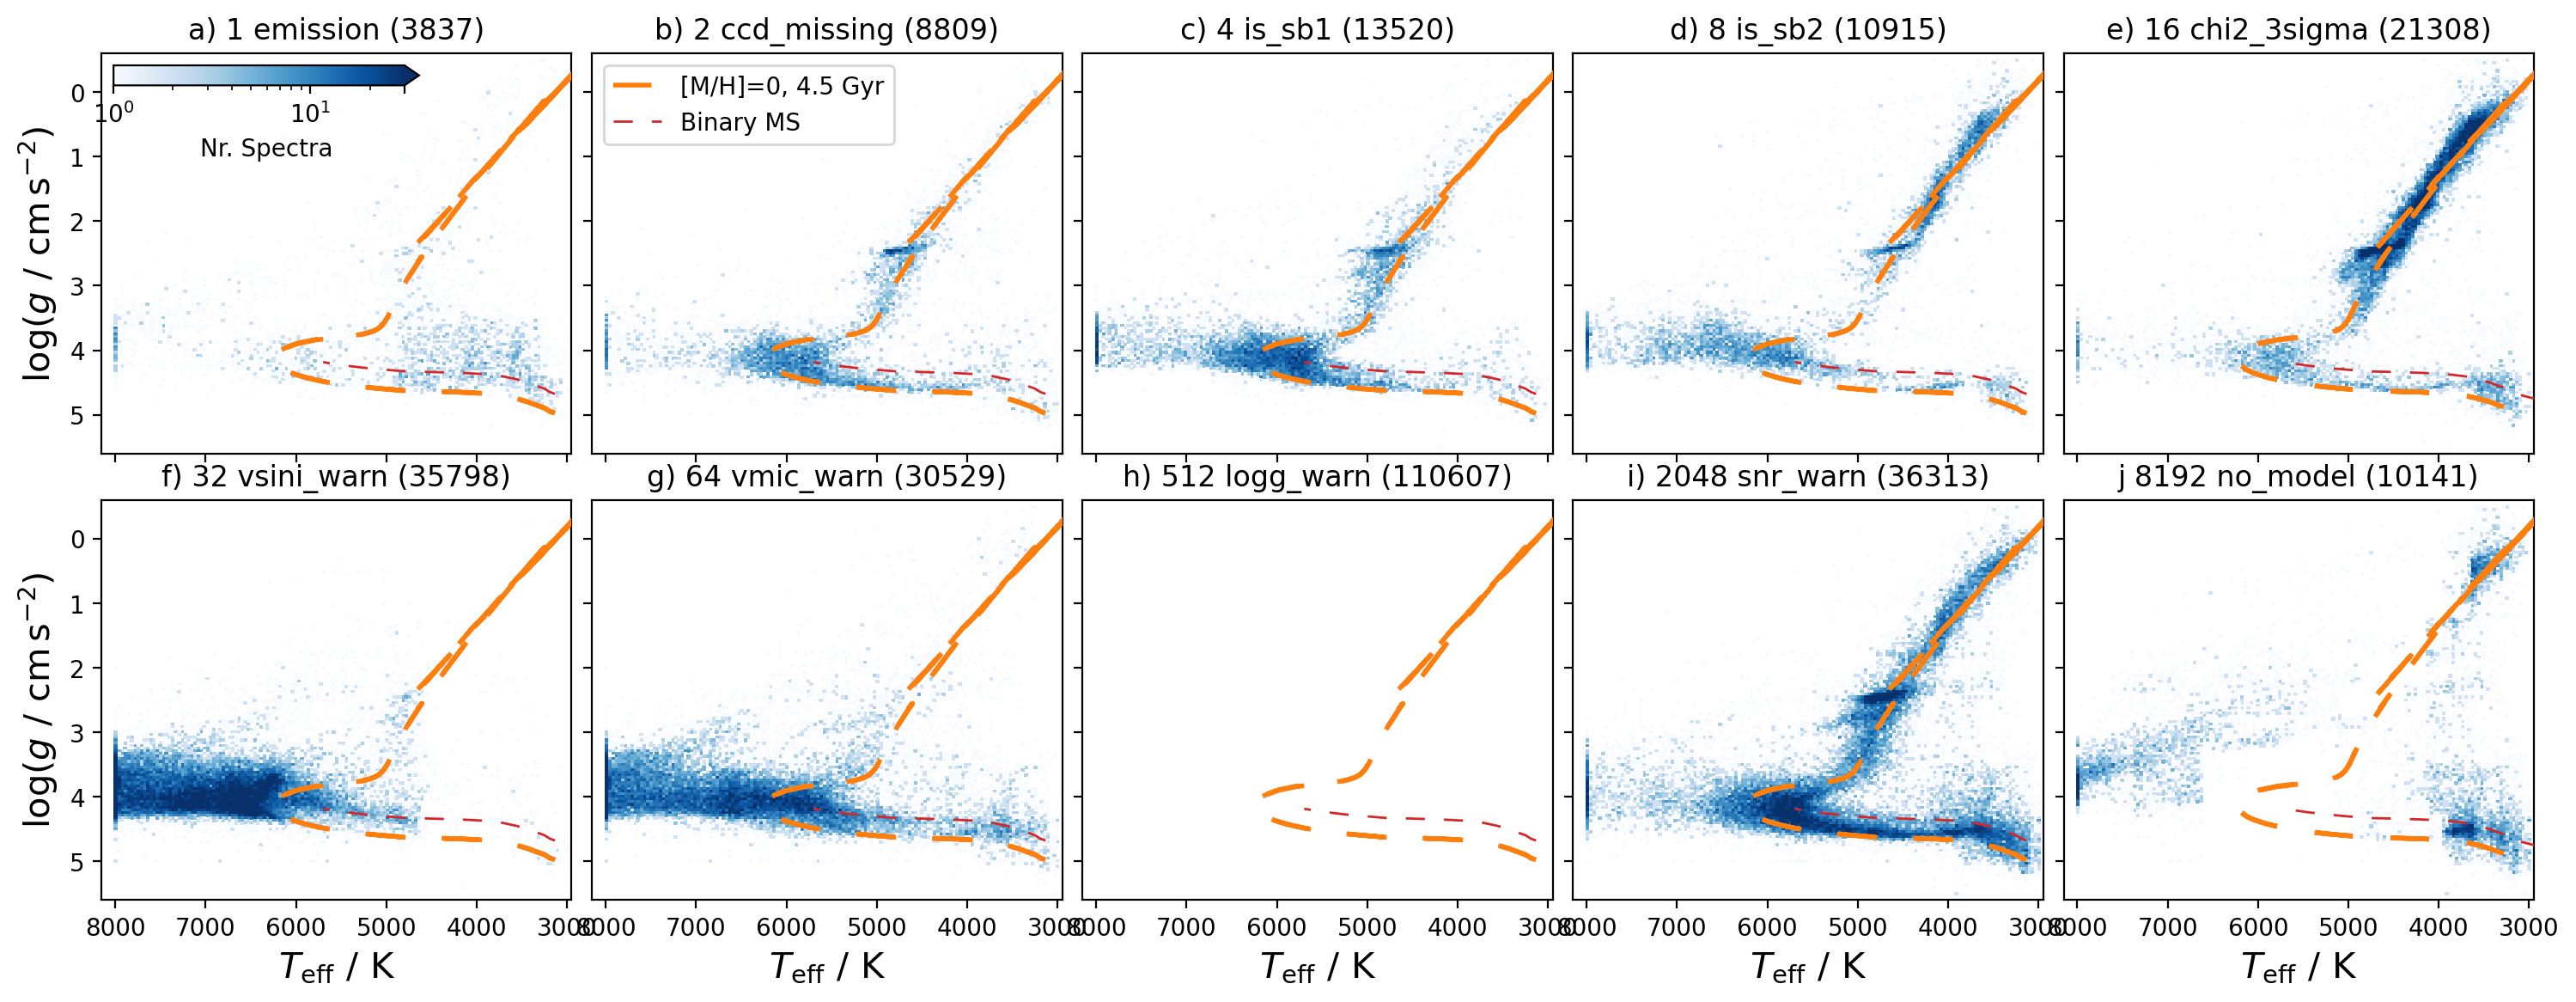
\includegraphics[width=\textwidth]{figures/flag_sp_overview_allstar.png}
 \caption{\textbf{Parameter overview of stars with raised major quality flag \texttt{flag\_sp} for \textit{allstar}.}
 \textbf{Each panel} shows the logarithmic density distribution of stars in the \Teff and \logg plane with blue colormaps. A PARSEC isochrone with $\mathrm{[M/H]}=0$ and $\tau = 4.5\,\mathrm{Gyr}$ is overplotted in orange and the same mass binary main sequence (shifted from the single star one by $\Delta \log g = -0.3\,\mathrm{dex}$) is shown in red. Panel heads denote the bit mask and its description as well as how many times the flag was raised. We neglect distributions with no flag (0), for flags which have not been raised (8,9,11), and for which no results were available (15).} \label{fig:flag_sp_overview_allstar}
\end{figure*}


%%%%%%%%%%%%%%%%%%%%%%%%%%%%%%%%%%%%%%%%%%%%%%%%%%%%%%%%%%%%%%%%%%%%%%%%%
\subsection{Elemental abundance flags \textsc{flag\_X\_fe}}
\label{sec:flag_x_fe}
%%%%%%%%%%%%%%%%%%%%%%%%%%%%%%%%%%%%%%%%%%%%%%%%%%%%%%%%%%%%%%%%%%%%%%%%%

\begin{table}
\centering
\caption{List of elemental abundance quality flags \texttt{flag\_fe\_h} for \feh or \texttt{flag\_X\_fe} for element X.}
\label{tab:flag_x_fe}
\begin{tabular}{ccc}
\hline \hline
Raised Bit & Flag & Description \\
\hline
  & 0 & detection \\ 
0 & 1 & upper limit \\ 
1 & 2 & no measurement available\\
2 & 4 & no convergence\\
3 & 8 & measurement above limit\\
4 & 16 & measurement below limit\\
5 & 32 & measurement issue of CNO \\
% problematic_cfe = (
%     # [C/N] < -1 for non-giants
%     (
%         (data['c_fe'] - data['n_fe'] < -1) & # [C/N] < -1
%         ~((data['logg'] < 3.5) & (data['teff'] < 5500)) # not_giant
%     ) |
%     # No [N/Fe] for non-giants
%     (
%         (data['flag_n_fe'] == 2) & # no [N/Fe]
%         ~((data['logg'] < 3.5) & (data['teff'] < 5500)) # not_giant
%     )
% )
%: $\mathrm{[C/N]} < -1$ for non-giants ($T_\text{eff} > 5500\,\mathrm{K}$ or $\log g > 3.5$) or no $\mathrm{[N/Fe]}$ measured for non-giants ($T_\text{eff} > 5500\,\mathrm{K}$ or $\log g > 3.5$) -> raising flag of $\mathrm{[C/Fe]}$ in that case as well as $\mathrm{[N/Fe]}$ extended non-giants ($T_\text{eff} > 5750\,\mathrm{K}$ or $\log g > 4.$ -> raising flag of $\mathrm{[N/Fe]}$ 
6 & 64 & measurement of Li, Ca, or Ba \\ %$ when CCD3 wavelength seems to be off (cdelt beyond the usual range of xx-xx) \\
\hline
\end{tabular}
\end{table}

%%%%%%%%%%%%%%%%%%%%%%%%%%%%%%%%%%%%%%%%%%%%%%%%%%%%%%%%%%%%%%%%%%%%%%%%%
\subsection{Abundance detection or upper limit}
\label{sec:abundance_detection_or_upper_limit}
%%%%%%%%%%%%%%%%%%%%%%%%%%%%%%%%%%%%%%%%%%%%%%%%%%%%%%%%%%%%%%%%%%%%%%%%%

To assess whether the abundance estimates are a true detection or an upper limit for element X, we produce synthetic spectra with the same stellar labels, but decrease the abundance [X/Fe] to the lower limit of the neural network (or decrease the \feh value by -0.5 for Fe). The residuals in units of sigma between the best-fit spectrum and spectrum with lowest possible [X/Fe] or lowered \feh then allow us to identify a detection (with maximum differences beyond 3 sigma) or upper limits, for which we raise the flag \textsc{flag\_x\_fe} by 1. We note that our initial test of overall detectability (Sec.~\ref{sec:which_labels_are_optimised}) allowed us identify elements for which not even an upper limit was expected, raising flag \textsc{flag\_x\_fe} by 2.

%Our pipeline will find the most suitable model and in particular set of abundances for the given observation. That does, however, not necessarily mean that the abundance of each element is actually well determined, because lines of the element may actually not be detected. For each element, we therefore run a post-processing routine to estimate if the measured abundance is indeed significant compared to the uncertainty of the spectrum. For each star, we therefore take the best-fit labels and neural network model and assess the change in the model spectrum when changing one abundance at a time to the lower boundary of the neural network model. If the difference between the spectrum of the best-fit and the lowest possible abundance is not above $3\sigma$ for a given elemental label, we do not consider it a reliable detection and thus raise the flag \textsc{flag\_x\_fe} for this label.

%
%%%%%%%%%%%%%%%%%%%%%%%%%%%%%%%%%%%%%%%%%%%%%%%%%%%%%%%%%%%%%%%%%%%%%%%%%%
%% \subsection{Goodness of fit}
%% \label{sec:goodness_of_fit}
%%%%%%%%%%%%%%%%%%%%%%%%%%%%%%%%%%%%%%%%%%%%%%%%%%%%%%%%%%%%%%%%%%%%%%%%%%
%
%% Raise flag\_sp by 4
%
%% \subsection{Rotational broadening}
%
%% vsini only provided from 1.5 to 24.
%
%% Values below 0 and above 25 raise flag\_sp b 8
%
%% \subsection{Emission lines}
%
%% We use the composite trapezoidal rule to estimate equivalent width for emission based on the difference between observed and model spectrum around $2\,\mathrm{\AA}$ of each Balmer line. We flag the spectrum (raising flag\_sp by 16), if the observed spectrum is without a doubt in emission with a median observed flux above zero for the Balmer line cores ($\pm 0.5\,\mathrm{\AA}$ of the line center).
%
%% \subsection{Flagging of problematic measurements}
%
%% \SB{Flag if parameters outside of the range of \TheCannon (e.g. \vsini$ > 30 \kms$, see Sec.~\ref{subsubsec:polynomials})}
%
%% \SB{Flag if parameters are outside of convex hull of isochrone grid, when using photoastrometric information. Also note that we have cut away \Teff above $10,000\K$ and \logg above $6\dex$.}


%%%%%%%%%%%%%%%%%%%%%%%%%%%%%%%%%%%%%%%%%%%%%%%%%%%%%%%%%%%%%%%%%%%%%%%%%
\section{VALIDATION}
\label{sec:validation}
%%%%%%%%%%%%%%%%%%%%%%%%%%%%%%%%%%%%%%%%%%%%%%%%%%%%%%%%%%%%%%%%%%%%%%%%%

TESS CVZ asteroseismic info \citep{Hon2022} and tables from Hon\_2022\_AJ\_164\_135.fits

\subsection{Automatic Post-Processing Performance}

In this section, we try to estimate how reliable the automatic flags in GALAH DR4 are.

Spectra have been classified by eye
% saved at GALAH_DR4/validation/spectrum_classification_by_eye.xlsx

\begin{itemize}
    \item Spectroscopic Binary Type 1 (SB1) classification, Fig.~\ref{fig:examples_flag_sp_2}
    \item Spectroscopic Binary Type 2 (SB2) classification, Fig.~\ref{fig:examples_flag_sp_3}
    \item Equivalent width estimates of three diffuse interstellar bands (5780.59, 5797.19, $6613.66\,\text{\AA}$) with central wavelengths identified by \citet{Vogrincic2023} as well as for interstellar K ($7698.9643\,\text{\AA}$), see Fig.~\ref{fig:example_dibs_06453479-0102137}
    \item Emission classification and measurement, Fig.~\ref{fig:examples_flag_sp_1}
    \item Upper Limit estimation
\end{itemize}

\subsection{Comparison with GALAH DR3 and APOGEE DR17}

Fig.~\ref{fig:comparison_dr4_dr3_apo17}

\begin{figure}
 \centering
 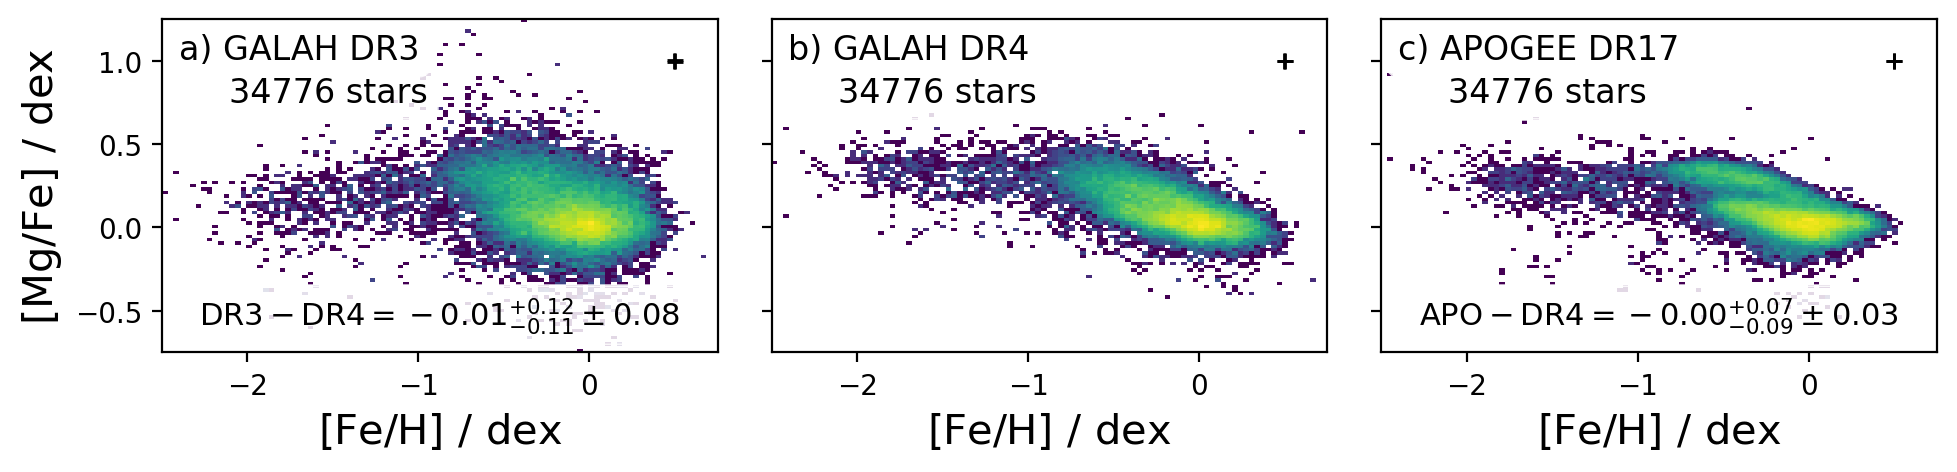
\includegraphics[width=\textwidth]{figures/comparison_dr4_dr3_apo17_Mg_fe.png}
 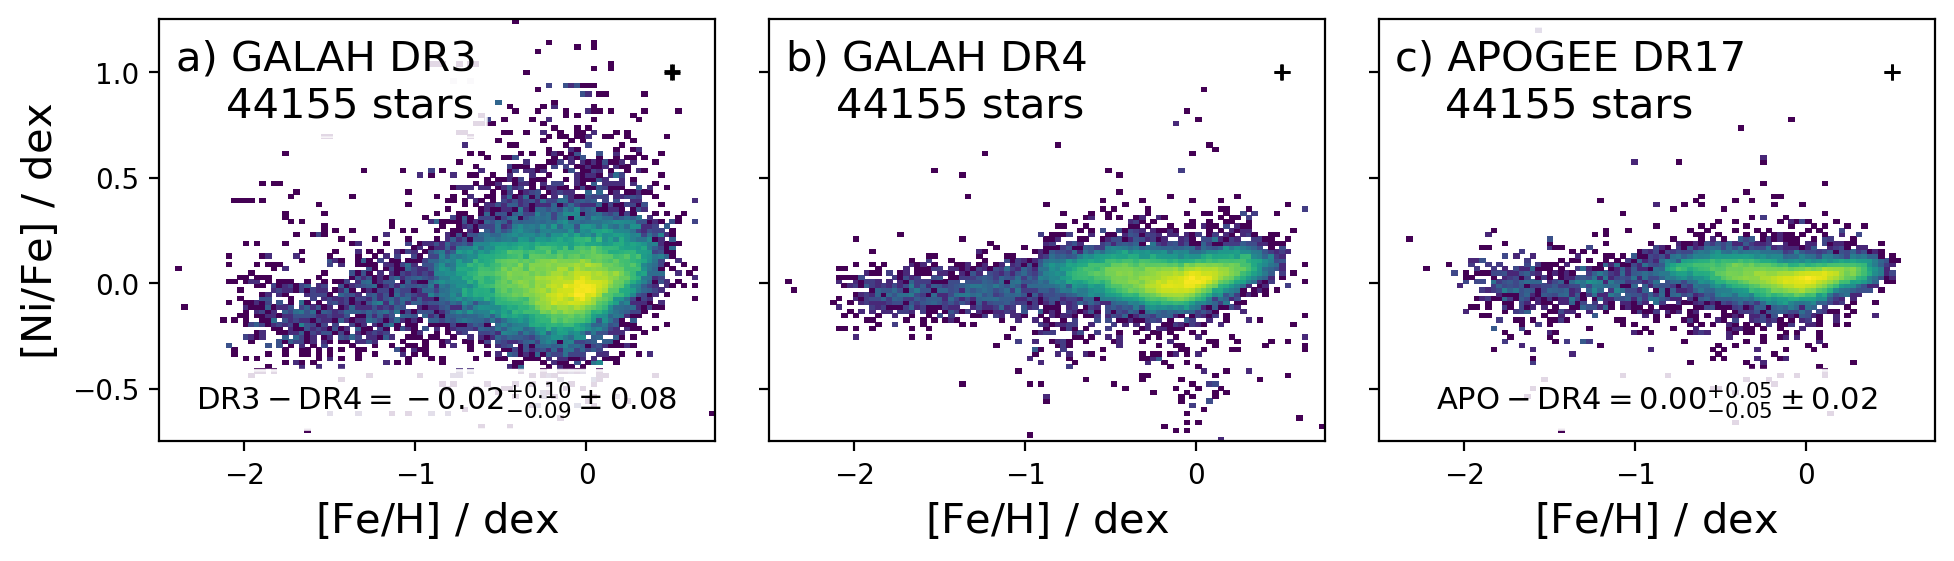
\includegraphics[width=\textwidth]{figures/comparison_dr4_dr3_apo17_Ni_fe.png}
 \caption{\textbf{Comparison of stars with measurements for all of GALAH DR3 (left panel), GALAH DR4 (middle panel) as well as APOGEE DR17 (right panel) for [Mg/Fe] (top row), [Ni/Fe] (middle row)}.}
 \label{fig:comparison_dr4_dr3_apo17}
\end{figure}

\subsection{False positive rates for spectroscopic binaries}

Binaries from Bashi et al. : 2304.00043 \citep{Bashi2023}

Thanks to the radial velocity estimates provided for bright stars from the \Gaia radial velocity spectrometer \citep{Katz2022}, we have radial velocity estimates for 94\% (774\,914) of the stars observed for GALAH DR4.

Fig.~\ref{fig:vrad_comparison_comp1_comp2_gaiadr3}

\begin{figure*}[hbt]
 \centering
 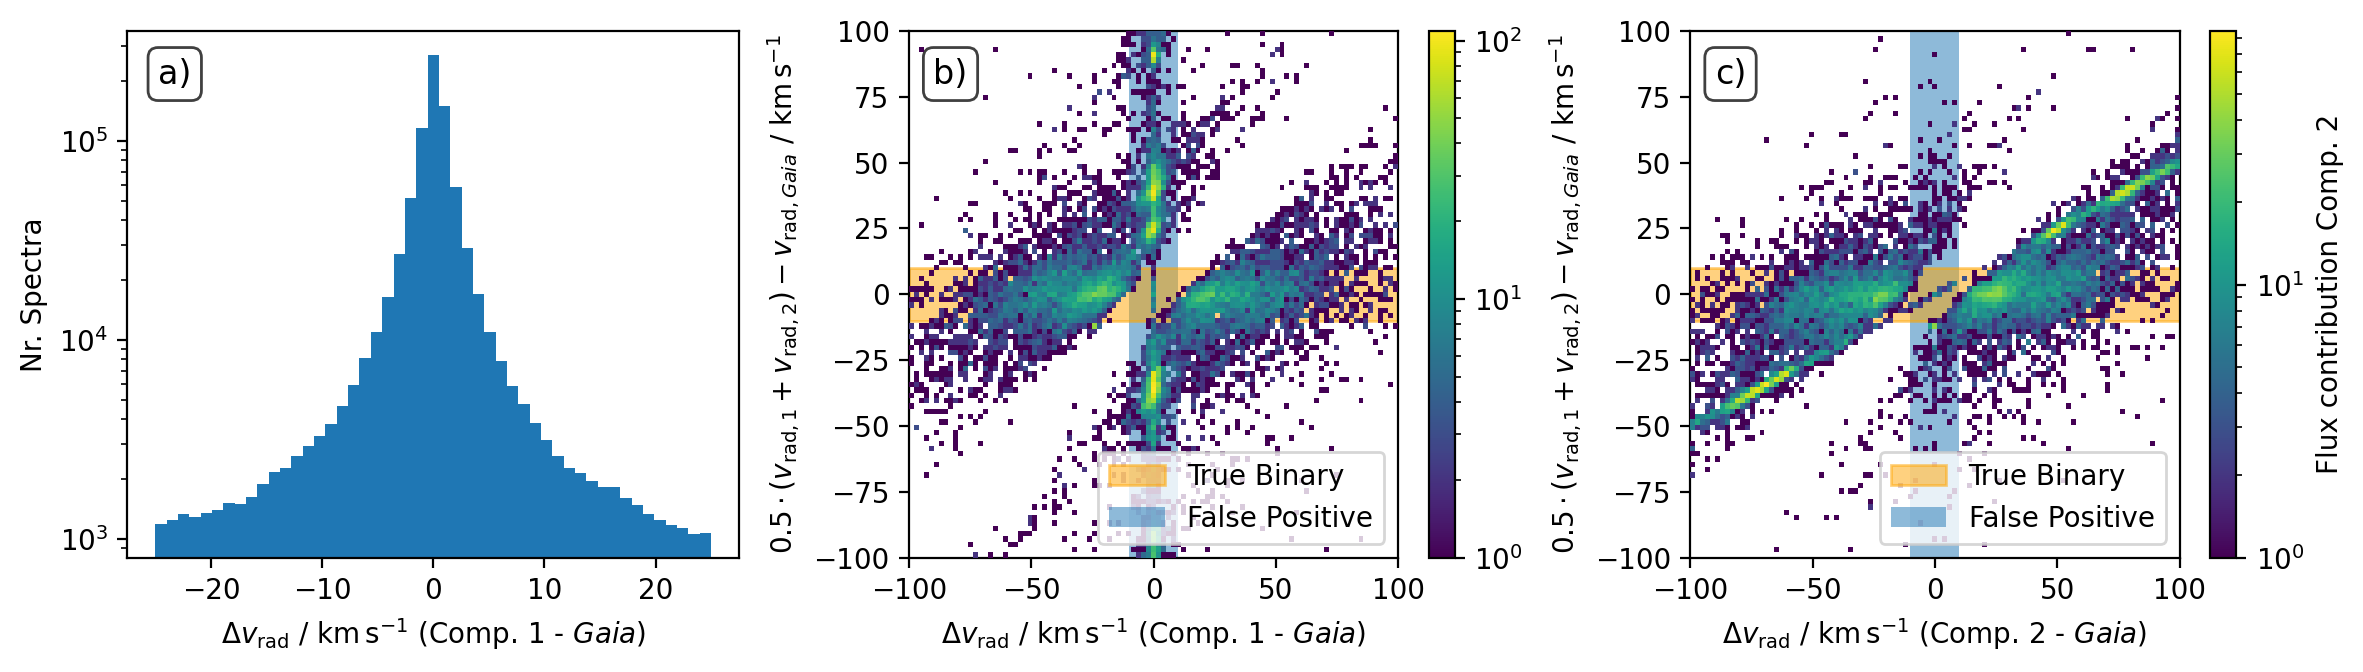
\includegraphics[width=\textwidth]{figures/vrad_comparison_comp1_comp2_gaiadr3.png}
 \caption{\textbf{Comparison of radial velocity estimates of GALAH DR4 and \textit{Gaia} DR3.} \textbf{Panel a)} shows the difference of GALAH's primary component radial velocity with the mean \textit{Gaia} DR3. \textbf{Panels b) and c)} show stars for which two components were detected in GALAH DR3 and shows the difference between each component and \textit{Gaia} DR3 against the difference of mean (roughly systemic) radial velocities. The panels also include regions where actual binaries and false positive detections are expected.}
 \label{fig:vrad_comparison_comp1_comp2_gaiadr3}
\end{figure*}

Binarity. How accurate is the flagging. Compare ratios of true/false, false-positive detections aided by \citet{Traven2020}. Get in contact with Alex Wallace and Andy Casey regarding their binarity identification from BP/RP spectra.

\subsection{Variable stars in GALAH DR4}

We have crossmatched the sources from GALAH DR4 with those from \Gaia DR3's variability catalogues \citep{Rimoldini2023}.

\begin{table}
\centering
\caption{\textbf{Overlap of GALAH DR4 with \textit{Gaia} DR3 variability catalogues.} Classifications are taken from the \textit{gaiadr3.vari\_classifier\_result} table and described in \cite{Rimoldini2023}. Abbreviations: ACV ({$\upalpha^2$}Canum Venaticorum), MCP and CP ((magnetic) chemically peculiar), ROAM and ROAP (rapidly oscillating Am- and Ap-type), SXARI (SXArietis), BE (B-type emission line), GCAS ({$\upgamma$}Cassiopeiae), SDOR (SDoradus), WR (Wolf-Rayet), DSCT ({$\updelta$}Scuti), GDOR ({$\upgamma$} Doradus), SXPHE (SXPhoenicis), SOLAR\_LIKE (solar-like variable, including BY Draconis type, rotating spotted star, and flaring stars).}
\label{tab:overlap_gaiadr3_vari}
\begin{tabular}{ccc}
\hline \hline
Classification & DR4 allspec & DR4 allstar \\
\hline
ACV \vert CP\vert MCP\vert ROAM\vert ROAP\vert SXARI & 330 & 285 \\
ACYG ({$\upalpha$}Cygni-type) & 45 & 34 \\
BCEP ($\upbeta$Cephei) & 16 & 15 \\
BE\vert GCAS\vert SDOR\vert WR & 67 & 54 \\
CEP (Cepheid) & 133 & 103 \\
CV (cataclysmic variable) & 3 & 3 \\
DSCT\vert GDOR\vert SXPHE & 16342 & 14477 \\
ECL (eclipsing binary) & 4610 & 4074 \\
ELL (ellipsoidal variable) & 95 & 11 \\
EP (star with exoplanet transits) & 19 & 14 \\
LPV (long-period variable) & 7351 & 6247 \\
RCB (R Coronae Borealis variable) & 4 & 1 \\
RR (RR Lyrae type) & 561 & 401 \\
RS (RS Canum Venaticorum variable) & 3950 & 3355 \\
S (short-timescale object) & 40 & 33 \\
SDB (subdwarf B star) & 6 & 6 \\
SOLAR\_LIKE & 20027 & 17256 \\
SPB (slowly pulsating B-type variable) & 31 & 24 \\
SYST (symbiotic variable star) & 3 & 3 \\
WD (variable white dwarf) & 1 & 1 \\
YSO (young stellar object) & 1534 & 1096 \\
\hline
Total & 55168 & 47493 \\
\hline
\end{tabular}
\end{table}

\SB{Put list of vari catalogues and their respective publications in here, e.g. \Gaia DR3 binary star parameters from \texttt{gaiadr3.nss\_non\_linear\_spectro.fits} \citep{Halbwachs2023}.
}

1 White dwarf crossmatched, indeed the one (2MASS J05005185-0930549) that was found in GALAH data by \citet{Kawka2020}.

\subsection{Minimal Science Verification}

Fig. 3 from https://arxiv.org/abs/2203.05463: logAge vs. [C/N]

%%%%%%%%%%%%%%%%%%%%%%%%%%%%%%%%%%%%%%%%%%%%%%%%%%%%%%%%%%%%%%%%%%%%%%%%%
\section{DATA RELEASE PRODUCTS}
\label{sec:catalogues_release_products}
%%%%%%%%%%%%%%%%%%%%%%%%%%%%%%%%%%%%%%%%%%%%%%%%%%%%%%%%%%%%%%%%%%%%%%%%%

\subsection{Data release catalogues}
\label{sec:data_release_catalogues}

\begin{enumerate}
   \item galah\_dr4\_allspec.fits: analysis for each spectrum (incl. RV) assuming single star
   \item galah\_dr4\_allstar.fits: analysis for each star based on co-added spectra for each star and using non-spectroscopic information to constrain \logg
   \item galah\_dr4\_binary.fits: analysis for those spectra that are suspected line-splitting spectroscopic binaries (SB2) assuming two sources for spectrum with same \feh but different RV
\end{enumerate}

\begin{table*}
\caption{Table schema of the GALAH DR4 main catalogues.} \label{tab:main_catalog_schema1}
\centering
\begin{tabular}{lccc}
\hline\hline
Keyword	&	Type	&	Description	&	Section	\\
\hline
sobject\_id	&	int64	&	GALAH identifier	&		\\
tmass\_id	&	str	&	2MASS identifier	&		\\
gaiadr3\_source\_id	&	int64	&	Gaia DR3 source\_id	&		\\
survey\_name	&	str	&	HERMES-2dF Survey/Program/Pointing (other if not available)	&		\\
field\_id	&	int32	&	GALAH Field ID (-1 if not available)	&		\\
setup	&	str	&	Analysis setup: single/binary/coadds	&		\\
mjd	&	float32	&	Modified Julian Date	&		\\
ra	&	float64	&	propagated from Gaia DR3	&		\\
dec	&	float64	&	propagated from Gaia DR3	&		\\
best\_spec4star	&	bool	&	Best spectrum for given star (identifiable via 2MASS ID)	&		\\
flag\_sp	&	int32	&	Major spectroscopic quality bitmask flag	&		\\
flag\_sp\_fit	&	int32	&	Major spectroscopic fitting quality bitmask flag	&		\\
opt\_loop	&	int32	&	Nr of optimisation loops used for fitting	&		\\
flag\_red	&	int32	&	Quality bitmask flag of reduction pipeline	&		\\
snr\_px\_ccdx	&	float32	&	Average signal-to-noise ratio (per pixel) of CCDX	&		\\
chi2\_sp	&	float32	&	Chi2 value of spectroscopic fitting	&		\\
px\_used\_perc	&	int64	&	Percentage of spectrum used for spectroscopic fit	&		\\
model\_name	&	str	&	Neural network model used for creating synthetic spectra	&		\\
closest\_model	&	str	&	Neural network model closest for \Teff/\logg/\feh combination	&		\\
comp\_time	&	float32	&	Computation time spent on spectrum	&		\\
flux\_contr	&	float32	&	Flux contribution of main source	&		\\
e\_flux\_contr	&	float32	&	Uncertainty flux\_contr	&		\\
rv\_comp\_nr	&	int64	&	Number of peaks in RV cross-correlation function (CCF)	&		\\
rv\_comp\_x	&	float32	&	Radial velocity of primary or secondary sourcex	&		\\
e\_rv\_comp\_x	&	float32	&	Uncertainty of rv\_comp\_x	&		\\
rv\_comp\_x\_h	&	float32	&	Height of rv\_comp\_x in CCF	&		\\
rv\_comp\_x\_p	&	float32	&	Prominence of rv\_comp\_x in CCF	&		\\
rv\_gaia\_dr3	&	float32	&	Radial velocity in Gaia DR3	&		\\
e\_rv\_gaia\_dr3	&	float32	&	Uncertainty of rv\_gaia\_dr3	&		\\
v\_bary\_eff	&	float64	&	Barycentric velocity applied to reduced spectra	&		\\
teff	&	float32	&	Spectroscopic effective temperature (used for fitting)	&		\\
e\_teff	&	float32	&	Uncertainty teff	&		\\
logg	&	float64	&	Surface gravity adjusted via parallax information	&		\\
e\_logg	&	float32	&	Uncertainty logg\_plx	&		\\
fe\_h	&	float32	&	Abundance of Fe and all other elements not fitted in GALAH (Fe: 1D-NLTE)	&		\\
e\_fe\_h	&	float32	&	Uncertainty fe\_h	&		\\
flag\_fe\_h	&	int32	&	Quality flag fe\_h	&		\\
vmic	&	float32	&	Microturbulence velocity (fitted)	&		\\
e\_vmic	&	float32	&	Uncertainty vmic	&		\\
vsini	&	float32	&	Broadening velocity (fitted sme.vsini with sme.vmac=0)	&		\\
e\_vsini	&	float32	&	Uncertainty of vsini	&		\\
x\_comp\_2	&	float32	&	Parameter value x of potential secondary source	&		\\
e\_x\_comp\_2	&	float32	&	Uncertainty of x\_comp\_2	&		\\
x\_fe	&	float32	&	Elemental abundance for [X/Fe]	&		\\
e\_x\_fe	&	float32	&	Uncertainty x\_fe	&		\\
flag\_x\_fe	&	int32	&	Quality bitmask flag of x\_fe	&		\\
\hline
\end{tabular}
\end{table*}

% \begin{table*}
% \caption{Table schema of the GALAH DR4 main catalogues. (Continuation of Tab.~\ref{tab:main_catalog_schema1}).} \label{tab:main_catalog_schema2}
% \centering
% \begin{tabular}{lccc}
% \hline
% Keyword	&	Type	&	Description	&	Section	\\
% \hline
% sb2\_rv\_16	&	float32	&	16th perc. radial velocity of fit to syn-obs residuals	&		\\
% sb2\_rv\_50	&	float32	&	50th perc. radial velocity of fit to syn-obs residuals	&		\\
% sb2\_rv\_84	&	float32	&	84th perc. radial velocity of fit to syn-obs residuals	&		\\
% ew\_h\_beta	&	float32	&	Equivalent Width of fit for syn-obs residuals at Hbeta core	&		\\
% ew\_h\_alpha	&	float32	&	Equivalent Width of fit for syn-obs residuals at Halpha core	&		\\
% ew\_k\_is	&	float32	&	Equivalent Width of fit for K7699 Interstellar Line	&		\\
% sigma\_k\_is	&	float32	&	Sigma auf Gaussian fit for K7699 Interstellar Line	&		\\
% rv\_k\_is	&	float32	&	Radial velocity of fit to syn-obs residuals around K7699 line	&		\\
% ew\_dibX	&	float32	&	Equivalent Width of fit for X Diffiuse Interstellar Band	&		\\
% sigma\_dibX	&	float32	&	Sigma auf Gaussian fit for X DIB	&		\\
% rv\_dibX	&	float32	&	Radial velocity of fit to syn-obs residuals around X DIB	&		\\
% logg\_spec	&	float32	&	Spectroscopic surface gravity (used for fitting)	&		\\
% e\_logg\_spec	&	float32	&	Uncertainty logg\_spec	&		\\
% phot\_g\_mean\_mag	&	float32	&	Mean Gaia DR3 G-band apparent magnitude	&		\\
% phot\_bp\_mean\_mag	&	float32	&	Mean Gaia DR3 BP-band apparent magnitude	&		\\
% bp\_rp	&	float32	&	Color of BP-RP bands	&		\\
% h\_m	&	float32	&	2MASS H-band magnitude	&		\\
% h\_msigcom	&	float32	&	Uncertainty of h\_m	&		\\
% ks\_m	&	float32	&	2MASS Ks-band magnitude	&		\\
% ks\_msigcom	&	float32	&	Uncertainty of ks\_m	&		\\
% W2mag	&	float32	&	AllWISE W2-band magnitude	&		\\
% e\_W2mag	&	float32	&	uncertainty of W2mag	&		\\
% ebv	&	float32	&	Extinction E(B-V)	&		\\
% parallax	&	float32	&	Astrometric parallax used for GALAH DR4	&		\\
% e\_parallax	&	float32	&	Uncertainty of astrometric parallax used for GALAH DR4	&		\\
% parallax\_gaia\_edr3	&	float32	&	Parallax reported with corrections by Gaia EDR3	&		\\
% e\_parallax\_gaia\_edr3	&	float32	&	Uncertainty of parallax reported with corrections by Gaia EDR3	&		\\
% ruwe\_gaia\_dr3	&	float32	&	RUWE reported by Gaia DR3	&		\\
% r\_med	&	float32	&	Median Distance used for calculating logg(plx)	&		\\
% r\_lo	&	float32	&	Lower Limit Distance used for calculating logg(plx)	&		\\
% r\_hi	&	float32	&	Higher Limit Distance used for calculating logg(plx)	&		\\
% a\_ks	&	float32	&	Attenuation in Ks-band A(Ks) used for calculating logg(plx)	&		\\
% mass	&	float32	&	Mass used for calculating logg(plx)	&		\\
% age	&	float32	&	Age estimated when calculating mass	&		\\
% bc\_ks	&	float32	&	Bolometric Correction of Ks, BC(Ks), used for calculating logg(plx)	&		\\
% lbol	&	float32	&	Bolometric Luminosity used for calculating logg(plx)	&		\\
% \hline
% \end{tabular}
% \end{table*}

\begin{landscape}
\begin{figure}
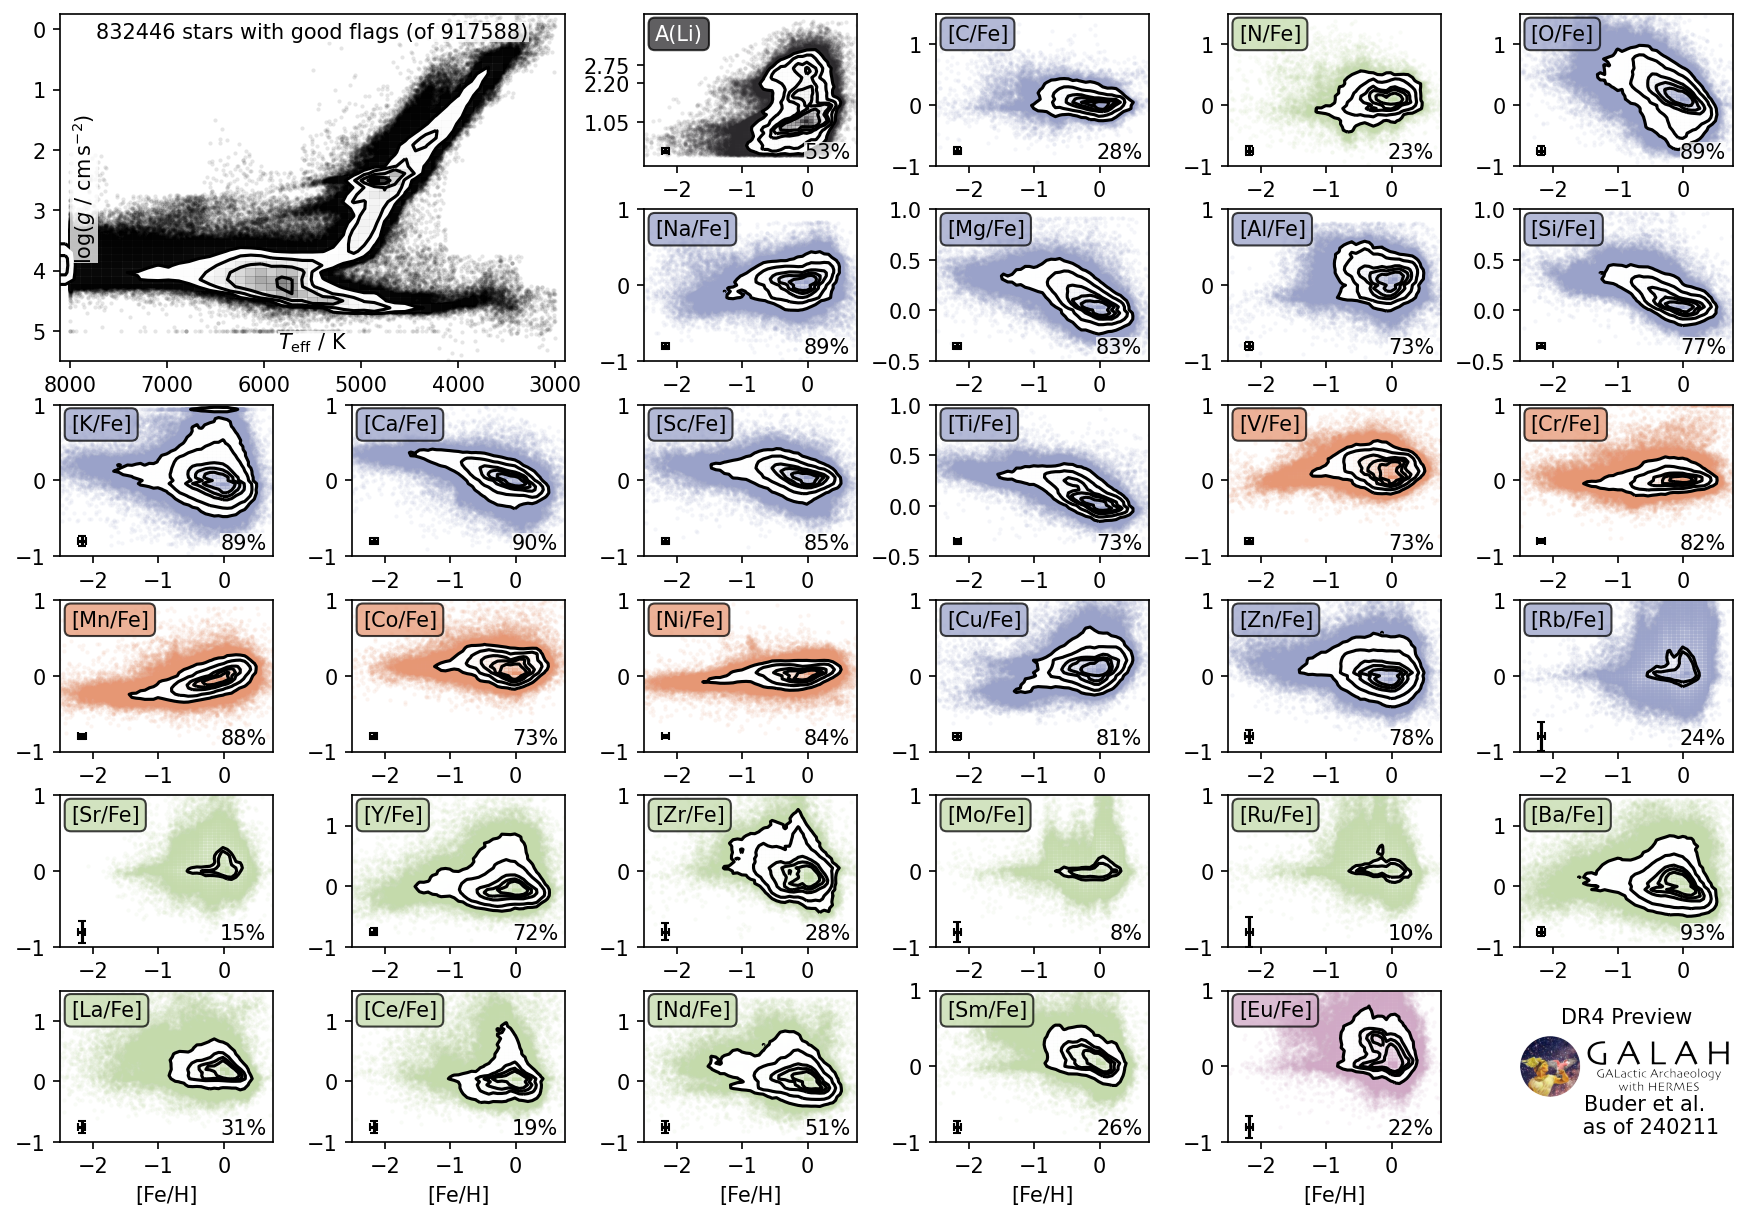
\includegraphics[width=0.975\columnwidth]{figures/galah_dr4_overview_allstar.png}
\caption{
\textbf{Overview of stellar parameters and elemental abundances for the \textit{allstar} estimates of GALAH DR4.}
\textbf{The top left panel} shows the density distribution of stars in the Kiel diagram of \Teff and \logg.
\textbf{All other panels} show the logarithmic elemental abundances (for elements indicated in the top left of the panel) as a function of the logarithmic iron abundances \feh. Elements are colored by different nucleosynthetic channels (black for big bang nucleosynthesis, blue for core-collapse supernovae, red for supernovae type Ia, green for asymptotic giant branch star contributions and pink for the rapid neutron capture process with contributions from merging neutron stars) following the color schema from \citet{Kobayashi2020}.
}
\label{fig:galah_dr4_overview_allstar}
\end{figure}
\end{landscape}


\subsection{Data products for each spectrum}
\label{sec:data_products_for_each_spectrum}

\begin{enumerate}
   \item 210115002201239\_single\_fit\_comparison.pdf (see Fig.~\ref{fig:210115002201239_single_fit_comparison}) \SB{Maybe actually use OmegaCen star 140314005201392: cool, metal-poor, strong CNO features and a good spectrum to explain why continuum points may not always work for a pipeline.}
   \item 210115002201239\_single\_fit\_covariances.npz
   \item 210115002201239\_single\_fit\_results.fits
   \item 210115002201239\_single\_fit\_rv.png (see Fig.~\ref{fig:181221003101356_single_fit_rv})
   \item 210115002201239\_single\_fit\_spectrum.fits
\end{enumerate}

For easier downloading, we also provide these files in tar-files per night. Furthermore, we have interpolated all normalised allstar spectra onto a common wavelength that includes the largest possible wavelength coverage of 99.9\% of radial velocity corrected spectra (neglecting pixels below 7680\AA for the infrared channel).

\subsection{Value-Added Catalogs}

\subsubsection{Dynamics}

Fig.~\ref{fig:galah_dr4_lz_jr_with_gcs}

\begin{landscape}
\begin{figure}
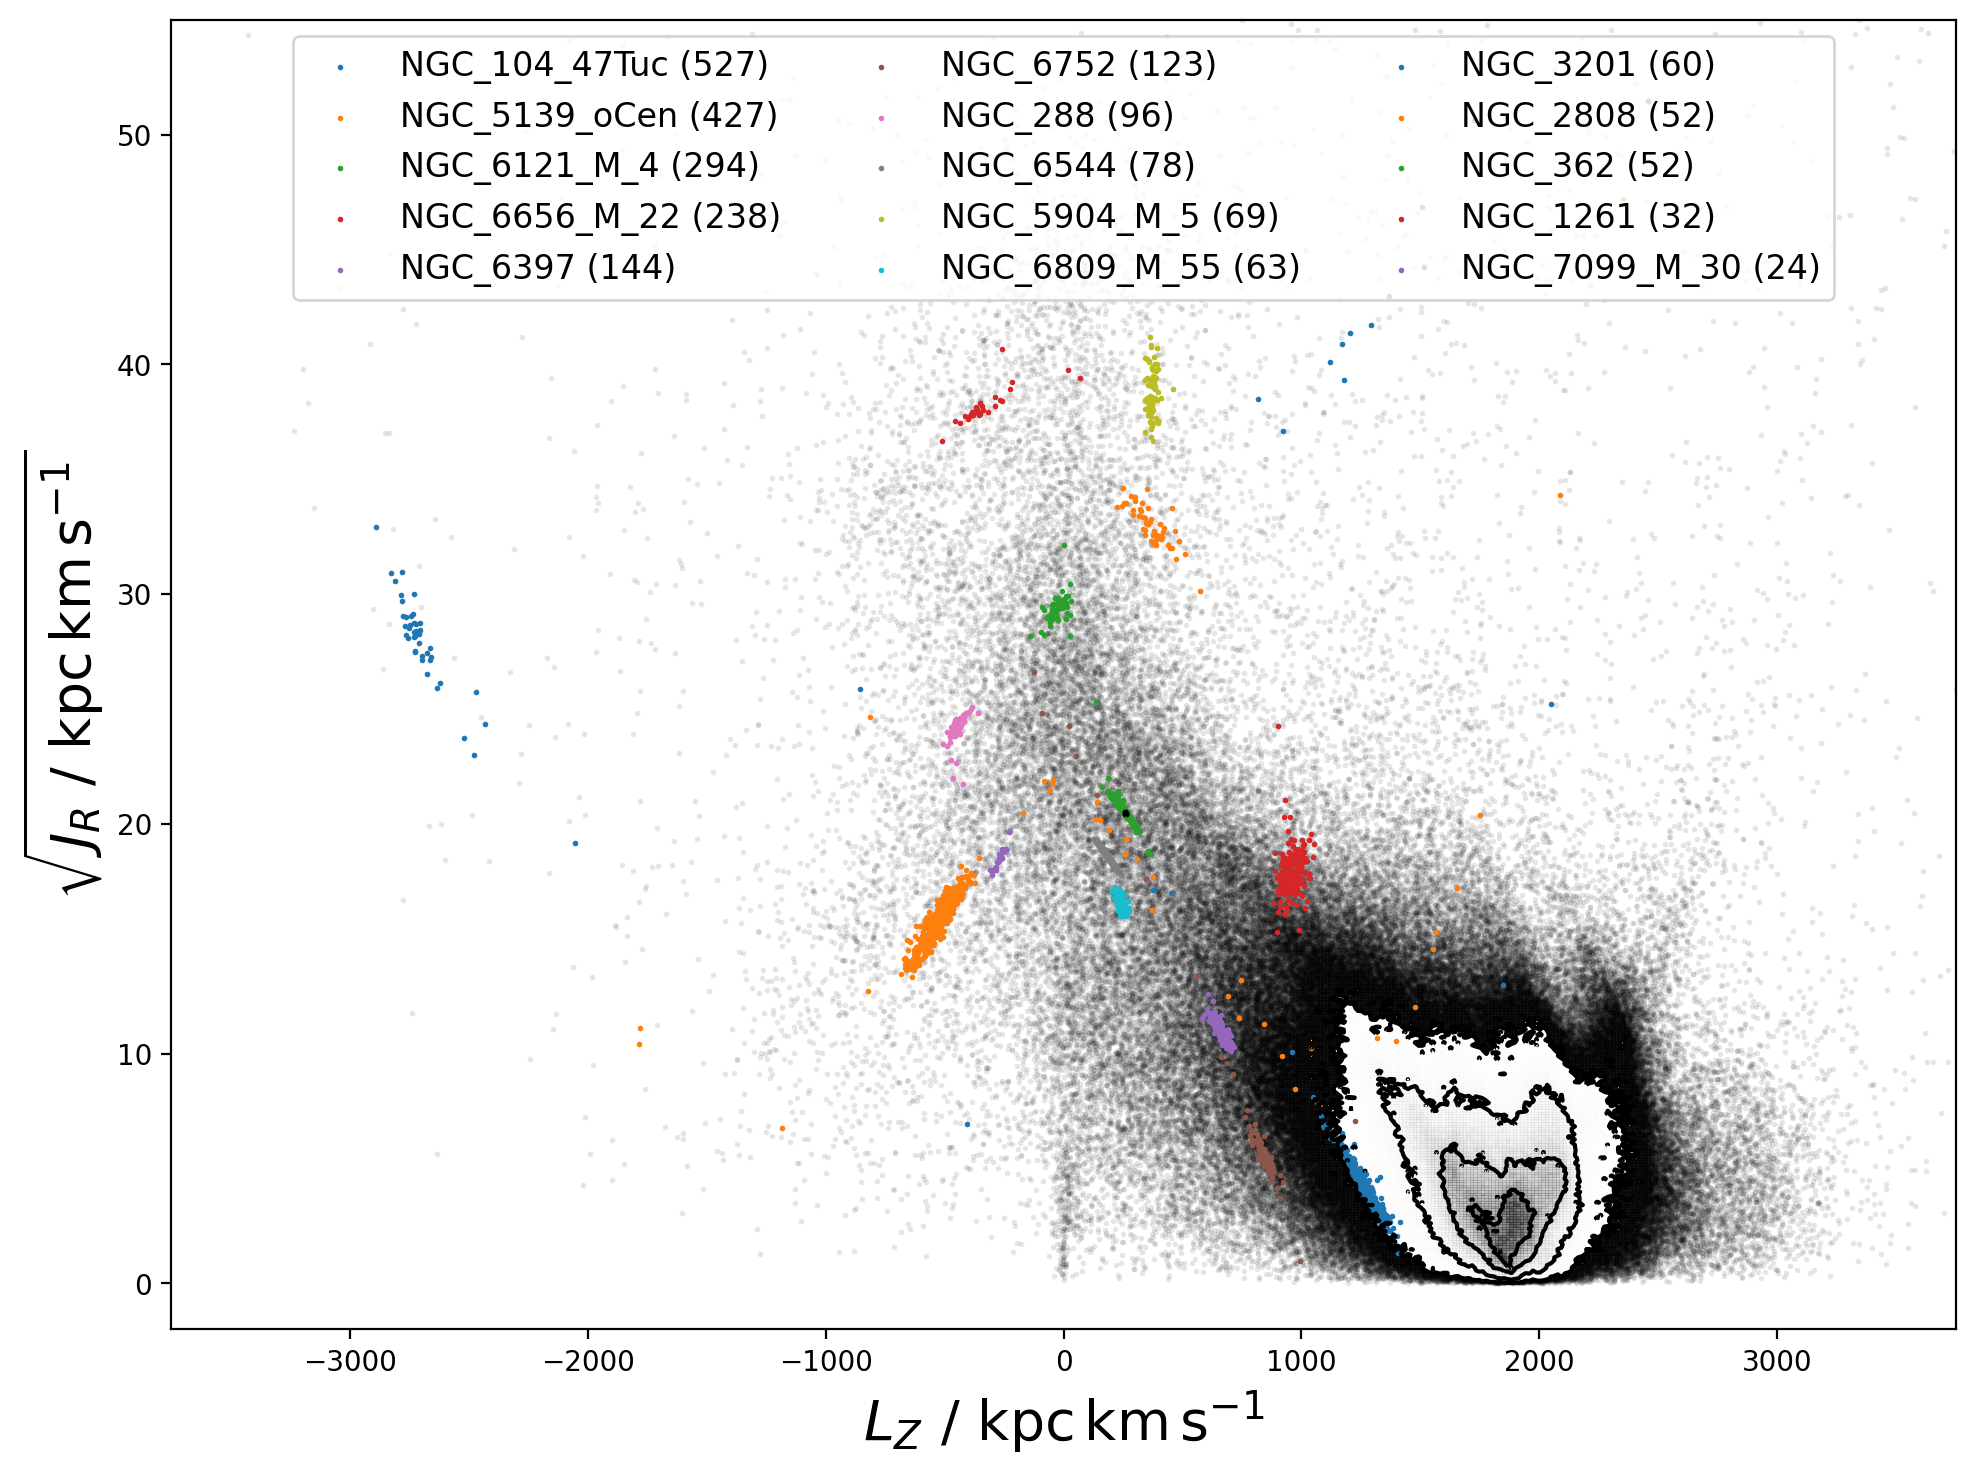
\includegraphics[width=0.975\columnwidth]{figures/galah_dr4_lz_jr_with_gcs.png}
\caption{
\textbf{Overview of the dynamical content of GALAH DR4 (black) as well as selected globular clusters (colored) in action space of angular momentum $L_Z$ versus radial action $J_R$.} Cluster members were selected as those with more than 70 percent membership probability according to \citet{Vasiliev2021}.
}
\label{fig:galah_dr4_lz_jr_with_gcs}
\end{figure}
\end{landscape}

\subsubsection{Ages}

\subsubsection{Crossmatches to \Gaia DR3, 2MASS and WISE}

\subsubsection{3D NLTE lithium abundances}

\section{CAVEATS AND FUTURE IMPROVEMENTS} \label{sec:caveats}

In this section, we attempt a detailed discussion of caveats along different steps of our analysis, while also giving suggestions for future improvements - both for GALAH and other surveys. We first discuss caveats of the spectrum reduction (Section~\ref{sec:caveats_reduction}), before extensively discussing the spectrum synthesis (Section~\ref{sec:caveats_synthesis}) and spectrum interpolation (Section~\ref{sec:caveats_interpolation}). We discuss possible problems arising from the use of photometric information (Section~\ref{sec:caveats_photospec}), in particular for stars that could be binaries (Section~\ref{sec:caveats_binaries}). While we have attempted to already flag possible caveats, we also lay out problematic flags in (Section~\ref{sec:caveats_flags}). We summarise the most important caveats in Section~\ref{sec:caveats_summary}.

\subsection{Spectrum reduction}  \label{sec:caveats_reduction}

Although a significant amount of work was spent on improving the spectrum reduction, we want to lay out a few areas that could still suffer from imperfection.

\subsubsection{Unreliable wavelength solutions}

For each CCD, the reduction pipeline estimates the most suitable wavelength solution, linking pixels with actual wavelengths based on the ThXe arc lines. In GALAH DR3 \citep{Buder2021} we identified several issues for spectra where not enough ThXe lines could be used to constrain the wavelength solution. Improvements have been made for the new reduction version to improve the number of useful ThXe lines. This has helped us to decrease the amount of problematic wavelength solutions towards the end of CCD3, with the only used absorption lines of Li and Eu, from an initially bad wavelength solution for 7.9\% of the spectra.

\subsubsection{Holistic spectrum extraction}

Although much work has been spent on improving telluric and sky lines in the reduction step, most reduction steps are currently run sequentially rather than in parallel. Using the information of stellar spectra when modelling the wavelength solution would certainly help to overcome the limited information in ThXe calibration spectra in the absence of laser combs \citep{Kos2018b}. Multiple steps towards this direction have been taken \citep{Saydjari2023} and should be rolled out in future spectrum analysis. This would especially help to mitigate imperfect telluric and sky line removal while simultaneously improving the wavelength solution - among many other effects.

\subsection{Imperfect spectrum synthesis} \label{sec:caveats_synthesis}

\subsubsection{Spectrum synthesis}

The GALAH survey's success is relying heavily on the ability to accurately model stellar spectra to infer accurate stellar properties. The survey has seen significant improvements in moving from the approximation of 1-dimensional (1D) atmospheres with local thermodynamic equilibrium (LTE) towards 1D NLTE, that is, statistical - or non-local - thermodynamic equilibrium \citep{Amarsi2020}. This includes the use of 1D NLTE synthesis for H \citep{Amarsi2018}, Li \citep{Lind2009, Wang2020}, C \citep{Amarsi2019}, N \citep{Amarsi2020b}, O \citep{Amarsi2018b}, Na \citep{Lind2011}, Mg \citep{Osorio2015}, Al \citep{Nordlander2017}, Si \citep{Amarsi2017}, K \citep{Reggiani2019}, Ca \citep{Osorio2019}, Mn \citep{Bergemann2019b}, Fe \citep{Amarsi2018, Amarsi2022}, and Ba \citep{Gallagher2020} for the {\sc marcs} model atmosphere grid. The work by \citet{Wang2024} also enables us to present measurements of Li in 3D NLTE as part of this release.

All of these advances are however contrasted by the lack of a proper way of modelling molecular features appropriately. This could explain the significant mismatch of oxygen abundances between optical and infrared \citep[compare e.g.][]{Bensby2014, SDSSDR17}. It can however also lead to mismatches in the GALAH wavelength range, where atomic features, such as \ion{C}{I}, can be modelled in 1D NLTE, whereas much often stronger molecular features of C2 and CN have to be modelled in 1D LTE.

For our synthesis, we have employed version 580 of the IDL-based code Spectroscopy Made Easy \citep{Valenti1996, Piskunov2017}. As part of the continuing improvement of this code, several bugs have been identified and fixed since. We also note that a python-based version of SME, \textsc{pySME} \citep{Wehrhahn2021}, has become available. In addition, the spectrum synthesis package \textsc{KORG} \citep{Wheeler2023, Wheeler2024} is currently undergoing the implementation of 1D NLTE synthesis, which is vital for its application on many of the NLTE-sensitive lines, such as O and K, in the GALAH wavelength range.

\subsubsection{Mismatch of atmosphere and spectrum chemistry}

For several of our synthetic spectra, the chosen chemical composition differs significantly from the scaled-Solar pattern of the \marcs model atmospheres. We note that APOGEE DR17 \citep{SDSSDR17} have computed \marcs atmospheres that matched their chemical compositions.

\subsection{Spectrum interpolation with neural networks} \label{sec:caveats_interpolation}

\subsubsection{Training set selection should be done after zeropoint corrections}

Before the neural networks are computed, it should actually be tested, what the abundance zeropoints are. In the case of several elements, like Na, Al, Eu, they were significant on the order of 0.2-0.3dex. In that case, stars with high abundances of 0.7-0.8 dex are not be sufficiently covered, although expected (e.g. in old stars and especially globular clusters). -> rerun neural networks for these cases?

\subsubsection{Masking of spectra}

Because the correlation of spectral features and stellar parameters and abundances is often complex, degeneracies can arise when two stellar properties influence similar pixels of a spectrum (e.g. C and N for CN, or \Teff and \feh for cool dwarfs) or two stellar properties tend to act in lockstep in actual stars (e.g. Mg, Si, and Ti as alpha-process elements). In GALAH DR2 \citep{Buder2018}, we have tried to overcome these issues by specifically masking the coefficients of spectrum interpolation, that is, effectively restricting the interpolation to only change smaller parts of the spectrum for a given stellar property.

In GALAH DR4, we have relaxed this restriction again, since we have trained on random abundance combinations in the hope of being able to break correlation degeneracies. We note, however, that too little information in spectra can again cause by-chance correlations (e.g. if neutron-capture lines are always very weak and the training set is not sufficiently large). We believe that this is the cause of the decrease in precision for Eu measurements from GALAH DR3 to GALAH DR4. The Eu line was mainly measured only from the weak Eu6645 line, whereas the neural networks are not restricted to this region.

\subsubsection{Flexibility of neural networks in general}

The choice of using a large number neural networks for restricted regions in the \TLF space was done based on the hope that they would require less flexibility from neural networks and thus a smaller network architecture. It has to be acknowledged that due to the limit of human power to properly train and test the neural networks, the chosen network architecture of a 2-layer perceptron with 300 neurons and a fixed learning rate is certainly imperfect at best. For this data release, we have decided to not rerun these steps, but make the current results available to the community. In the future, the restriction to one or only a few network models is recommended. The latter could cover regions of cool dwarfs, MSTO stars, hot stars, and giants stars with individual models - and possible explore the split in metal-poor and solar-like regimes. This would also decrease overhead, in particular for training and loading diferent models, and would also decrease possible noding effects between different models.

\subsubsection{Flexibility of neural networks for extreme abundances}

While this approach has proved to be powerful for all elements across their abundance ranges, we have noticed sinusoidal shapes for weak Li lines \citep[see also][]{Wang2020}. This is likely caused by the large dynamical range that has to be covered by the neural network of $0 < \mathrm{A(Li)} < 4$. For Li, the more sophisticated work of fitting Gaussian lines to multiple components in the wavelength range around $6708\,\text{\AA}$ is actually delivering appropriate measurements of EW(Li), which are then used to infer 3D-NLTE based A(Li) abundances. This inference is preferable to our 1D-NLTE based neural network estimates, as it is independent of the network flexibility and superior to our less accurate spectrum synthesis in 1D.

While several studies have identified that the abundances of stars in the Galactic disk are often very similar \citep[e.g.][]{Ness2019b}, the Galactic halo offers a more divers picture. An example is 2MASS J22353100-6658174 (140707003601047), a turn-off star with extremely high s-process abundances and actually visible lines of La and Nd in addition to the usually visible Y and Ba. In this case, the fits to the La and Nd lines are significantly weaker than the observations. GALAH DR3 actually produced reasonable fits to this star with high abundances in [Y/Fe]=1.2, [Ba/Fe]=1.5, [La/Fe]=1.5, [Ce/Fe]=1.1, [Nd/Fe]=1.9, and [Sm/Fe]=1.2. A neural network that is not trained on such high abundances is likely to improperly extrapolate stellar spectra.

While we have tried to stars with diverse abundance, such as carbon-enhanced metal-poor stars, the significant effect of their molecular features onto the whole stellar spectrum is not to be underestimated and can in-itself pose a problem to the flexibility of neural networks.

\subsubsection{Over- and underdensities at neural network edges}

While the use of one neural network to interpolate the high-dimensional spectrum space is preferable, in practise different science cases may drive the decision to use several networks.

If the science case is to reach maximum precision, one neural network that is trained on the typical spectrum could be used at the expense of properly modelling peculiar spectra.

If the science case is to reach maximum accuracy, only the regions with reliable line data and spectrum synthesis might be preferable.

If the science case is to find peculiar stars, a larger coverage is needed to avoid the inaccurate extrapolation of stars with extreme abundances.

In practice, large collaborations likely unite all of these goals, and a compromise has to be struck between the different approaches.

For future analyses, a possible solution could therefore be to follow a 2-step approach of first running one generic neural network for all spectra and then use optimised neural networks - or full spectrum synthesis - on smaller target samples of specific science cases.

\subsection{Mismatch of spectroscopic and photometric information} \label{sec:caveats_photospec}

\subsubsection{Incorrect masses driving incorrect stellar parameters}

We estimate masses and ages through isochrone matching, whose stellar parameters (validated against photometric estimates) is known for not being fully consistent with spectroscopic values.
We believe this leads to significant mismatches especially for stars close to the red clump. In this region, a small change in spectroscopic and photometric information can imply a significant change in inferred mass (e.g. from primary to secondary red clump, with the latter being 2 or more solar masses and thus significantly more than the usual $\sim$ 1 solar mass). This issue has only become noticeable after the production runs and we have therefore decided to not rerun this particular region of the parameter space for this data release. We have extensively tested the possible reasons and identified the mismatch of isochrones and actual stellar spectroscopic parameters as the cause. We have not been able to fully resolve this issue by either including an prior based on the initial mass function to weigh against massive stars \citep[see e.g.][]{Sharma2018} into the posterior mass estimates or artificially increasing the spectroscopic uncertainties when calculating the likelihood-weighted masses. More work needs to be done to mitigate the current inconsistencies of theoretical isochrones and spectroscopic estimates.

A solution for this particular region of the parameter space could be the use of chemical stellar evolution through the correlation of core and thus total mass and the ratio of [C/N] \citep{Masseron2015, Martig2016}, given that GALAH spectra also carry the information of both lines. This information could thus be used to better constrain high masses and counter-act the information from isochrone-inferred masses. For this data release, the [C/N] information could at least serve as an indicator of how trustworthy large giant star masses are.

\subsubsection{To use or not to use non-spectroscopic information?}

An implementation of non-spectroscopic information, as done in our \textit{allstar} module, has the advantage of overcome spectroscopic degeneracies (as proven for the limited information on \logg in the HERMES wavelength range) as well as improving accuracy and precision also for the lowest quality spectra (because \logg is no longer solely dependent on the spectrum information).

However, this approach is only useful if the non-spectroscopic information not biased (as it would be for astrometric and photometric information in the case of unresolved binarity). While the astrometric information for almost all GALAH targets is exquisite, this may not be the case for other surveys. The significant improvement from GALAH DR3 to GALAH DR4 has most definitely benefited from the improved astrometric infromation of \textit{Gaia} EDR3 \citep{GaiaEDR3, Lindegren2021a} and \textit{Gaia} DR3 \citep{GaiaDR3} with respect to \textit{Gaia} DR2 \citep{Brown2018, Lindegren2018}. Further improvement could be expected when also taking \textit{Gaia}'s photometric information into account, in addition to our use of 2MASS photometry.

\subsection{Binaries} \label{sec:caveats_binaries}

Although not part of this release, we have created an analysis module for spectroscopic binaries. The module will be presented in a separate work (Lach et al., in preparation) with a catalogue becoming a value-added-catalogue of this release. The module is motivated by the extensive study of GALAH binary star spectra by \citet{Traven2020} and our ability to model the full spectrum via neural networks. We show a first analysis result of the module in Fig.~\ref{fig:examples_flag_sp_3}, we the module was applied to a spectroscopic binary type 2 and is resulting in a significantly better fit than the single star analysis.

\begin{figure}[ht]
 \centering
 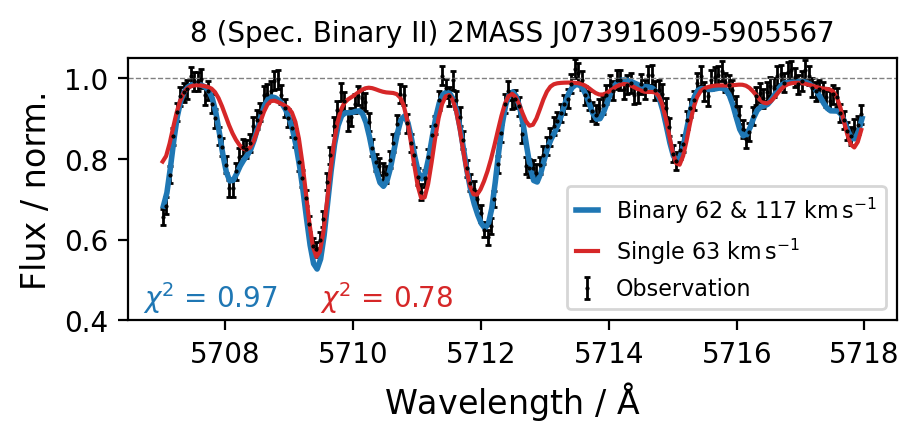
\includegraphics[width=\textwidth]{figures/examples_flag_sp_3.png}
 \caption{\textbf{Example spectrum for a double-lined spectroscopic binary star (SBII) that is better fit with our binary fitting algorithm.}} \label{fig:examples_flag_sp_3}
\end{figure}

\subsection{Reliability of flags} \label{sec:caveats_flags}

We have tried to develop a quality assurance pipeline that automatically flags results and stars that may not be adequately analysed with our assumptions.

\subsubsection{Bug in \texttt{flag\_fe\_h}}

The quality flag for iron abundance, \texttt{flag\_fe\_h}, was computed similar to the elemental abundances, that is by comparing the best-fit spectrum with a spectrum with the lowest grid value. In the case of \feh, however, this is a good approach. It can lead to a comparison of a spectrum with -0.74 to one with -0.75, which can easily be too similar within the signal-to-noise range. This likely affected 34\% of stars and we therefore do not recommend the use of this flag at all. In the future, such a test should be performed with respect to an actually low (undetectable) amount of iron, such as $\mathrm{[Fe/H]} = -4$.

\subsubsection{Fitting machinery stuck in local minimum}

We have tried to automatically identify regions of the parameter space, where the \textsc{scipy.optimize.curve_fit} function has gotten stuck at a local minimum. In particular for cool giants and some red clump stars, we have been able to recover a pattern of abundances being stuck around their initial value. Because of the zero point corrections, these are shifted away from the usual initial guess of $0\,\mathrm{dex}$ depending on the element (see Table~\ref{}

\subsubsection{Binary or fast rotating star?}

With the increasing amount of turn-off stars as part of ongoing GALAH observations, we have tried to implement a more sensitive approach to identify binaries in this region. This may, however, mean that we have also introduced more false-positive detections of stars that are only fast rotating with higher \vsini, rather than being a binary system. We therefore suggest to carefully consider using or neglecting the accompanying flag in GALAH DR4 (see Table~\ref{tab:flag_sp}).

\subsection{Summary of caveats} \label{sec:caveats_summary}

In summary, the most important caveats are:
\begin{itemize}
    \item Noding in \TLF around edges between neural networks: Our tests when switching between neural networks indicates that this effect for \TLF should stay within the precision uncertainties. A more difficult effect might be that some elements might be fit as part of one neural network based on the detectability tests that were performed at the grid centres of each neural network.
    \item Mismatches of photometry and spectroscopy: Both imperfect isochrone and spectrum models can drive a mismatch in the estimation of spectroscopic parameters. This is most notable around the secondary red clump region and also expected for highly extincted regions.
    \item Imperfect synthesis leading to trends in cool stars: The unreliable line data in cool stars is causing increasingly inaccurate models and inferred stellar properties towards the coolest stars.
    \item Lower precision for Eu due to missing masking of neural networks.
\end{itemize}

These caveats are the unfortunately negative effects of our attempt to increase the accuracy and precision of stellar parameters and elemental abundances while simultaneously pushing the number of stars for which we can report abundances.

%%%%%%%%%%%%%%%%%%%%%%%%%%%%%%%%%%%%%%%%%%%%%%%%%%%%%%%%%%%%%%%%%%%%%%%%%
\section{CONCLUSIONS}
\label{sec:conclusion}



%%%%%%%%%%%%%%%%%%%%%%%%%%%%%%%%%%%%%%%%%%%%%%%%%%%%%%%%%%%%%%%%%%%%%%%%%

%%%%%%%%%%%%%%%%%%%%%%%%%%%%%%%%%%%%%%%%%%%%%%%%%%
\section*{Acknowledgements}
%%%%%%%%%%%%%%%%%%%%%%%%%%%%%%%%%%%%%%%%%%%%%%%%%%

We acknowledge the traditional owners of the land on which the AAT and ANU stand, the Gamilaraay, the Ngunnawal and Ngambri people. We pay our respects to elders past, present, and emerging and are proud to continue their tradition of surveying the night sky in the Southern hemisphere.
This work was supported by the Australian Research Council Centre of Excellence for All Sky Astrophysics in 3 Dimensions (ASTRO 3D), through project number CE170100013.

\section*{Facilities}

\textbf{AAT with 2dF-HERMES at Siding Spring Observatory:}
AAT observations for this data release were performed under programs {2013B/13}, {2014A/25}, {2015A/3}, {2015A/19}, {2015B/1}, {2015B/19}, {2016A/22}, {2016B/10}, {2016B/12}, {2017A/14}, {2017A/18}, {2017B/16}, {2018A/18}, {2018B/15}, {2019A/1}, {2019A/15}, {2020B/14}, {2020B/23}, {2022B/02}, {2022B/05}, {2023A/04}, {2023A/08}, {2023A/09}, {2023B/04}, and {2023B/05}.

\textbf{AAO Data Central:} This paper includes data that has been provided by AAO Data Central  (datacentral.org.au) and makes use of services and code that have been provided by AAO Data Central.

\textbf{\Gaia: } This work has made use of data from the European Space Agency (ESA) mission \Gaia (\url{http://www.cosmos.esa.int/gaia}), processed by the \Gaia Data Processing and Analysis Consortium (DPAC, \url{http://www.cosmos.esa.int/web/gaia/dpac/consortium}). Funding for the DPAC has been provided by national institutions, in particular the institutions participating in the \Gaia Multilateral Agreement. 

\textbf{Other facilities:} This publication makes use of data products from the Two Micron All Sky Survey \citep{Skrutskie2006} and the CDS VizieR catalogue access tool \citep{Vizier2000}.

\section*{Software}

The research for this publication was coded in \textsc{python} (version 3.7.4) and included its packages
\textsc{astropy} \citep[v. 3.2.2;][]{Robitaille2013,PriceWhelan2018},
\textsc{astroquery} \citep[v. 0.4;][]{Ginsburg2019},
\textsc{corner} \citep[v. 2.0.1;][]{corner},
\textsc{galpy} \citep[version 1.6.0;][]{Bovy2015},
\textsc{IPython} \citep[v. 7.8.0;][]{ipython},
\textsc{matplotlib} \citep[v. 3.1.3;][]{matplotlib},
\textsc{NumPy} \citep[v. 1.17.2;][]{numpy},
\textsc{scipy} \citep[version 1.3.1;][]{scipy},
\textsc{sklearn} \citep[v. 0.21.3;][]{scikit-learn},
We further made use of \textsc{topcat} \citep[version 4.7;][]{Taylor2005};


\bibliography{bib}

\appendix

\section{Initial parameters}

\begin{figure*}[ht]
 \centering
 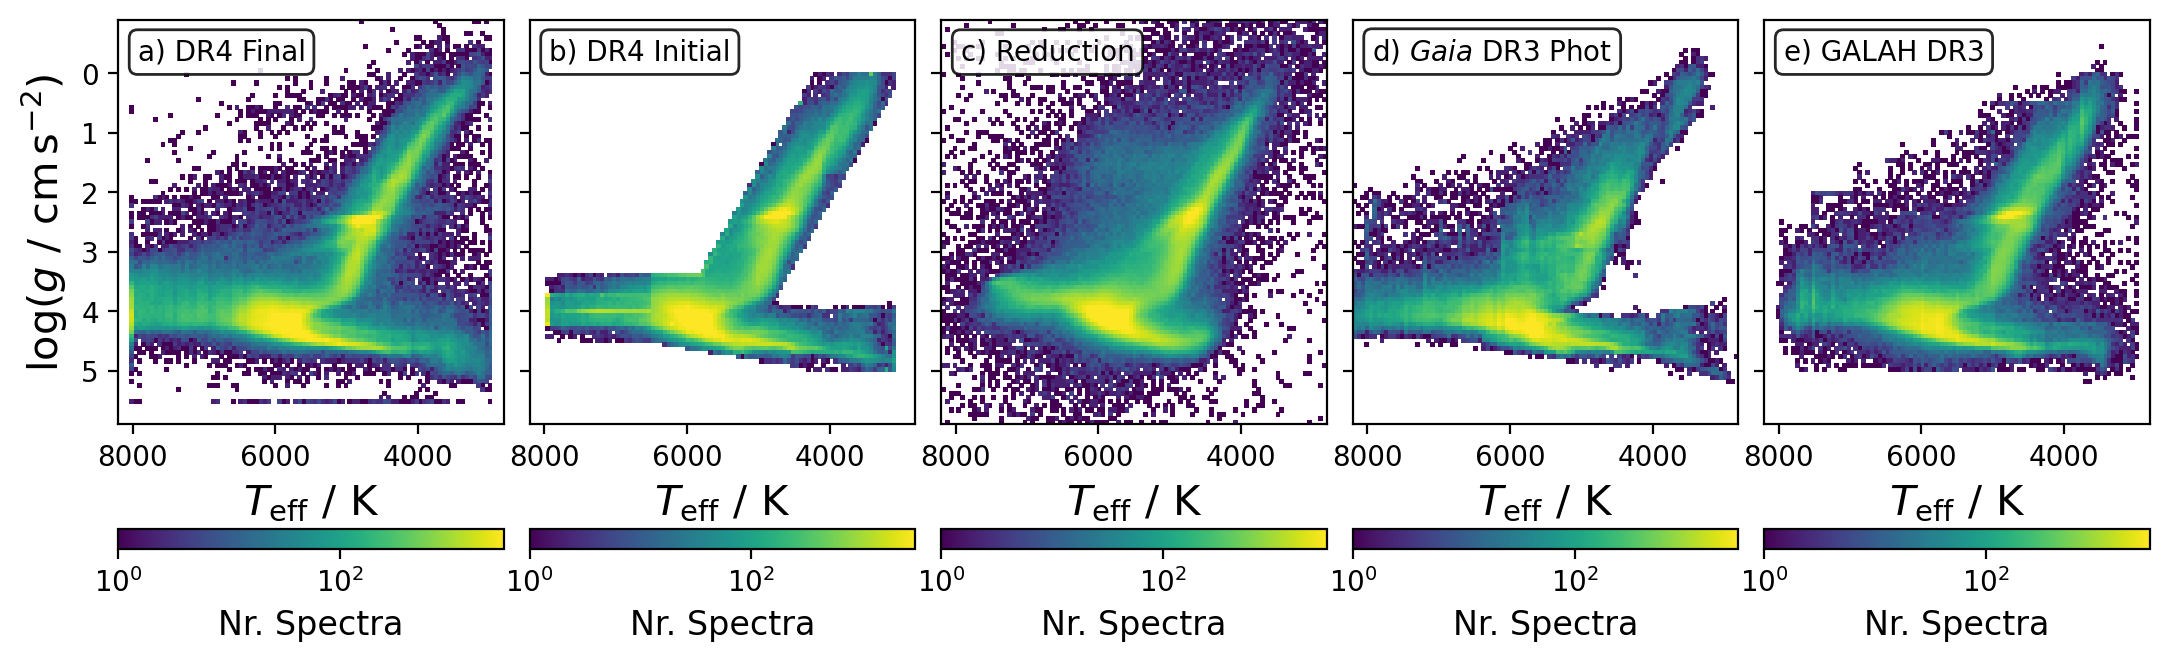
\includegraphics[width=\textwidth]{figures/initial_teff_logg.png}
 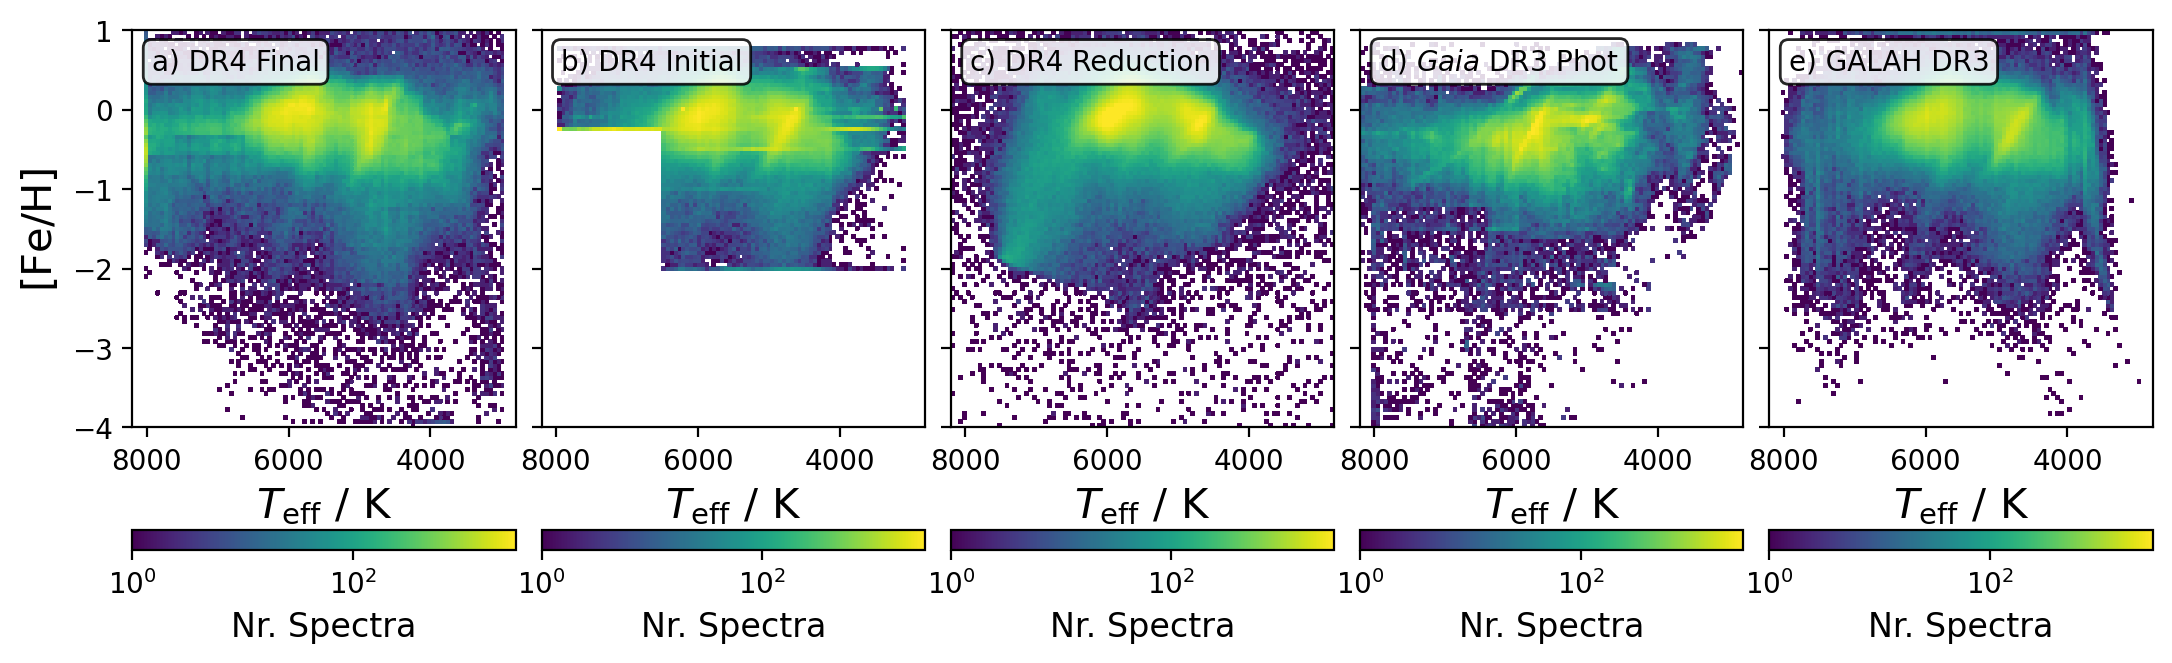
\includegraphics[width=\textwidth]{figures/initial_teff_fe_h.png}
 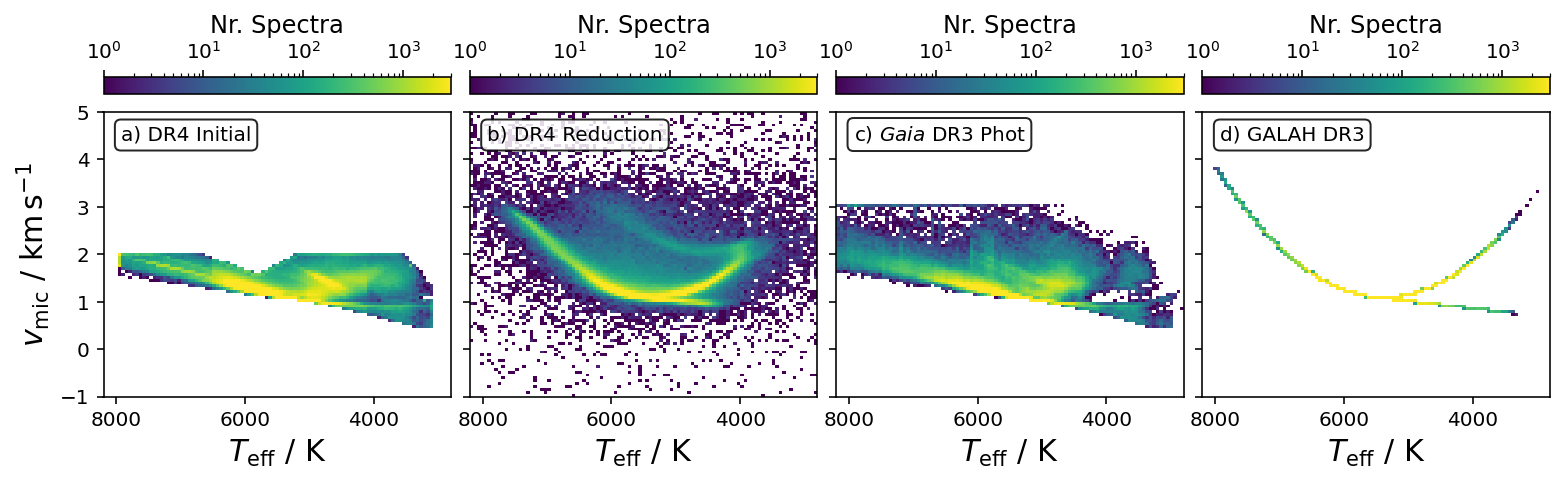
\includegraphics[width=\textwidth]{figures/initial_teff_vmic.png}
 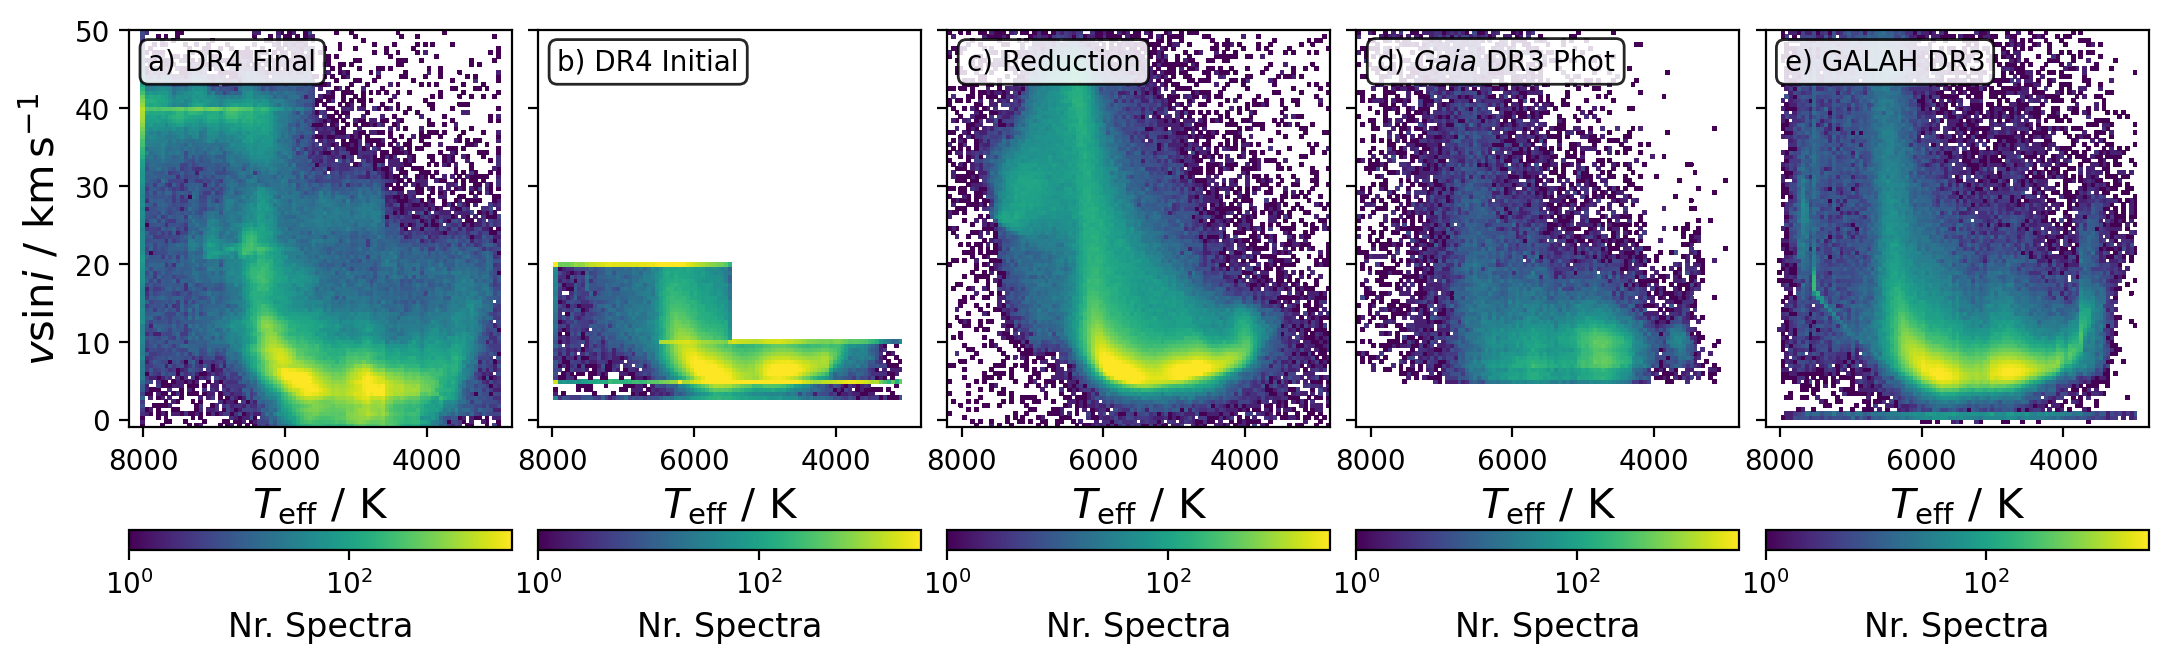
\includegraphics[width=\textwidth]{figures/initial_teff_vsini.png} \caption{\textbf{Comparison of final GALAH DR4 stellar parameters (first column) against the initial parameters used in the \textit{allsta} analysis (second column), estimates from the GALAH DR4 reduction pipeline (third column), \Gaia DR3 (fourth column with \vmic based on the adjusted formula from \citet{DutraFerreira2016}), and GALAH DR3 (fifth column).}} \label{fig:initial_parameters}
\end{figure*}

\section{Example Fit Comparison}

\begin{figure*}[ht]
 \centering
 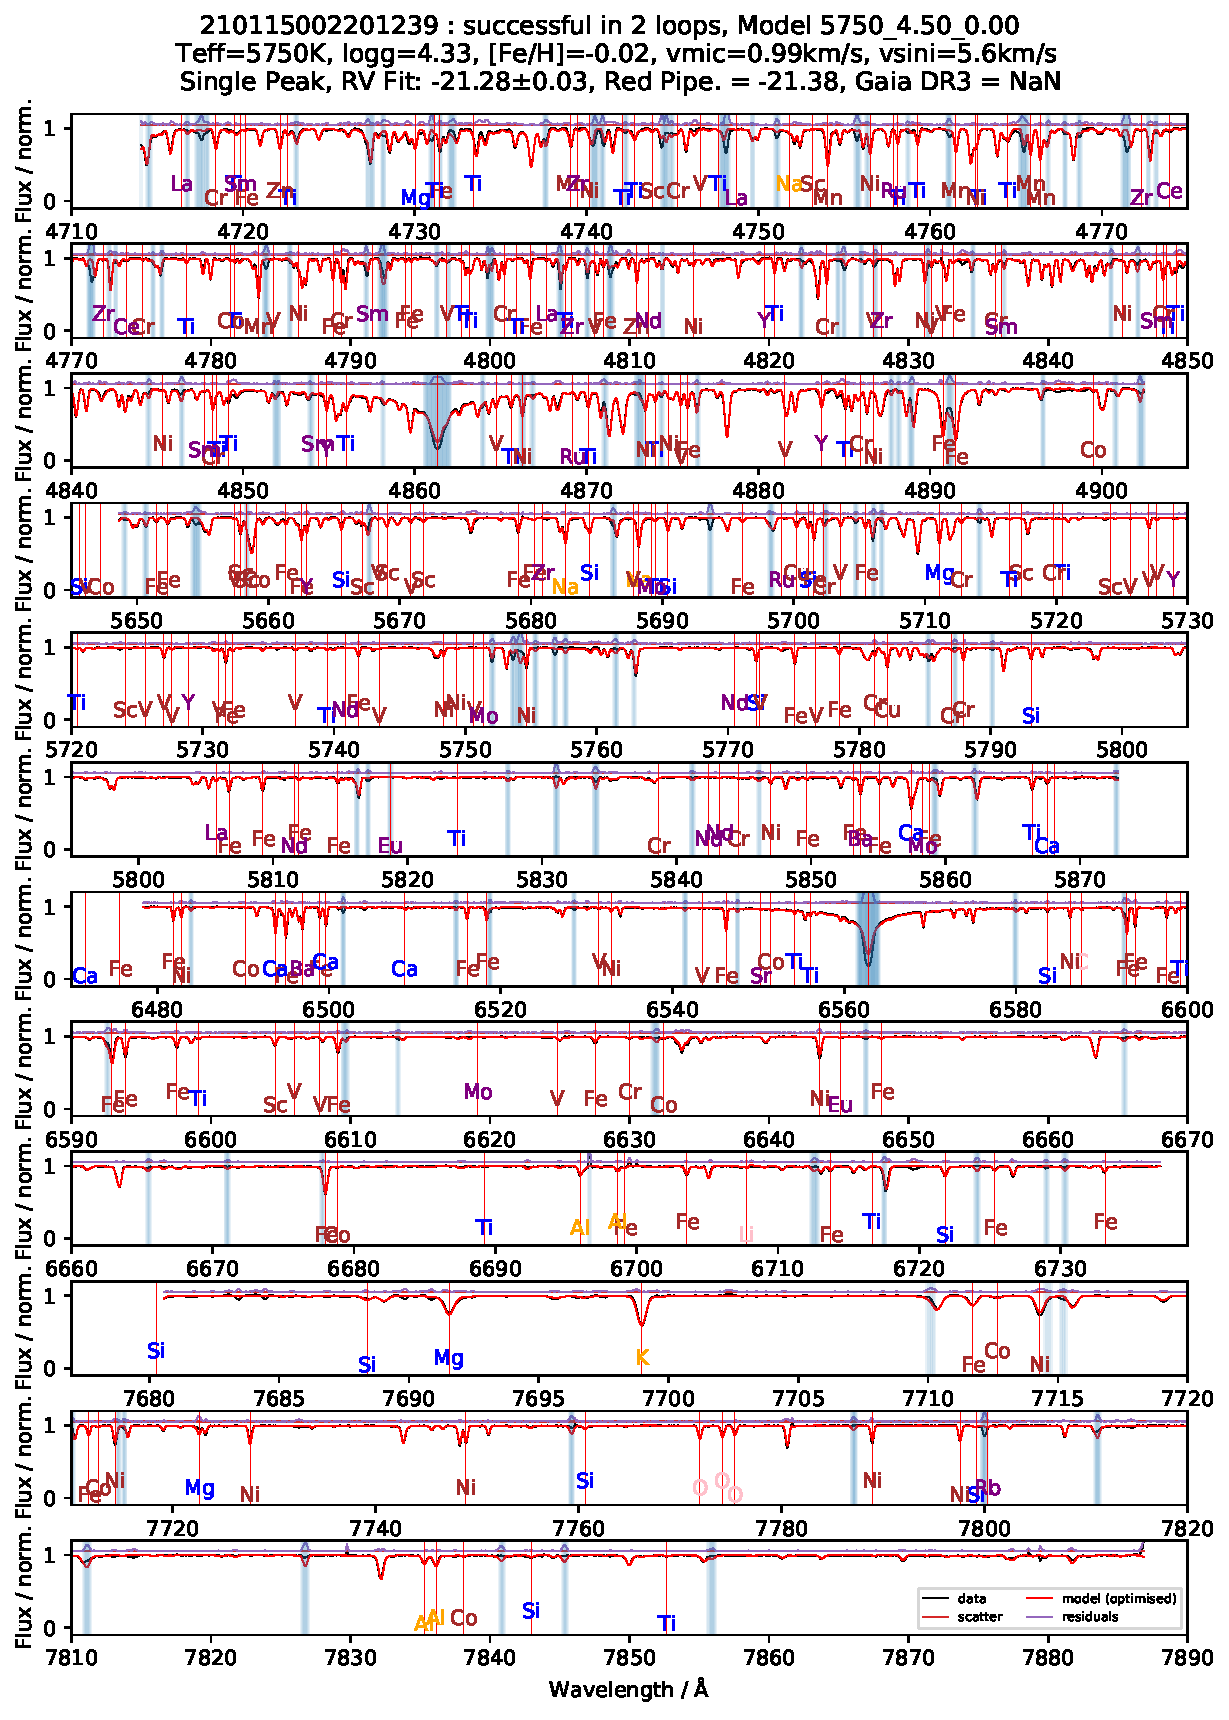
\includegraphics[width=0.9\textwidth]{figures/210115002201239_single_fit_comparison.pdf} \caption{\textbf{Example output of the \textit{allspec} fitting routine for Vesta / 210115002201239.}} \label{fig:210115002201239_single_fit_comparison}
\end{figure*}

\end{document}
